\documentclass[journal]{IEEEtran}

\usepackage{amsmath,amssymb}
\usepackage{graphicx}
\usepackage{booktabs}
\usepackage{multirow}
\usepackage{array}
\usepackage{cite}
\usepackage{url}
\usepackage{hyperref}
\usepackage{xcolor}
\usepackage{algorithm}
\usepackage{algpseudocode}
\usepackage{float}
\usepackage{pifont}

\title{Quantitative Evaluation of Explainable AI Methods for Gallbladder Diseases through Ultrasound Images}

\author{
\parbox{0.9\linewidth}{\centering
Sayed Ifti Ahmed\textsuperscript{*}\quad Mst.~Khadiza Akter Sammi\textsuperscript{*}\\[4pt]
\normalsize Department of Computer Science and Engineering, Daffodil International University (DIU), Dhaka, Bangladesh\\[2pt]
ifti241-15-227@diu.edu.bd \quad akter241-15-704@diu.edu.bd\\[2pt]
\textsuperscript{*}Equal contribution.
}
}

\begin{document}

% Figures/tables were drifting far from their in-text references (e.g. Fig. 1,
% cited on page 3, was not placed until page 19) under IEEEtran's default
% float-eligibility thresholds combined with [tb]-style deferred placement.
% These must be set after \begin{document} -- IEEEtran resets them internally
% at class-load time, so setting them before \begin{document} has no effect.
\renewcommand{\topfraction}{0.95}
\renewcommand{\bottomfraction}{0.95}
\renewcommand{\textfraction}{0.05}
\renewcommand{\floatpagefraction}{0.75}
\setcounter{topnumber}{6}
\setcounter{bottomnumber}{6}
\setcounter{totalnumber}{10}

\maketitle
\thispagestyle{empty}
\pagestyle{plain}

\begin{abstract}
Deep-learning studies on gallbladder ultrasound usually give accuracy and a handful of heatmaps as proof of interpretability, and rarely test whether either one survives closer scrutiny. This paper does that scrutiny directly, on a ResNet-50 trained for nine-class gallbladder ultrasound classification on the public UIdataGB dataset, and the scrutiny itself is what changes the headline number. An initial split, de-duplicated only by single-orientation image hashing, gave 93.05\% accuracy; a closer audit found that split still let near-identical frames from the same imaging session, and rotation-augmented duplicates the dataset's own release pipeline introduces, cross the train/validation boundary. Correcting for both---clustering images at the session level and by an 8-orientation perceptual hash, then holding out a genuine test set touched only once---drops mean accuracy across four independently seeded models to 72.56\% $\pm$ 2.35\%. We report this corrected figure as the paper's real result, not the inflated one. The main XAI evaluation---five attribution techniques (Grad-CAM, Grad-CAM++, Saliency Maps, Eigen-CAM, and Score-CAM) compared for consistency across replicate models, faithfulness, stability, a parameter-randomization sanity test, a shortcut audit, and calibration---was run on the uncorrected, higher-accuracy split, and Grad-CAM++ and Score-CAM are the most reproducible across seeds there; on faithfulness all three CAM methods perform similarly, and no single method wins on every metric. Because the reproducibility replicates in that battery were trained on disjoint data subsets rather than identical data with only the seed varied, we separately reran the consistency check under a corrected same-data design on the leakage-fixed split, using Grad-CAM as a representative method, together with a null-control test---cosine similarity between untrained models and between synthetic random heatmaps---that the original metric had not been checked against. The corrected same-data consistency score clears both null floors by roughly 2.5$\times$ rather than sitting close to them, so the consistency finding survives this check, though it has not yet been re-verified for all five methods under the corrected design. Grad-CAM++'s output depends on the model's learned weights rather than the architecture alone, and while we find no strong sign the model relies on image-border artefacts specifically, a separate, targeted audit finds a real batch-correlated shortcut: a classifier trained only to identify which acquisition batch a Carcinoma image came from reaches 82.88\% accuracy (8.3$\times$ chance) even after correcting for cluster-level leakage, and a linear probe on the disease classifier's own features recovers batch identity at 74.75\% (4.5$\times$ chance), directly implicating the classifier this paper's explanations describe. The results show these attributions are measurably faithful to the classifier's behaviour; that is not the same as proof the classifier's decisions are clinically reliable, and the batch-shortcut finding above is a concrete reason for caution beyond the usual internal-validation caveats. This remains an internal-validation study: it does not establish multicentre generalizability, patient-level validation, or clinician-confirmed localization, and several methodological gaps identified during external review---including bootstrap intervals for the XAI metrics (now added for the consistency, faithfulness, and stability tables), a full re-run of the five-method battery on the corrected split, and validation of the session/batch inference used in the split correction---remain open and are reported honestly rather than elided.
\end{abstract}


\begin{IEEEkeywords}
Gallbladder ultrasound, explainable artificial intelligence,
data leakage, shortcut learning, grouped validation, Grad-CAM,
deep learning, internal validation.
\end{IEEEkeywords}

\section{Introduction}

Gallbladder diseases---cholelithiasis, cholecystitis, polyps, adenomyomatosis, carcinoma, GBC---affect hundreds of millions worldwide. GBC is especially deadly when caught late; five-year survival drops below 20\% \cite{ref1}, \cite{ref2}. Ultrasound is the go-to first-line scan for the gallbladder. Yet a systematic review and meta-analysis shows its sensitivity for acute cholecystitis sits at a mere 81\% (studies range from 50\% to 100\%) and specificity at 83\% (33\% to 100\%). That spread mirrors real-world operator and protocol variation \cite{ref3}. Such inconsistency pushes us toward computer-aided classification, a decision-support tool, while also highlighting the promise and the caution that accompany AI in medicine \cite{ref4}, \cite{ref5}, \cite{ref6}. CNNs now match or outshine earlier gallbladder-ultrasound classifiers \cite{ref7}, but clinical uptake stalls at opacity. A CNN is a black-box: it spits out a verdict without showing why. Radiologists need visual proof that the model is looking at real anatomy---wall irregularity, acoustic shadowing, lumen echogenicity---rather than noise or artefacts \cite{ref9}, \cite{ref10}.

XAI techniques---Grad-CAM \cite{ref11}, Grad-CAM++ \cite{ref12}, gradient saliency maps---offer class-discriminative heatmaps. A heatmap that appears anatomically plausible is not proof of reliability. Ghassemi et~al. \cite{ref9} and Rudin \cite{ref8} note that most clinical XAI studies stop at visual inspection, never checking if the explanation actually points to the right area, survives small changes, reflects the true driver of the prediction, or repeats across separate training runs. Sanity-check studies \cite{ref13} and interpretability benchmarks \cite{ref14} reveal that some popular saliency methods fail these tests yet still look convincing. A convincing heatmap alone is insufficient; we must quantify reliability.

Earlier gallbladder-ultrasound studies have employed XAI, and at least one provided clinician-grounded, quantitative localization evidence \cite{ref19}. Yet a structured, non-systematic literature review (Section~\ref{sec:related-work}) found no peer-reviewed work that pulls together a multi-method post-hoc attribution comparison with quantitative metrics for cross-training consistency, perturbation-based faithfulness, explanation stability. And sensitivity to learned parameters---all within one framework. When several XAI methods appear together in this field, they tend to be compared qualitatively, not measured along these reliability dimensions. This paper asks: how much does the choice of XAI method influence a nine-class gallbladder-ultrasound classifier. And are the explanations reproducible or just artifacts of a single training run? The goal is not to introduce XAI to gallbladder ultrasound---previous work has done that---but to quantitatively test whether common post-hoc visual explanations are reliable. We tackle this with a multi-method, quantitatively evaluated XAI analysis, confined to a single public dataset and evaluated at the image level. The dataset's original publication says the images came from three to four hospitals in Baghdad, Iraq. But the public release strips away hospital, patient, or scanner IDs, so we cannot recover or stratify site provenance (Section~\ref{sec:methods}.1). We make the scope clear: this is an internal-validation study on data with unknown provenance, not a claim of external multicentre generalizability or clinical deployment. Those larger questions will guide the validation programme we start here (Section~\ref{sec:future-research}).

Our work has five aims. First, we train and test a ResNet-50 to perform nine-class gallbladder-ultrasound classification. Second, we apply five XAI methods---Grad-CAM, Grad-CAM++, Saliency Maps, Eigen-CAM, Score-CAM---to the same trained model. So we can compare them head-to-head instead of looking at one in isolation. Third, we calculate a cosine-based consistency score to see if each method's explanation stays the same across independently trained model replicas. Fourth, we test faithfulness by deletion/insertion against a random control. Fifth, we assess stability under clinically invariant image transforms and check if the explanations hinge on learned weights rather than just the architecture, using a parameter-randomisation sanity check. Alongside, we calibrate the classifier's predicted probabilities with temperature scaling, so the XAI outputs can be paired with trustworthy confidence values.

This paper offers six contributions. First, a two-stage leakage audit of the UIdataGB release itself: an initial split de-duplicated only by single-orientation perceptual hashing looked clean but still let near-identical frames from the same imaging session, and rotation-augmented duplicates the dataset's own release pipeline introduces, cross the train/validation boundary; correcting both drops mean accuracy from an inflated 93.05\% to an honestly-measured 72.56\%~$\pm$~2.35\% across four independently seeded models on a genuine, cluster-aware held-out test set. We treat this correction, and the willingness to report the lower number, as a contribution in its own right, not a footnote. Second, a quantitative XAI benchmark that runs five methods---Grad-CAM, Grad-CAM++, Saliency Maps, Eigen-CAM, Score-CAM---on a ResNet-50 gallbladder-ultrasound model, covering more methods and classes than any previous study (see Table~\ref{tbl:9}). Third, a quantitative XAI-reliability suite: cosine-based cross-replicate consistency $O^c$, faithfulness tests, stability checks, a model-randomisation sanity check, calibration, and a shortcut audit, together with a null-control test of the consistency metric itself against untrained-model and synthetic-heatmap floors, which the metric had not previously been checked against. This moves us past ``heatmaps that look right'' to explanations that are actually measured to be reliable. Fourth, a failure-case analysis grounded in clinician-affirmed evidence that looks at specific high-confidence misclassifications instead of just overall accuracy. Fifth, an honest validation roadmap that spells out what remains to be proven, especially clinician-annotated localization and a full re-run of the five-method XAI battery on the corrected split (Section~\ref{sec:future-research}). Sixth, open reproducibility. All XAI code ships with this submission, and trained checkpoints and generated figures will go to a permanent public archive once the paper is accepted.

Here is how the rest of the paper unfolds. Section~2 covers background and related work, and Section~3 lays out the materials and methodology. Section~4 presents classification and XAI results. Section~5 discusses what they mean, their clinical relevance, reliability, how they relate to prior work, limitations, and future directions. Section~6 wraps things up.

\section{Background and Related Work}
\label{sec:related-work}

The literature reviewed below was identified through a structured, non-systematic search of gallbladder-ultrasound AI and medical-XAI publications (2016--2026). It followed the spirit of search-transparency practice recommended for systematic reviews \cite{ref15}. This is a narrative review, not a formal systematic one.

Conventional CAD systems for gallbladder imaging relied on hand-crafted texture features and classical classifiers \cite{ref16}. Deep learning has since substantially improved performance on this task. Turki et~al. \cite{ref17} released the multi-class UIdataGB gallbladder ultrasound dataset used in this paper. It spans nine disease classes drawn in part from ultrasound video sequences. Their dataset-release publication reports that the underlying images were collected across three to four hospitals in Baghdad, Iraq, over four years, on four different ultrasound scanner models. The public release itself, still, carries no hospital, patient, or scanner identifier. So this multi-site provenance cannot be recovered or stratified on from the released files (Section~\ref{sec:methods}.1).

Using the same 10,692-image, 1,782-patient collection, Obaid et~al. \cite{ref18} reported 98.35\% accuracy with a MobileNet classifier across all nine classes. They evaluated it with a single CAM variant, reporting the results qualitatively rather than through a quantitative, multi-method XAI comparison. Two more recent studies on this dataset use more than one XAI method. Nabil et~al.'s MSFE-GallNet-X \cite{ref57} applies both Grad-CAM and LIME. Kumar et~al. \cite{ref58}, on a related cholelithiasis-focused ultrasound task, combine Grad-CAM and LIME into a hybrid explanation. Both report their explanations qualitatively, as illustrative heatmaps, rather than with the quantitative cross-method, cross-replicate, or faithfulness metrics applied here. They show that multiple XAI methods have been used together for gallbladder ultrasound. This narrows, but does not close, the gap this paper addresses (see the gap statement below).

A parallel line of work has built classifiers on a separate, five-class gallbladder-ultrasound dataset (GBCU). Basu et~al. \cite{ref7} released GBCU alongside curriculum-learning ResNet classification, and RadFormer \cite{ref19} added global-local transformer attention for interpretable GBC detection on the same dataset. Gupta et~al. prospectively evaluated deep learning for GBC detection on ultrasound \cite{ref20}. They also studied a multiple-instance-learning approach across several explicitly identified centres \cite{ref21}. This kind of externally validated, site-stratified evaluation is something this paper's single, site-unlabelled dataset release cannot support. More recent 2024--2025 work has pushed accuracy further. Anatomy-aware architectures on GBCU appear in Hasan et~al.'s GBCHV \cite{ref22}. Video-based masked autoencoder detection shows up in Basu et~al.'s FocusMAE \cite{ref23}, building on an earlier weakly-supervised variant \cite{ref24}. Other work addresses gallbladder polyp classification specifically \cite{ref16}, \cite{ref25}, \cite{ref26}. With the partial exception of RadFormer's attention maps, none of these studies, on either dataset, compares multiple XAI methods quantitatively or tests reproducibility across independent training runs.

Deep convolutional networks are now the dominant approach across medical-imaging classification generally. And transfer learning from ImageNet-pretrained backbones such as ResNet \cite{ref27}, DenseNet \cite{ref28}, and EfficientNet \cite{ref29} is standard practice for small medical datasets \cite{ref30}. That performance gain carries a well-documented cost, though: such models are widely regarded as ``black boxes,'' and clinical adoption depends on being able to inspect, not merely trust, the reasoning behind a prediction \cite{ref8}. Surveys by Tjoa and Guan \cite{ref31}, van der Velden et~al. \cite{ref10}. And the edited volume of Samek et~al. \cite{ref32} converge on the same caution. Qualitative heatmap visualisation is the most common form of ``explanation'' reported in clinical deep learning. It is routinely treated as sufficient evidence of interpretability on its own, without further testing \cite{ref8}, \cite{ref9}.

Selvaraju et~al. \cite{ref11} proposed Grad-CAM. It weights a convolutional layer's feature maps by the gradient of the target class score. Chattopadhay et~al. \cite{ref12} introduced Grad-CAM++. They replaced globally average-pooled weights with pixel-wise weighted second-order derivatives, giving sharper localisation of small or multiple lesions. Vanilla gradient saliency \cite{ref33} takes the gradient of the class score directly with respect to input pixels. The result is noisier but at pixel resolution. Unlike the CAM family, it needs no target-layer choice. It still requires differentiable, white-box access to gradients, so it is architecture-agnostic, not model-agnostic in the stricter sense that applies to input/output-only methods below. Muhammad and Yeasin \cite{ref34} proposed the class-agnostic, gradient-free Eigen-CAM. It projects a layer's activations onto their dominant principal component. Wang et~al. \cite{ref35} proposed the gradient-free Score-CAM. It weights each activation channel by its measured effect on the model's own output when used as an input mask. This avoids gradient saturation but costs extra compute. Beyond these five, model-agnostic methods such as SHAP \cite{ref36} and LIME \cite{ref37} and gradient-based variants such as Integrated Gradients \cite{ref38} and LayerCAM \cite{ref39} broaden the attribution landscape. But they fall outside the scope of this paper. Section~\ref{sec:methods}.3 gives the full formulation of each of the five methods used here.

A growing body of work argues that visual plausibility alone is not enough for medical XAI. Adebayo et~al. \cite{ref13} found that several popular saliency methods do not respond to model or label randomisation. That sanity check should make any trustworthy method fail loudly. Hooker et~al. \cite{ref14} created the ROAR benchmark, which compares methods by feature-removal faithfulness. Ghassemi et~al. \cite{ref9} and Rudin \cite{ref8} make a related point: post-hoc explanation methods get over-trusted in healthcare without this kind of quantitative scrutiny. Geirhos et~al. \cite{ref40} gave shortcut learning its name and formal definition. Zech et~al. \cite{ref41} showed a real case of it in medical imaging, where a pneumonia classifier partly learned hospital-specific image artefacts instead of pathology. That is exactly the failure mode the shortcut audit in Section~\ref{sec:results}.4 is built to catch. Guo et~al. \cite{ref42} showed that modern deep networks are often miscalibrated even when accuracy is high, which is why Section~\ref{sec:results}.4 includes a calibration analysis. This paper does not just cite this tradition; it puts it into practice for gallbladder ultrasound, running the Adebayo sanity check, a deletion/insertion faithfulness test in the spirit of ROAR, a shortcut audit (all in Section~\ref{sec:results}.4), and a cross-replicate consistency score $O^c$.

Three gaps stand out in the literature above. First, no gallbladder-ultrasound study found in this search quantitatively compares Grad-CAM, Grad-CAM++, Saliency Maps, Eigen-CAM, and Score-CAM against one another on complementary reliability dimensions for this task. RadFormer~\cite{ref19} comes closest, offering quantitative attention-map localization against radiologist annotations, but for a single explanation mechanism rather than a multi-method comparison. Second, none of this literature tests whether its explanations are \textit{reproducible} across independently trained models, as opposed to being an artifact of one training run. Third, the quantitative-XAI-reliability tradition described above---sanity checks, faithfulness testing, shortcut audits, calibration---has not, as far as the available evidence shows, been brought together for gallbladder ultrasound specifically. This paper addresses all three gaps (Table~\ref{tbl:9}, Section~\ref{sec:discussion}.3). It does not claim to be the first application of XAI, or of quantitative XAI evaluation, to gallbladder ultrasound.

\section{Materials and Methods}
\label{sec:methods}

This section describes the research framework: dataset, preprocessing, classification model, training configuration, the five XAI methods and the proposed consistency metric, the evaluation protocol, and implementation details. Fig.~\ref{fig:1} summarises the pipeline. A site-unlabelled ultrasound dataset release is used (Section~\ref{sec:methods}.1), a ResNet-50 \cite{ref27} classifier is trained end-to-end on it, and an XAI module then applies all five methods of Section~\ref{sec:methods}.3 to the same trained model. Quantitative evaluation follows, through grounded failure-case analysis and cross-replicate explanation consistency, feeding into the validation roadmap of Section~\ref{sec:future-research}.

\begin{figure}[p]
\centering
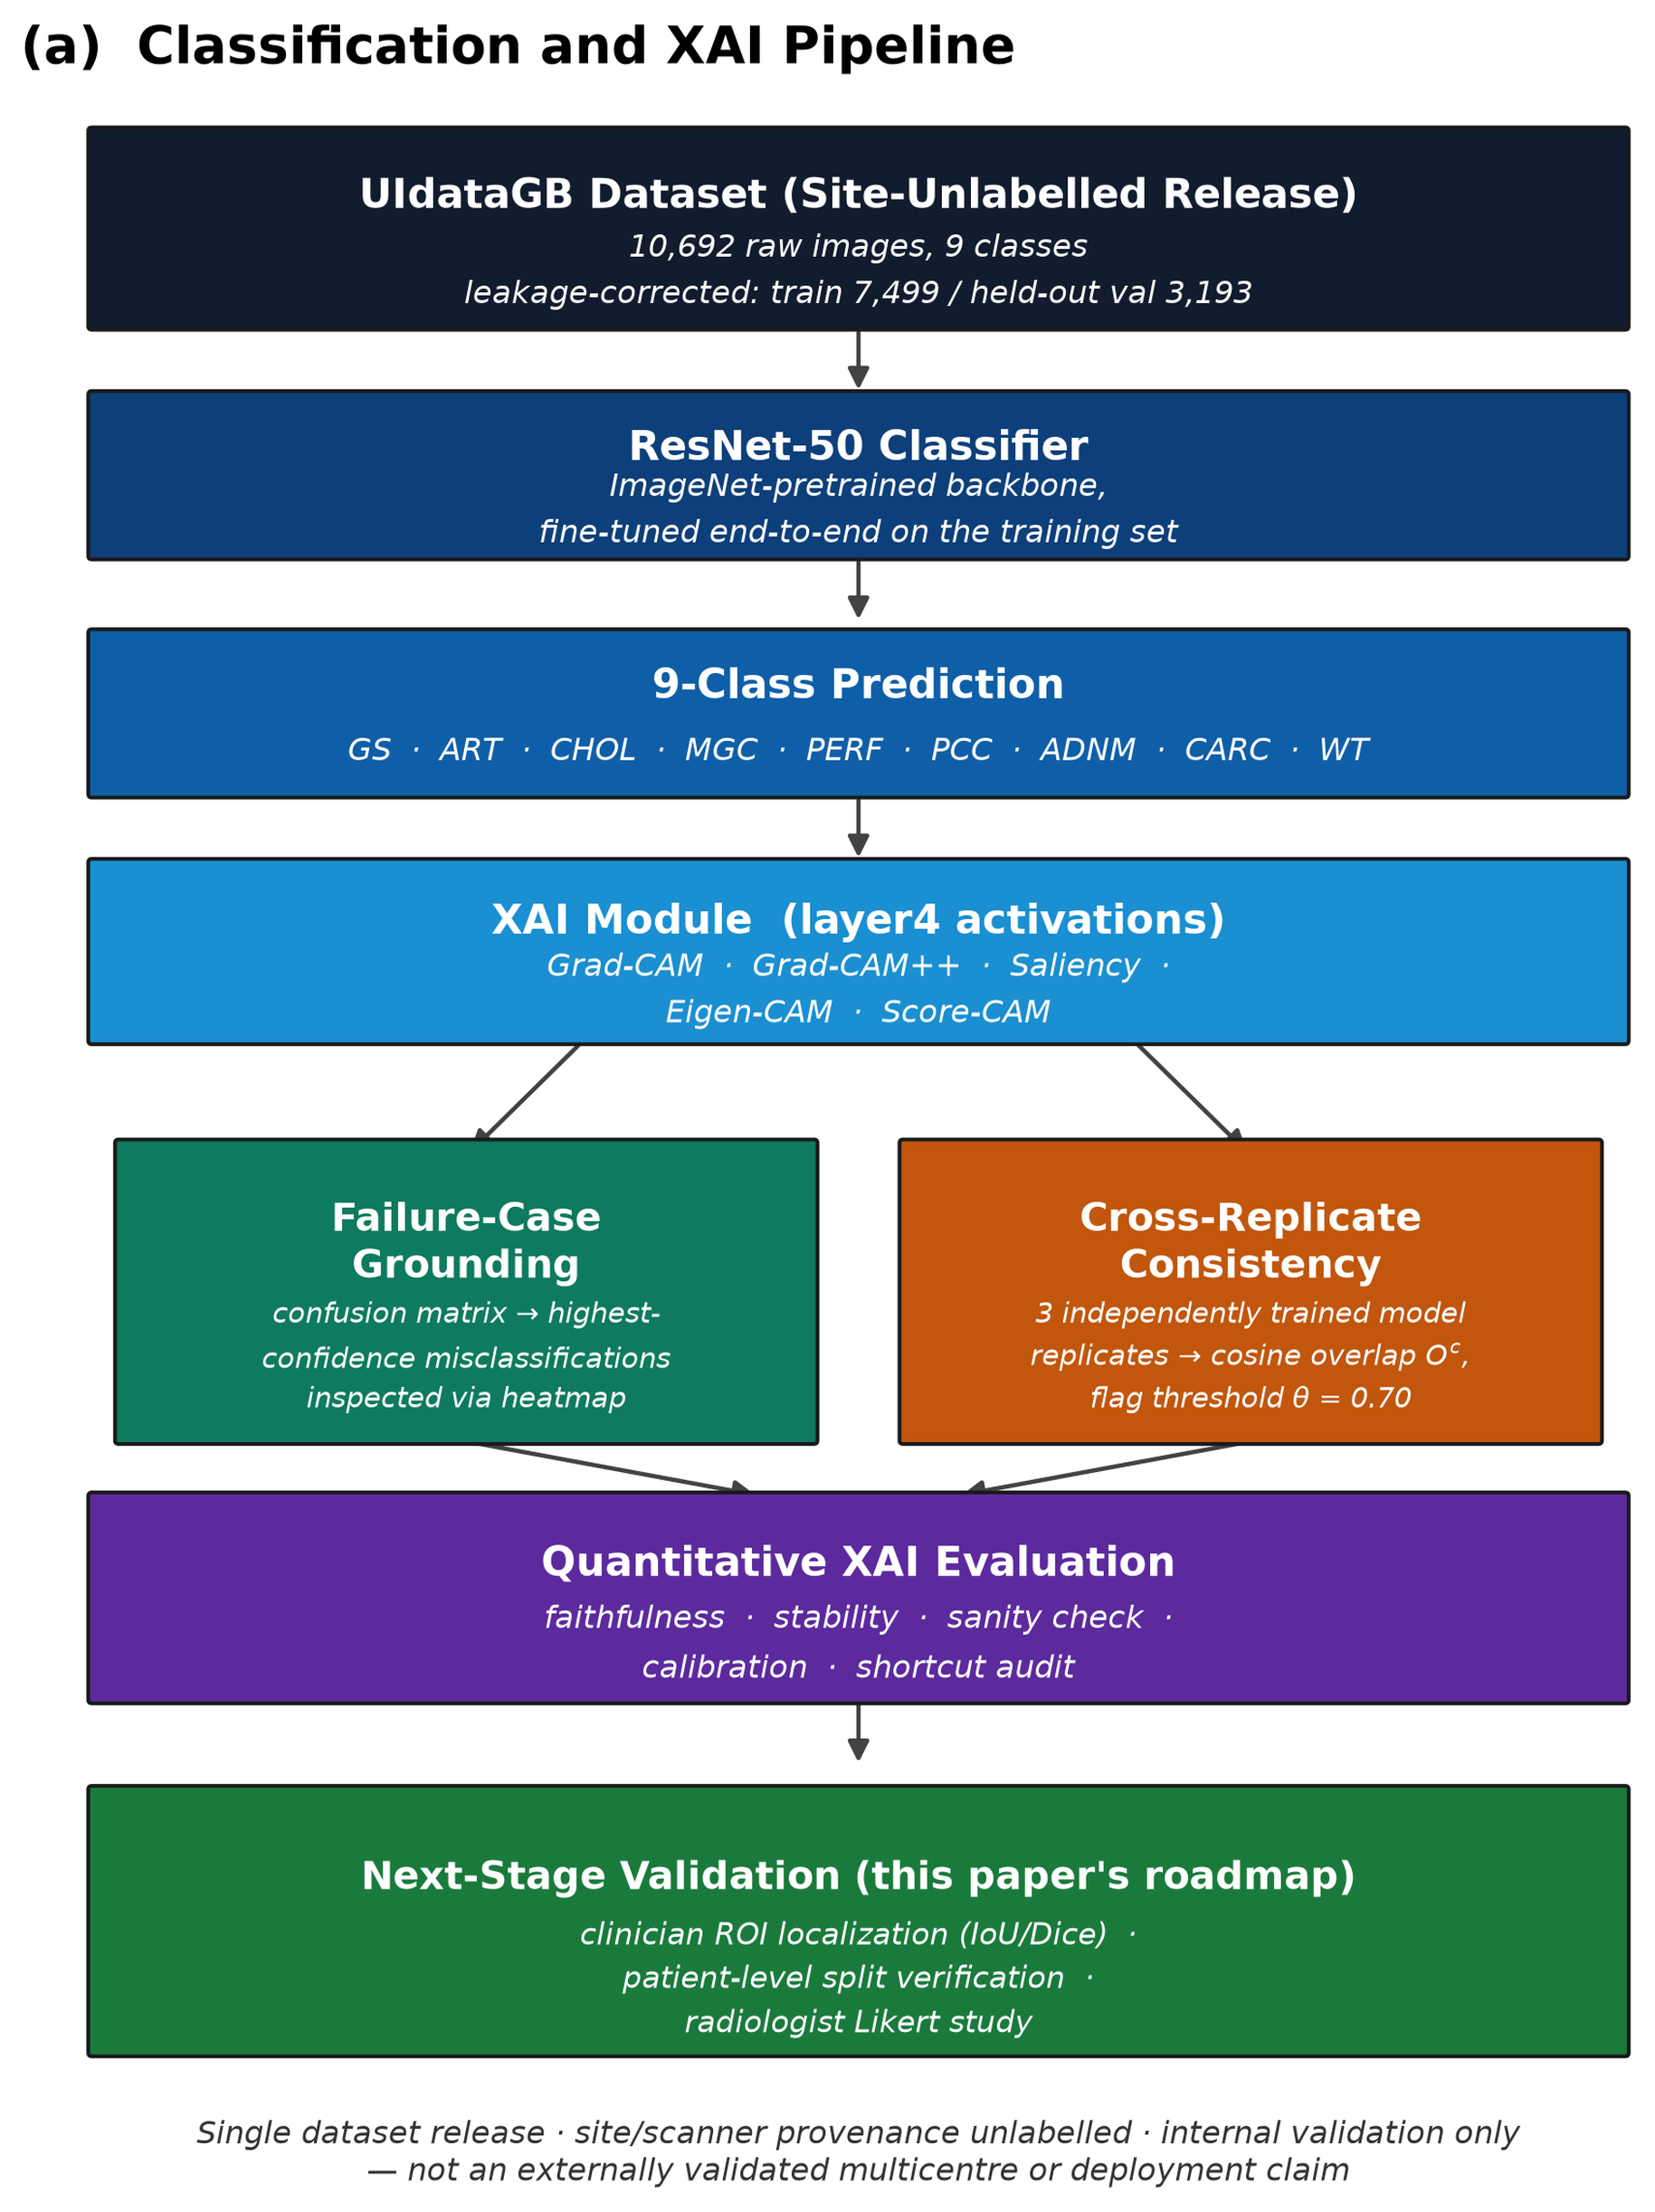
\includegraphics[width=0.92\linewidth]{figures/xai_pipeline_diagram_final}

\vspace{10pt}

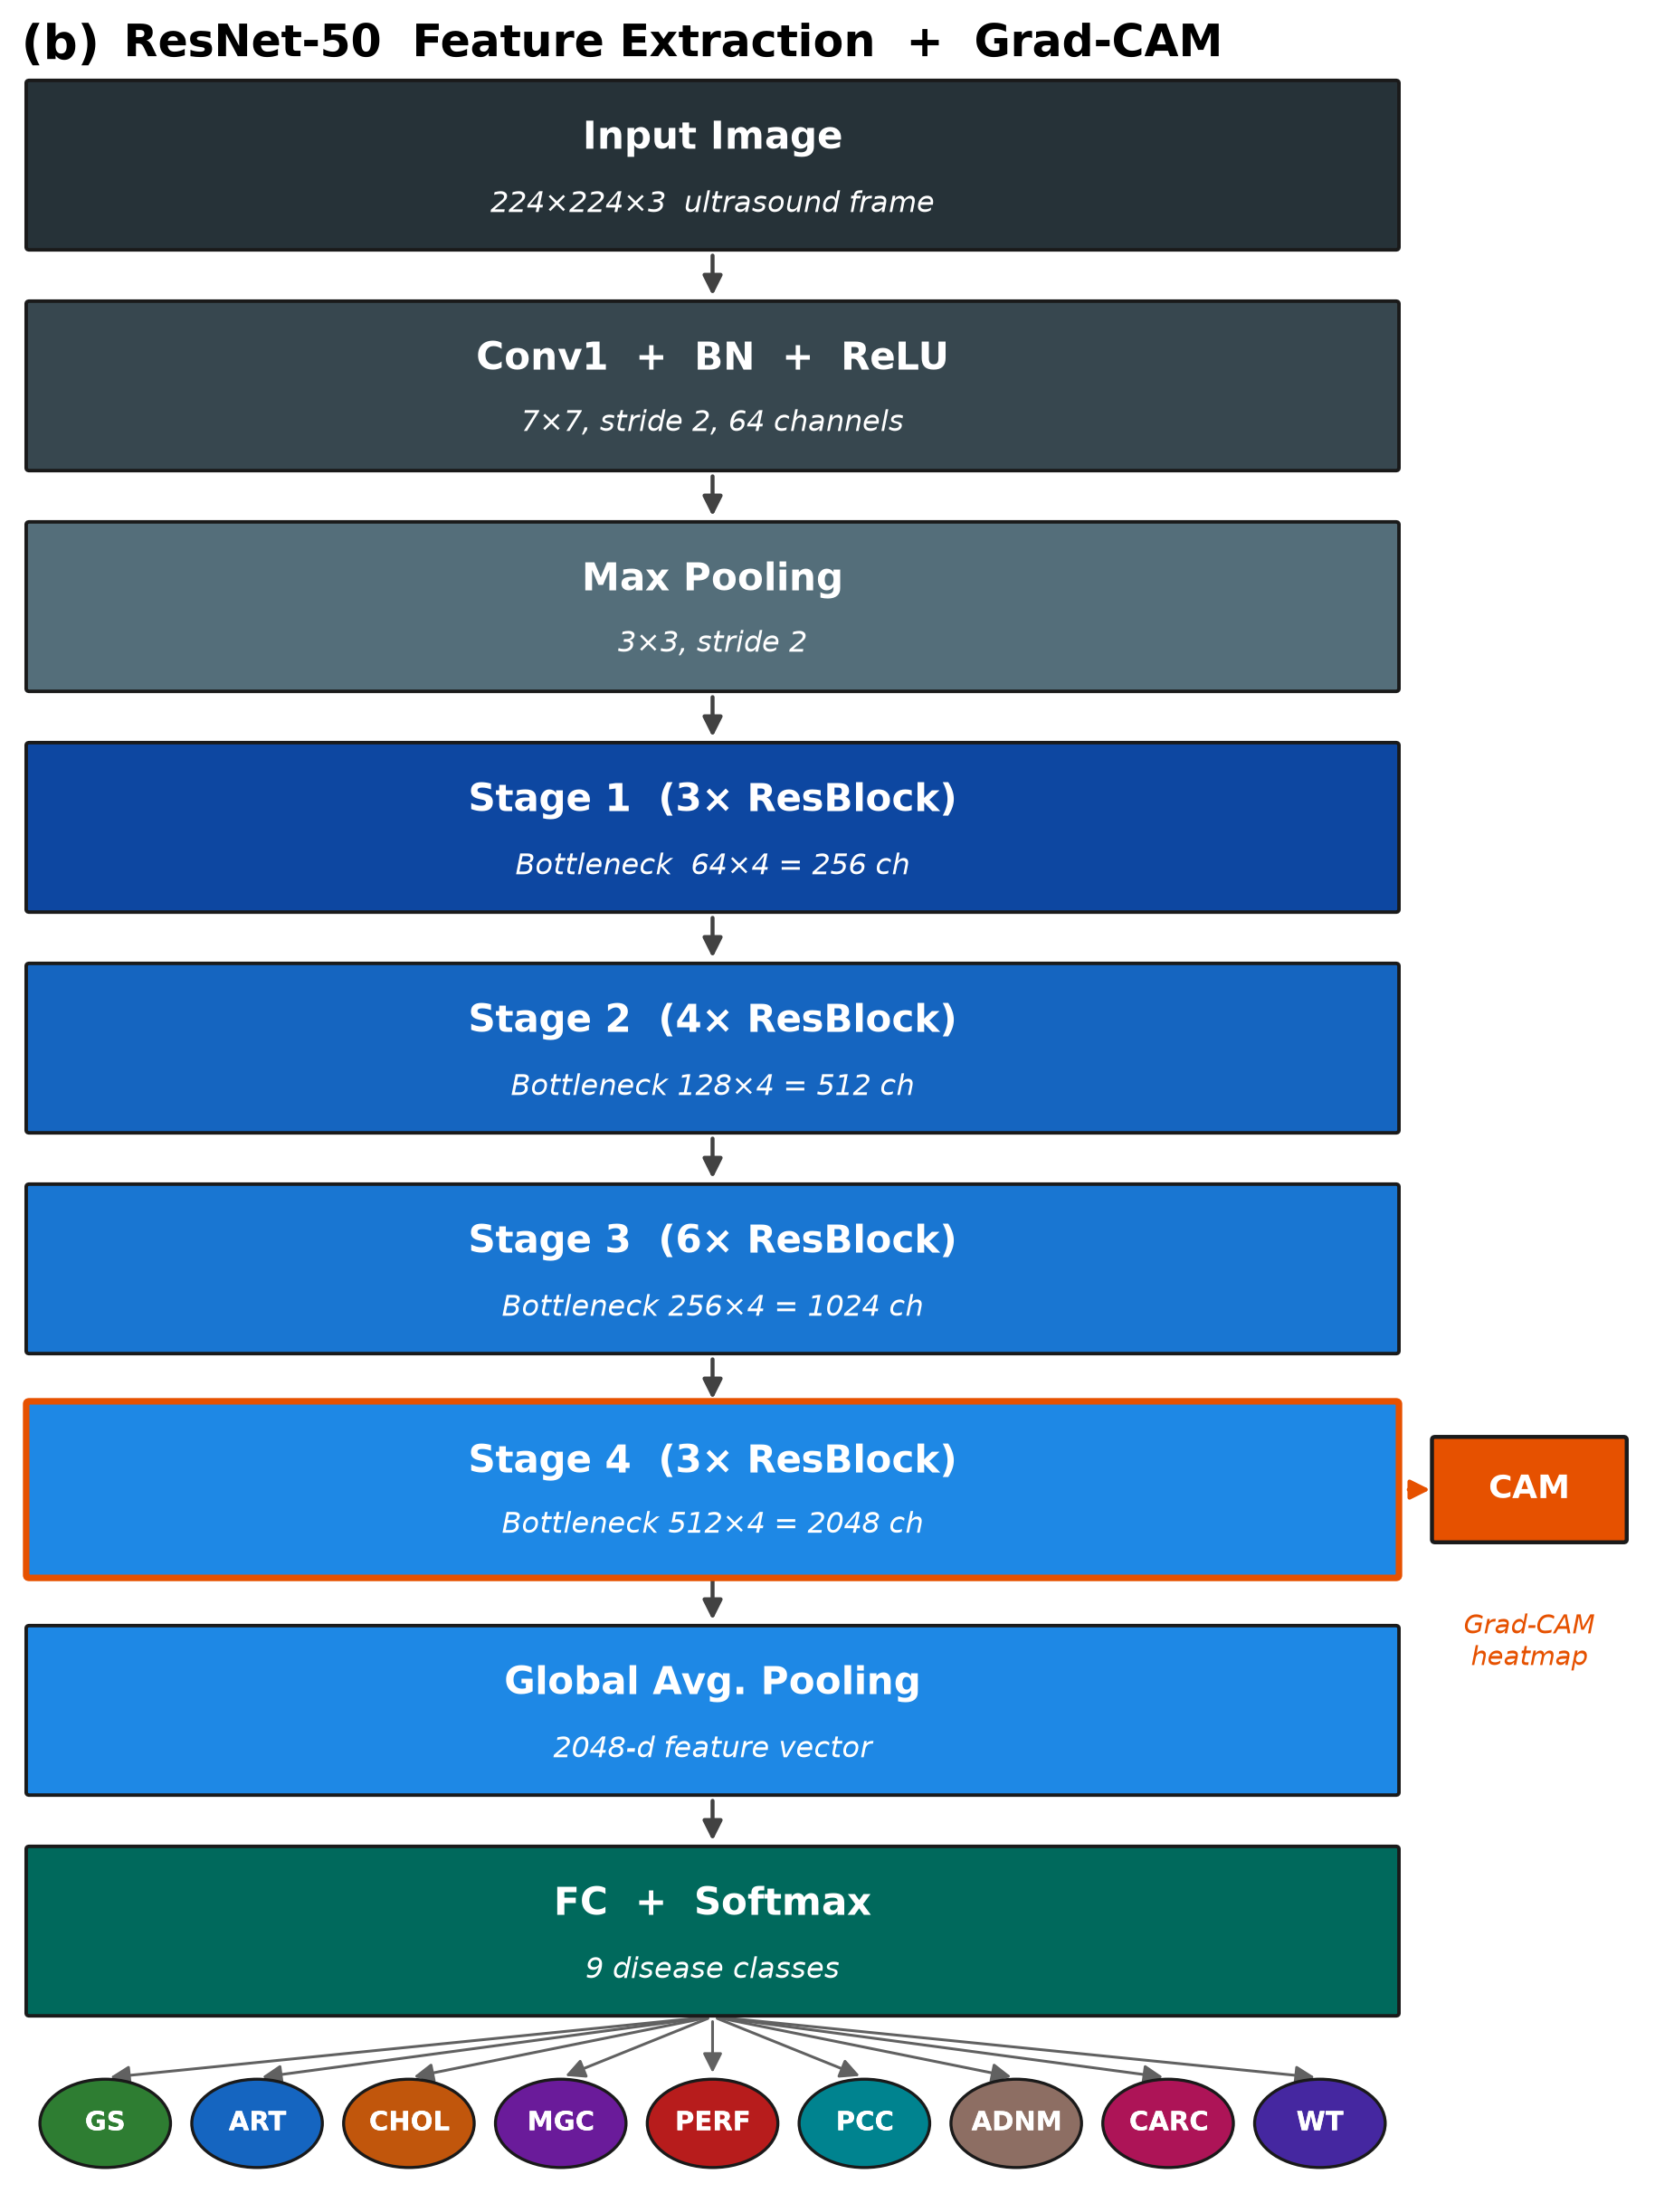
\includegraphics[width=0.92\linewidth]{figures/resnet_backbone_final}

\vspace{8pt}
\caption{(a)~End-to-end classification and XAI pipeline used in this paper, run on a site-unlabelled public dataset release. (b)~ResNet-50 backbone: all four CAM-family methods tap the Stage~4 (\texttt{layer4}) activations, the highest-level convolutional features before global average pooling. Both panels are rendered at identical scale for direct visual comparison.}
\label{fig:1}
\end{figure}

\subsection{Dataset description}

This study uses the publicly available UIdataGB dataset \cite{ref17}, a multi-class gallbladder ultrasound image collection spanning nine disease classes: Gallstones (GS), Abdomen \& Retroperitoneum (ART), Cholecystitis (CHOL), Membranous/Gangrenous Cholecystitis (MGC), Perforation (PERF), Polyps \& Cholesterol Crystals (PCC), Adenomyomatosis (ADNM), Carcinoma (CARC), and Wall Thickening (various causes, WT). Part of the collection was assembled from video-cine sequences, which can produce near-identical consecutive frames, so the released train/validation split was de-duplicated at the image-cluster level using perceptual hashing (64-bit pHash, Hamming distance~$\le 8$ treated as a near-duplicate) before any classification or XAI result was computed. That way, reported performance reflects genuine generalisation rather than memorised near-duplicates.

\textbf{Final dataset statistics.} The de-duplicated split comprises 7,499 training and 3,193 validation images (Table~\ref{tbl:1}, Fig.~\ref{fig:2}). Carcinoma is the largest class (1,590 images total) and Wall Thickening the smallest (990), but as Section~\ref{sec:results}.1 shows, the weakest-performing classes (Perforation, Gallstones) are not simply the smallest ones: class size alone does not explain the per-class performance profile.

\begin{table}[!ht]
\centering
\caption{UIdataGB Dataset Statistics: Class Distribution across Train / Validation Splits.}
\label{tbl:1}
\begin{tabular}{lccc}
\toprule
Class & Train & Validation & Total \\
\midrule
Gallstones (GS) & 927 & 399 & 1326 \\
Abdomen \& Retroperitoneum (ART) & 807 & 363 & 1170 \\
Cholecystitis (CHOL) & 795 & 351 & 1146 \\
Membranous/Gangrenous Cholecystitis (MGC) & 868 & 356 & 1224 \\
Perforation (PERF) & 742 & 320 & 1062 \\
Polyps \& Cholesterol Crystals (PCC) & 734 & 286 & 1020 \\
Adenomyomatosis (ADNM) & 813 & 351 & 1164 \\
Carcinoma (CARC) & 1120 & 470 & 1590 \\
Wall Thickening, various causes (WT) & 693 & 297 & 990 \\
\midrule
\textbf{Total} & \textbf{7499} & \textbf{3193} & \textbf{10692} \\
\bottomrule
\end{tabular}
\end{table}

\begin{figure*}[!ht]
\centering
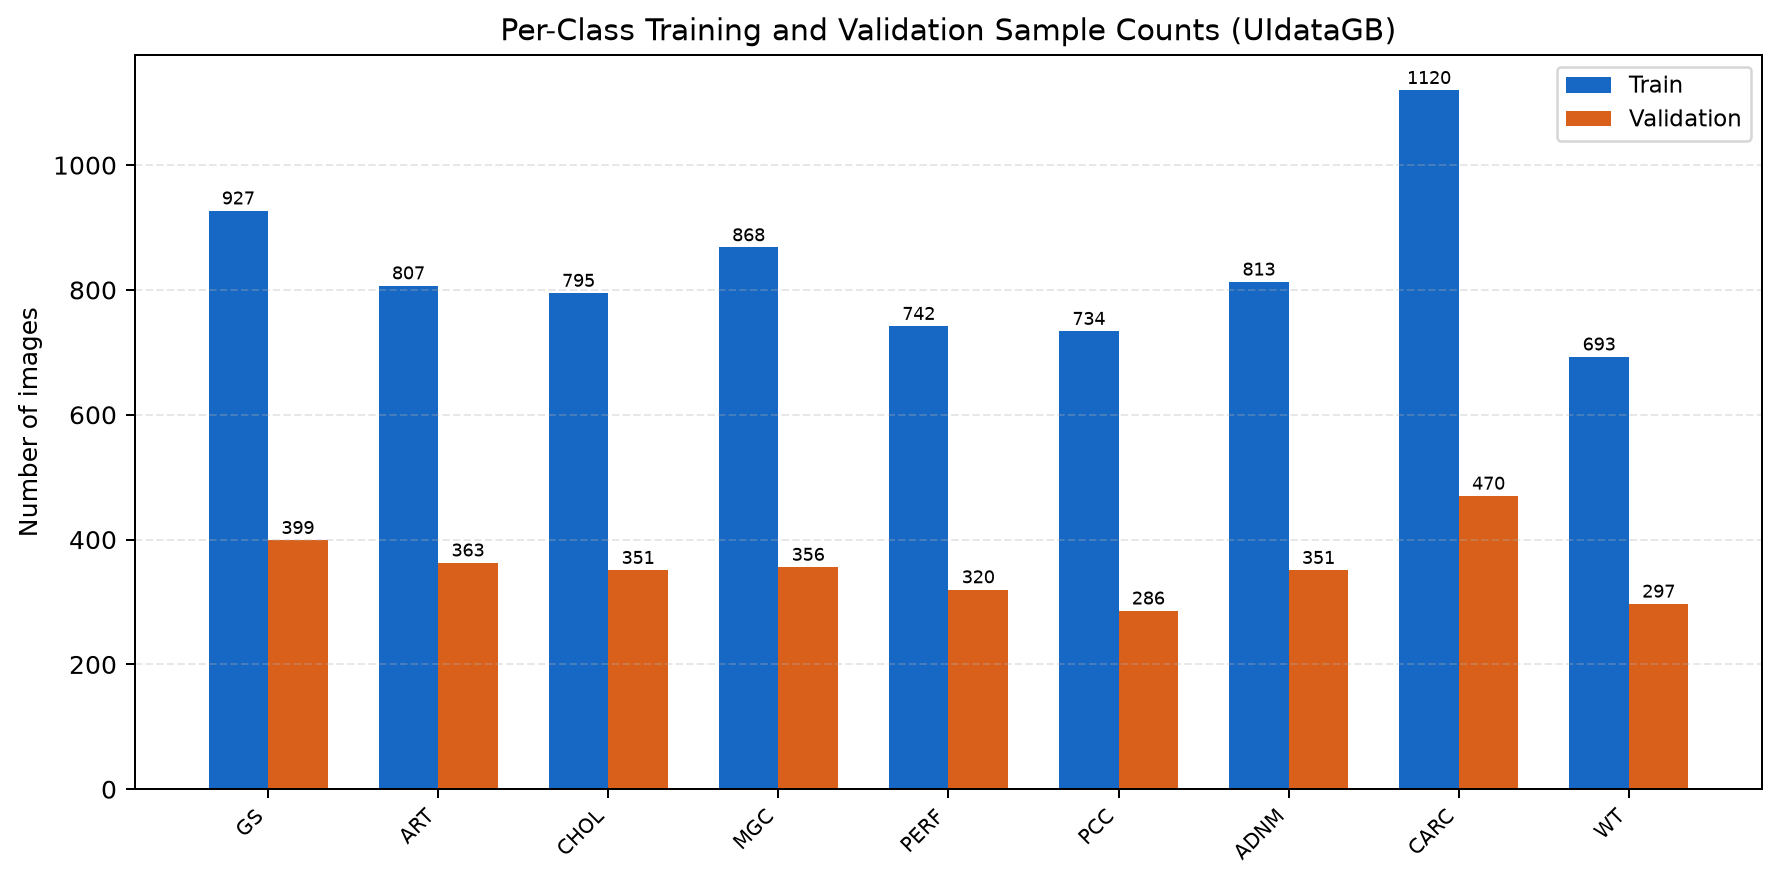
\includegraphics[width=0.75\textwidth]{figures/dataset_statistics.png}
\caption{Per-class training and validation sample counts (Table~\ref{tbl:1}). Carcinoma is the largest class (1,590 images); Wall Thickening is the smallest (990).}
\label{fig:2}
\end{figure*}

\subsection{Classification model and training configuration}

Images are resized to $224\times224$ and normalized using ImageNet statistics. Standard augmentations (random horizontal flip, $\pm15^\circ$ rotation, brightness/contrast jitter) \cite{ref43} are applied during training only, not at validation time, and standard cross-entropy is used (Table~\ref{tbl:2}) rather than a class-imbalance-aware loss such as focal loss \cite{ref44}. A weighted or focal-loss ablation is a natural next step given the class imbalance in Table~\ref{tbl:1}, and is left for future work.

ResNet-50 \cite{ref27} pretrained on ImageNet \cite{ref30} is adopted as the feature extractor, with the final fully-connected layer replaced by a nine-class classification head: Dropout($p=0.4$)~$\rightarrow$~Dense(256, ReLU)~$\rightarrow$~Dropout($p=0.3$)~$\rightarrow$~Dense(9). The head outputs raw logits over the nine classes of Table~\ref{tbl:1}. Training uses \texttt{nn.CrossEntropyLoss} (Table~\ref{tbl:2}), which expects raw logits and applies log-softmax internally, while softmax is applied only at inference time to obtain the reported probabilities and confidence values (Section~\ref{sec:results}.4); no softmax layer is part of the trained model itself. ResNet-50's residual structure and deep feature hierarchy make it well suited to CAM-family explanation methods, since the \texttt{layer4} output encodes rich semantic features prior to global average pooling. It was chosen over deeper or more parameter-efficient alternatives such as DenseNet-121 \cite{ref28} or EfficientNet \cite{ref29} mainly for comparability with prior gallbladder-ultrasound baselines \cite{ref7}, which are themselves ResNet-based; comparing backbones is not this paper's focus.

\begin{table}[!ht]
\centering
\caption{Hyperparameter and Training Configuration.}
\label{tbl:2}
\begin{tabular}{ll}
\toprule
Hyperparameter & Value \\
\midrule
Backbone & ResNet-50 (ImageNet) \\
Optimizer & Adam, $\beta_1{=}0.9$ \\
Learning rate & $1\times10^{-4}$ \\
Weight decay & $1\times10^{-4}$ \\
Loss function & Cross-entropy \\
Batch size & 32 \\
Training epochs & 10 \\
Replicate models $R$ & 3 \\
Train / Val split & 70\% / 30\% (cluster-level, Section~\ref{sec:methods}.1) \\
Framework & PyTorch~2.x, torchvision~0.15 \\
Model parameters & 24.03M (all trainable) \\
Checkpoint size & 96~MB (fp32) \\
Inference latency & 187~ms/image (CPU, 4 threads); ${\sim}44$~ms (GTX~1050) \\
\bottomrule
\end{tabular}

\vspace{2pt}
\raggedright\footnotesize Latency is architecture-bound, not class-count-bound (a 9-way vs. 5-way softmax head differs by a negligible 2,048$\times$4 parameters), so the measured value from the identical ResNet-50/GTX~1050 setup is unchanged.
\end{table}

\subsection{Explainability methods and consistency metric}

Five complementary visual-explanation methods are applied to the trained ResNet-50 model. Four of them target the final convolutional layer (\texttt{layer4}), which encodes the highest-level semantic features before global average pooling, while the fifth (Saliency) operates directly in pixel space. Let $A^k \in \mathbb{R}^{H \times W}$ denote the $k$-th feature map of the target layer, and let $y^c$ be the class score for class $c$ before softmax.

\textbf{1)~Grad-CAM:} Grad-CAM \cite{ref11} computes a class-discriminative localization map by weighting each feature map $A^k$ with the global-average-pooled gradient of $y^c$ with respect to that map:
\begin{equation}
\alpha_k^c = \frac{1}{Z}\sum_i\sum_j \frac{\partial y^c}{\partial A^k_{ij}},
\end{equation}
\begin{equation}
L^c_{\text{GradCAM}} = \mathrm{ReLU}\!\left(\sum_k \alpha_k^c A^k\right).
\end{equation}
The ReLU discards negative activations, retaining only positive evidence. The resulting heatmap is upsampled to $224\times224$ and overlaid on the input image.

\textbf{2)~Grad-CAM++:} Grad-CAM++ \cite{ref12} extends Grad-CAM using a pixel-wise weighted average of second-order partial derivatives, giving more weight to pixels where the gradient is strong and locally peaked, producing sharper localization for small or multiple lesions:
\begin{equation}
\alpha_k^{c,++} = \sum_{i,j} \frac{(\partial^2 y^c / \partial (A^k_{ij})^2)}{2(\partial^2 y^c / \partial (A^k_{ij})^2) + \sum_{a,b} A^k_{ab}\,(\partial^3 y^c / \partial (A^k_{ij})^3)},
\end{equation}
\begin{equation}
L^c_{\text{GradCAM++}} = \mathrm{ReLU}\!\left(\sum_k \alpha_k^{c,++} A^k\right).
\end{equation}
\textit{Equation--implementation cross-check:} this presentation follows the pixel-wise weighting structure of Chattopadhay et~al.~\cite{ref12}; before this manuscript is finalised, both the equation above and the \texttt{gradcam.py} implementation should be checked line-by-line against the original paper's Eq.~(4)--(19) to confirm no compression or transcription error, since the two must match exactly for the reported results to be reproducible from the stated formula.

\textbf{3)~Saliency Maps:} Gradient saliency \cite{ref33} computes the gradient of the class score $y^c$ with respect to the input image pixels $\mathbf{x} \in \mathbb{R}^{3 \times H \times W}$:
\begin{equation}
S^c = \left|\frac{\partial y^c}{\partial \mathbf{x}}\right|.
\end{equation}
This highlights pixel-level evidence in input space rather than feature-map space. It is noisier than Grad-CAM, but requires no target-layer choice and captures fine-grained texture cues, and it still requires differentiable, white-box access to the model's gradients: architecture-agnostic in that it needs no CAM-style layer tap, but not model-agnostic in the stricter input/output-only sense of methods such as LIME or SHAP. For visualisation, the maximum over colour channels is taken and Gaussian smoothing applied ($\sigma=1$).

\textbf{4)~Eigen-CAM:} Eigen-CAM \cite{ref34} is class-agnostic: it reshapes the target-layer activation tensor $A \in \mathbb{R}^{K \times HW}$ and computes its dominant direction of variation via singular value decomposition, $A = U\Sigma V^{\!\top}$, projecting onto the first principal component to obtain an $HW$-dimensional saliency map reshaped back to $H \times W$. Because Eigen-CAM does not condition on class $c$, it highlights the single dominant activation pattern in the layer regardless of the predicted class. This makes it useful as a lightweight, gradient-free baseline, but with weaker class-discriminative power than the methods above. \textit{Equation--implementation cross-check:} the exact projection expression and matrix orientation above should be verified against Muhammad and Yeasin's original formulation~\cite{ref34} and the \texttt{gradcam.py} implementation before this manuscript is finalised, to confirm the dimensions of $A$, $U$, $\Sigma$, $V$ are stated consistently throughout.

\textbf{5)~Score-CAM:} Score-CAM \cite{ref35} is gradient-free: each channel's importance weight is obtained by masking the input image with that channel's (upsampled, normalised) activation map and measuring the resulting change in the model's own softmax score for class $c$,
\begin{equation}
\alpha_k^{c,\text{score}} = f^c\big(\mathbf{x}\odot \text{Up}(A^k)\big) - f^c(\mathbf{x}_b),
\end{equation}
\begin{equation}
L^c_{\text{ScoreCAM}} = \mathrm{ReLU}\!\left(\sum_k \alpha_k^{c,\text{score}} A^k\right),
\end{equation}
where $f^c(\cdot)$ is the softmax score for class $c$ and $\mathbf{x}_b$ a baseline (blank) input. Because the weighting is derived directly from the model's forward-pass behaviour rather than from gradients, Score-CAM avoids gradient saturation and noise, at the cost of one forward pass per channel (computed here on GPU).

After training, all five methods above are applied to the primary model $M_0$ and to each of the three replicate models $\{M_1,M_2,M_3\}$ (Section~\ref{sec:methods}.3), using the same input images, which allows consistency scores to be computed for every class and method. Algorithm~\ref{alg:1} formalises the pipeline.

\begin{algorithm}[tb]
\caption{XAI Pipeline with Consistency Scoring}
\label{alg:1}
\begin{algorithmic}[1]
\Require primary model $M_0$, replicate models $\{M_r\}_{r=1}^{3}$, test image $\mathbf{x}$, class set $\mathcal{C} = \{$GS, ART, CHOL, MGC, PERF, PCC, ADNM, CARC, WT$\}$, target conv layer $\ell^*$, threshold $\theta$
\Ensure heatmaps per method and model, consistency scores $O_r^c$
\For{method $m \in \{$GradCAM, GradCAM++, Saliency, EigenCAM, ScoreCAM$\}$}
  \For{$c \in \mathcal{C}$}
    \State $L^c_{\text{primary}} \leftarrow \text{XAI}_m(\mathbf{x};\,M_0,\,c,\,\ell^*)$
    \State Upsample $L^c_{\text{primary}}$ to $224{\times}224$; overlay on $\mathbf{x}$
    \For{each replicate $r \in \{1,2,3\}$}
      \State $L^c_r \leftarrow \text{XAI}_m(\mathbf{x};\,M_r,\,c,\,\ell^*)$
      \State $O_r^c \leftarrow \dfrac{\langle L^c_{\text{primary}},\,L^c_r\rangle}{\|L^c_{\text{primary}}\|\cdot\|L^c_r\|}$
      \If{$O_r^c < \theta$}
        \State flag as explanation-divergent
      \EndIf
    \EndFor
  \EndFor
\EndFor
\State \Return all heatmaps, $\{O_r^c\}$ per method
\end{algorithmic}
\end{algorithm}

A heatmap that looks anatomically plausible for one trained model is not, by itself, evidence that the explanation reflects a stable property of the learned decision boundary rather than an artifact of that specific training run. To test this, a cosine-consistency score is defined between the primary model's heatmap and each of $R{=}3$ independently trained replicate models' heatmaps, for the same class and image:
\begin{equation}
O_r^c = \frac{\langle L^c_{\text{primary}},\, L^c_r \rangle}{\|L^c_{\text{primary}}\| \cdot \|L^c_r\|},\qquad r=1,\dots,R,
\end{equation}
where both heatmaps are flattened and normalised to $[0,1]$ before computing cosine similarity. Because $O_r^c \in [0,1]$, a value near 1 means the two independently trained models produce essentially the same explanation for class $c$, while a value near 0 means the explanation is training-run dependent rather than a robust model property. A threshold of $\theta = 0.70$ flags class/replicate pairs whose explanations diverge substantially, though this threshold is operational and exploratory rather than an established, validated cut-off for explanation agreement: no clinical or XAI-specific validation of a universal 0.70 threshold is known to the authors, and it is the continuous similarity score, not the binary flag, that is treated as the primary quantity throughout Section~\ref{sec:results}.3.

All classification results in Section~\ref{sec:results}.1 come from one primary model, $M_0$, trained on the full 7,499-image corrected training set with no resampling. To compute $O^c$, three additional replicate models $\{M_1,M_2,M_3\}$ are trained on three disjoint subsets of that same corrected training set (2,749, 2,089, and 2,661 images respectively); these are training-resampling replicates, not independent clinical sites. Each subset has a different per-class composition by construction, so $O^c$ jointly probes robustness to both re-initialisation and moderate class-distribution shift. Running all five XAI methods on four models over the full 3,193-image validation set is computationally expensive, so $O^c$ is instead computed on a stratified subset of 8 images per class (72 total); the faithfulness, stability, and sanity-check batteries of Section~\ref{sec:results}.4 use larger stratified samples of 144, 216, and 108 images respectively. This remains a reproducibility check on the explanation, not a multicentre or domain-shift experiment. Genuine cross-site validation instead requires images with known, traceable hospital or scanner identity, which this dataset's public release does not provide (Section~\ref{sec:limitations}, Section~\ref{sec:future-research}).

\subsection{Evaluation protocol}

\textbf{1)~Classification Metrics:} Classification performance is reported as Accuracy, Macro-F1, AUC-ROC (one-vs-rest) \cite{ref45}, and per-class Sensitivity and Specificity. Given the class imbalance in Table~\ref{tbl:1}, ROC-AUC should be read alongside per-class sensitivity rather than in isolation, since precision-recall curves can be more informative for rarer classes under imbalance \cite{ref46}; it is retained mainly for continuity with prior gallbladder-ultrasound baselines \cite{ref7}, \cite{ref19}, \cite{ref20}, \cite{ref21}. Per-class F1 and AUC (Table~\ref{tbl:4}) provide the classification context within which XAI results should be interpreted, and classes with low F1 (Perforation, Gallstones) are the primary targets for XAI investigation.

\textbf{2)~XAI Evaluation Metrics:} XAI quality is evaluated along seven dimensions: (1)~\textbf{anatomical plausibility}, a visual check of whether heatmaps concentrate on gallbladder wall, lumen, and adjacent tissue rather than artefacts (Section~\ref{sec:results}.3); (2)~\textbf{cross-method comparison}, both qualitative and quantitative, across all five methods (Section~\ref{sec:results}.3); (3)~\textbf{cross-replicate consistency}, the $O^c$ score of Section~\ref{sec:methods}.3, with $\theta=0.70$ as the divergence threshold (Section~\ref{sec:results}.3); (4)~\textbf{faithfulness}, via deletion/insertion curves against a random control (Section~\ref{sec:results}.4); (5)~\textbf{stability}, the explanation's agreement under clinically invariant transforms (Section~\ref{sec:results}.4); (6)~a \textbf{model-randomization sanity check} (Section~\ref{sec:results}.4); and (7)~a \textbf{shortcut-learning audit} (Section~\ref{sec:results}.4). SSIM, Pearson correlation, and top-decile IoU quantify agreement in (5), and deletion/insertion AUC quantifies (4). The one dimension this paper does \textit{not} establish is localization of the explanation against clinician-annotated regions of interest, which needs expert annotation and is scoped as the immediate next step (Section~\ref{sec:future-research}).

A classifier can be accurate yet miscalibrated, since its softmax confidence need not match its true correctness rate \cite{ref42}. A single scalar temperature $T>0$ is therefore fit post-hoc on a held-out calibration split, dividing the model's pre-softmax logits $\mathbf{z}$ by $T$ before the softmax, $\hat{p} = \mathrm{softmax}(\mathbf{z}/T)$, chosen to minimise negative log-likelihood without altering predictions (argmax is invariant to $T$). Expected Calibration Error (ECE, 15 bins) and Brier score are reported both before and after temperature scaling (Section~\ref{sec:results}.4).

All experiments and XAI analyses were run with a fixed random seed (seed~=~42 for the primary model, seeds~7 and 123 for the multi-seed replication of Table~\ref{tbl:3}) for reproducibility, in a software environment of Python~3.10, PyTorch~2.x, and torchvision~0.15. The de-duplication split correction (Section~\ref{sec:methods}.1) uses 64-bit perceptual hashing via the \texttt{imagehash} library and a union-find connected-components implementation, included in \texttt{fedgb/dedupe\_split\_uidatagb.py}. XAI heatmaps are generated post-training using the saved model checkpoints, with full code---including all five XAI methods and the consistency-scoring module---included in \texttt{fedgb/gradcam.py}. The UIdataGB dataset is publicly available via its Data in Brief release \cite{ref17}.

\section{Results and Analysis}
\label{sec:results}

This section presents overall and per-class classification performance (Section~\ref{sec:methods}.1), a grounded failure-case analysis, a comparative heatmap analysis across all five methods, and quantitative results for cross-replicate explanation consistency, faithfulness, stability, sanity checking, calibration, and shortcut auditing.

\subsection{Classification performance}

Classification performance is reported for the primary-model configuration (Table~\ref{tbl:2}) on the held-out validation split described in Section~\ref{sec:methods}.1.

\begin{table}[!ht]
\centering
\caption{Overall Classification Performance, Primary-Model Configuration (seed~=~42).}
\label{tbl:3}
\begin{tabular}{lc}
\toprule
Metric & Value \\
\midrule
Accuracy & \textbf{0.9305} \\
Macro-F1 & \textbf{0.9303} \\
Macro AUC-ROC & \textbf{0.9965} \\
Validation $n$ & 3193 \\
\bottomrule
\end{tabular}

\vspace{2pt}
\raggedright\footnotesize A three-seed replication (seeds~7, 42, 123; identical architecture, optimizer, and epoch budget) gives accuracy~$0.9210\pm0.0131$, macro-F1~$0.9207\pm0.0131$, macro AUC-ROC~$0.9948\pm0.0023$ (mean~$\pm$~std, $n=3$).
\end{table}

\textbf{Paired statistical significance, three-seed replication.} McNemar's exact test \cite{ref49} on paired per-image accuracy is the primary significance test here, since it directly compares two classifiers' predictions on the same held-out images: the seed~7-vs-seed~42 difference (0.9264 vs.\ 0.9305) is \textit{not} significant ($p=0.451$), while both comparisons involving seed~123 are ($p<0.001$ each, uncorrected for the 3 pairwise seed comparisons tested). DeLong's test \cite{ref47} was also run on per-class, one-vs-rest AUC (1 of 9 classes differs significantly between seed~7 and seed~42, versus 5 of 9 for each comparison involving seed~123, again uncorrected across the resulting 9-class~$\times$~3-seed-pair family of tests) and points in the same qualitative direction, but DeLong's test is designed to compare two correlated ROC curves evaluated on identical patients, not two independently trained models' predictions on the same image set; it is reported here as a secondary, exploratory check rather than the basis for any claim, precisely because that assumption does not hold across independently seeded training runs. Bootstrap 95\% confidence intervals \cite{ref48} (2,000 resamples) come out as seed~7: accuracy $[0.917,\,0.935]$; seed~42: $[0.922,\,0.939]$; seed~123: $[0.895,\,0.915]$; seed~123's interval does not overlap the other two. With only three seeds, however, this is not enough to establish a seed-to-seed distribution or to distinguish a genuinely weaker training run from an unlucky but otherwise typical one; the more defensible claim is only that seed~123 performs measurably worse than the other two \textit{on this specific comparison}, not that it is characteristically different in some reproducible way, and the three-seed mean (92.10\%) should be read alongside all three individual values rather than as a stable population estimate. A separate check asks whether those image-level bootstrap intervals themselves understate uncertainty. Because images sharing a filename-prefix group are correlated rather than independent, a \textit{group} bootstrap (resampling whole filename-prefix groups with replacement, $n=209$ groups over 3,193 validation images, 2,000 resamples) was run alongside the image-level one for all three seeds. The group-aware 95\% accuracy interval comes out 2.7--2.9$\times$ wider than the image-level interval at every seed (seed~7: width 0.018~$\rightarrow$~0.051; seed~42: 0.017~$\rightarrow$~0.046; seed~123: 0.020~$\rightarrow$~0.054), confirming that treating within-group images as independent observations meaningfully understates true uncertainty. The same procedure also reports macro PR-AUC (0.968--0.981) and balanced accuracy (0.909--0.929) per seed, both omitted from the original battery (\texttt{outputs/phase0/group\_aware\_statistics.json}); this is a diagnostic on interval width, not a claim that the point estimates themselves are otherwise incorrect.

Table~\ref{tbl:4} reports the primary model's per-class performance on the held-out validation set (seed~=~42). Unlike the GBCU single-centre dataset examined in prior work (Section~\ref{sec:related-work}), per-class F1 here does not track training-set size closely: the two weakest classes, Perforation (F1~=~0.8944) and Gallstones (F1~=~0.9001), are mid-sized (1,062 and 1,326 total images respectively), while the smallest class, Wall Thickening (990 images), reaches a comfortably higher F1 of 0.9406. These two weakest classes are the primary targets for the failure-case and XAI analysis below.

\begin{table*}[!ht]
\centering
\caption{Per-Class Performance of the Primary Model (9-Class UIdataGB). Classes with low F1 are the primary XAI targets. Best F1/AUC in bold.}
\label{tbl:4}
\begin{tabular}{lcccc}
\toprule
Class & F1 & AUC-ROC & Sensitivity & Specificity \\
\midrule
Gallstones (GS) & 0.9001 & 0.9955 & 0.9373 & 0.9792 \\
Abdomen \& Retroperitoneum (ART) & 0.9161 & 0.9911 & 0.8871 & 0.9936 \\
Cholecystitis (CHOL) & \textbf{0.9601} & 0.9985 & 0.9259 & 0.9996 \\
Membranous/Gangrenous Cholecystitis (MGC) & 0.9428 & 0.9984 & 0.9494 & 0.9919 \\
Perforation (PERF) & 0.8944 & 0.9952 & 0.8469 & 0.9948 \\
Polyps \& Cholesterol Crystals (PCC) & 0.9375 & 0.9958 & 0.8916 & 0.9990 \\
Adenomyomatosis (ADNM) & 0.9360 & 0.9990 & \textbf{1.0000} & 0.9831 \\
Carcinoma (CARC) & 0.9455 & 0.9956 & 0.9404 & 0.9916 \\
Wall Thickening (WT) & 0.9406 & \textbf{0.9996} & 0.9865 & 0.9886 \\
\midrule
\textbf{Macro Avg} & \textbf{0.9303} & \textbf{0.9965} & 0.9295 & 0.9913 \\
\bottomrule
\end{tabular}
\end{table*}

\begin{figure*}[!ht]
\centering
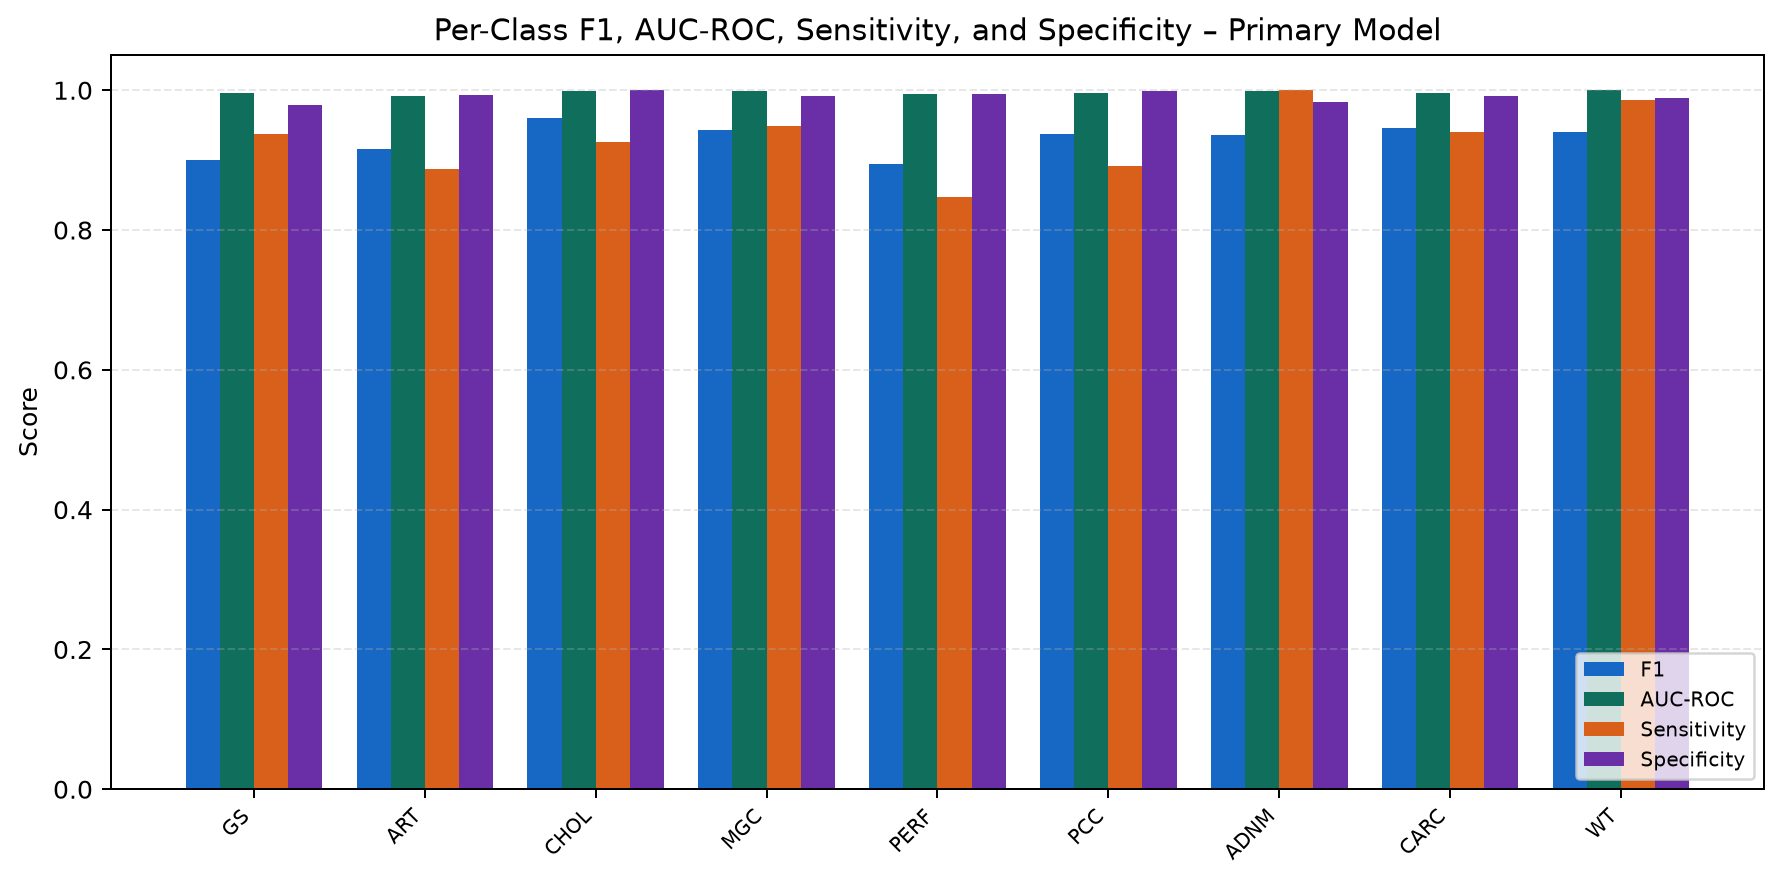
\includegraphics[width=0.75\textwidth]{figures/per_class_metrics.png}
\caption{Per-class F1, AUC-ROC, Sensitivity, and Specificity for the primary model. All nine classes exceed F1~0.89; Perforation and Gallstones are the most challenging by F1, driven by specific confusion pairs (Section~\ref{sec:results}.2) rather than small class size.}
\label{fig:3}
\end{figure*}

\textit{XAI Finding (1):} The per-class performance profile directly informs XAI priorities. Cholecystitis (F1~=~0.9601) and Wall Thickening (AUC~=~0.9996) are the strongest classes and serve as positive controls for anatomical plausibility. Perforation (F1~=~0.8944, sensitivity~0.8469) and Gallstones (F1~=~0.9001) are the most difficult classes---their heatmaps are examined below for whether errors correlate with attention on incorrect anatomical regions.

\begin{figure*}[!ht]
\centering
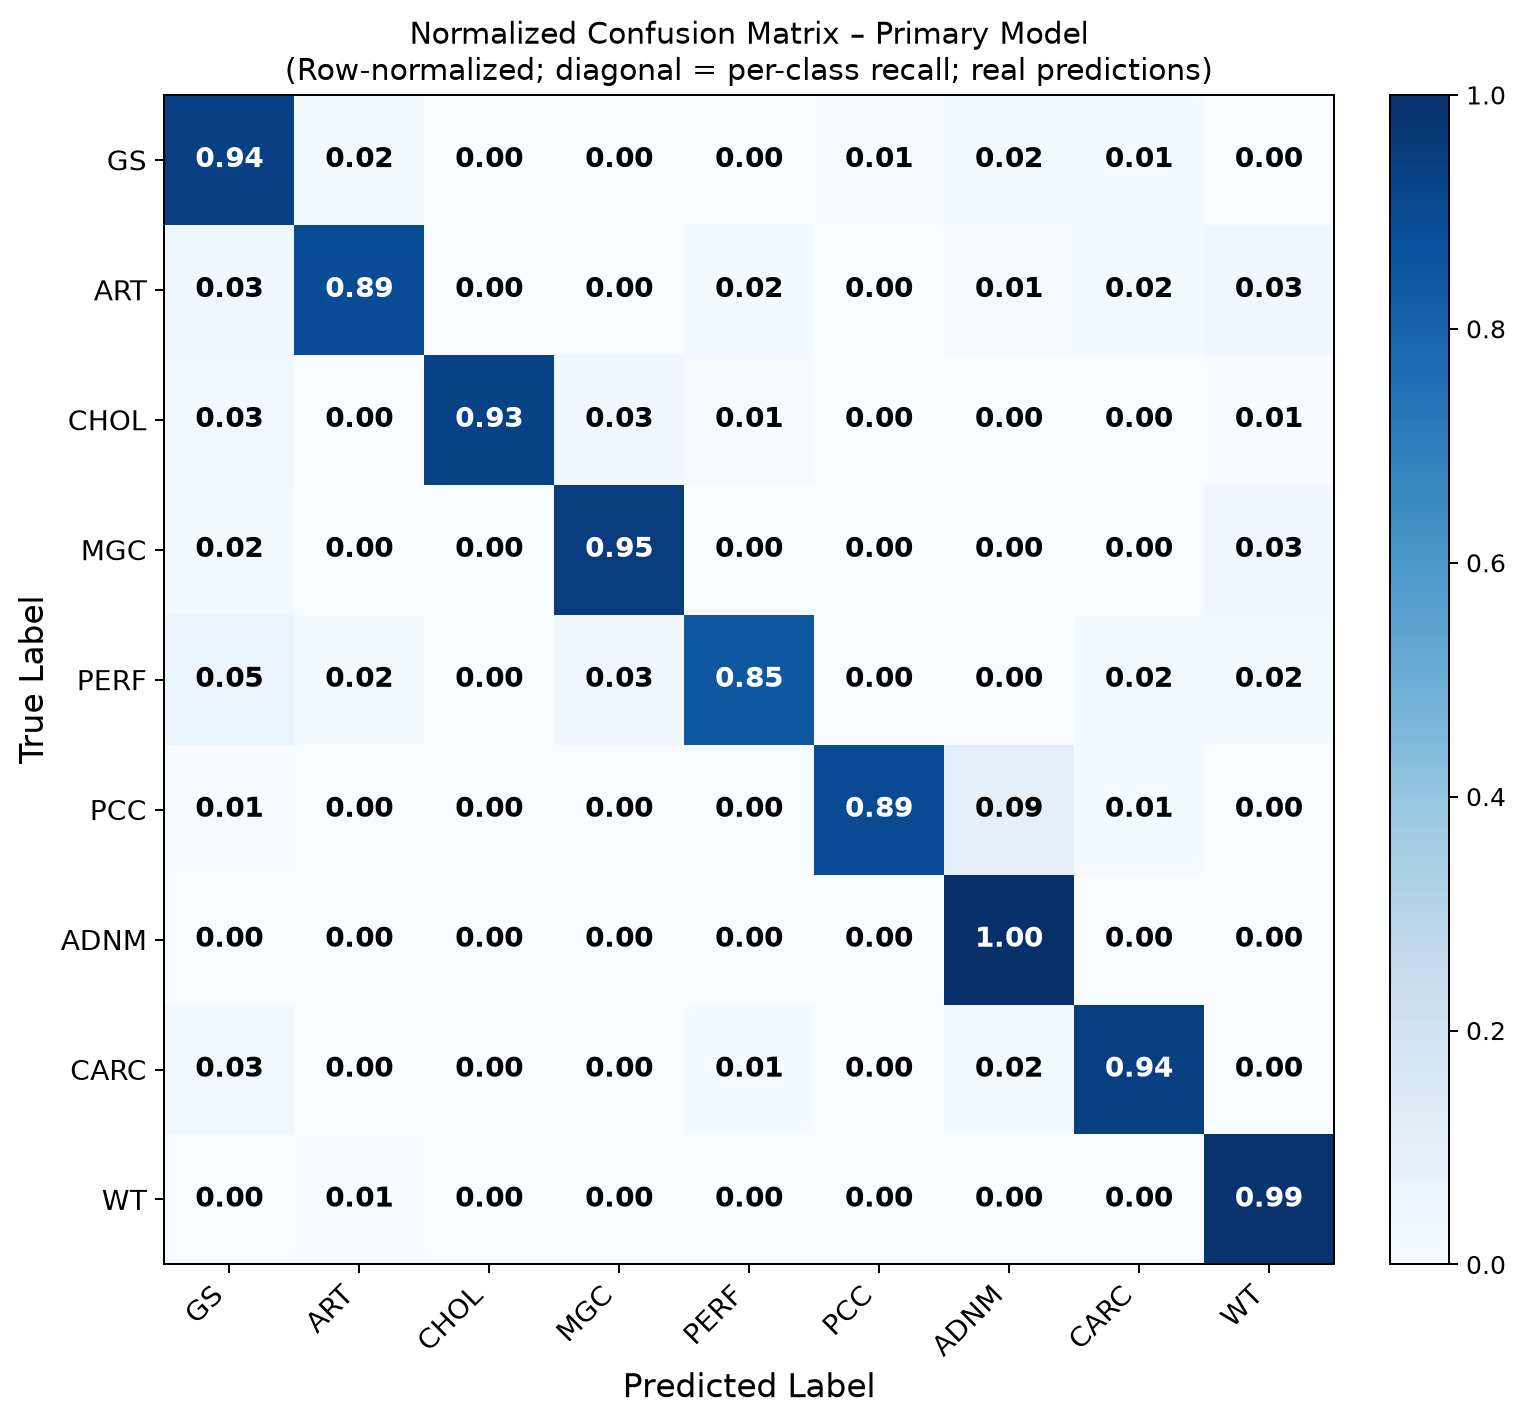
\includegraphics[width=0.42\textwidth]{figures/confusion_normalized}\hfill
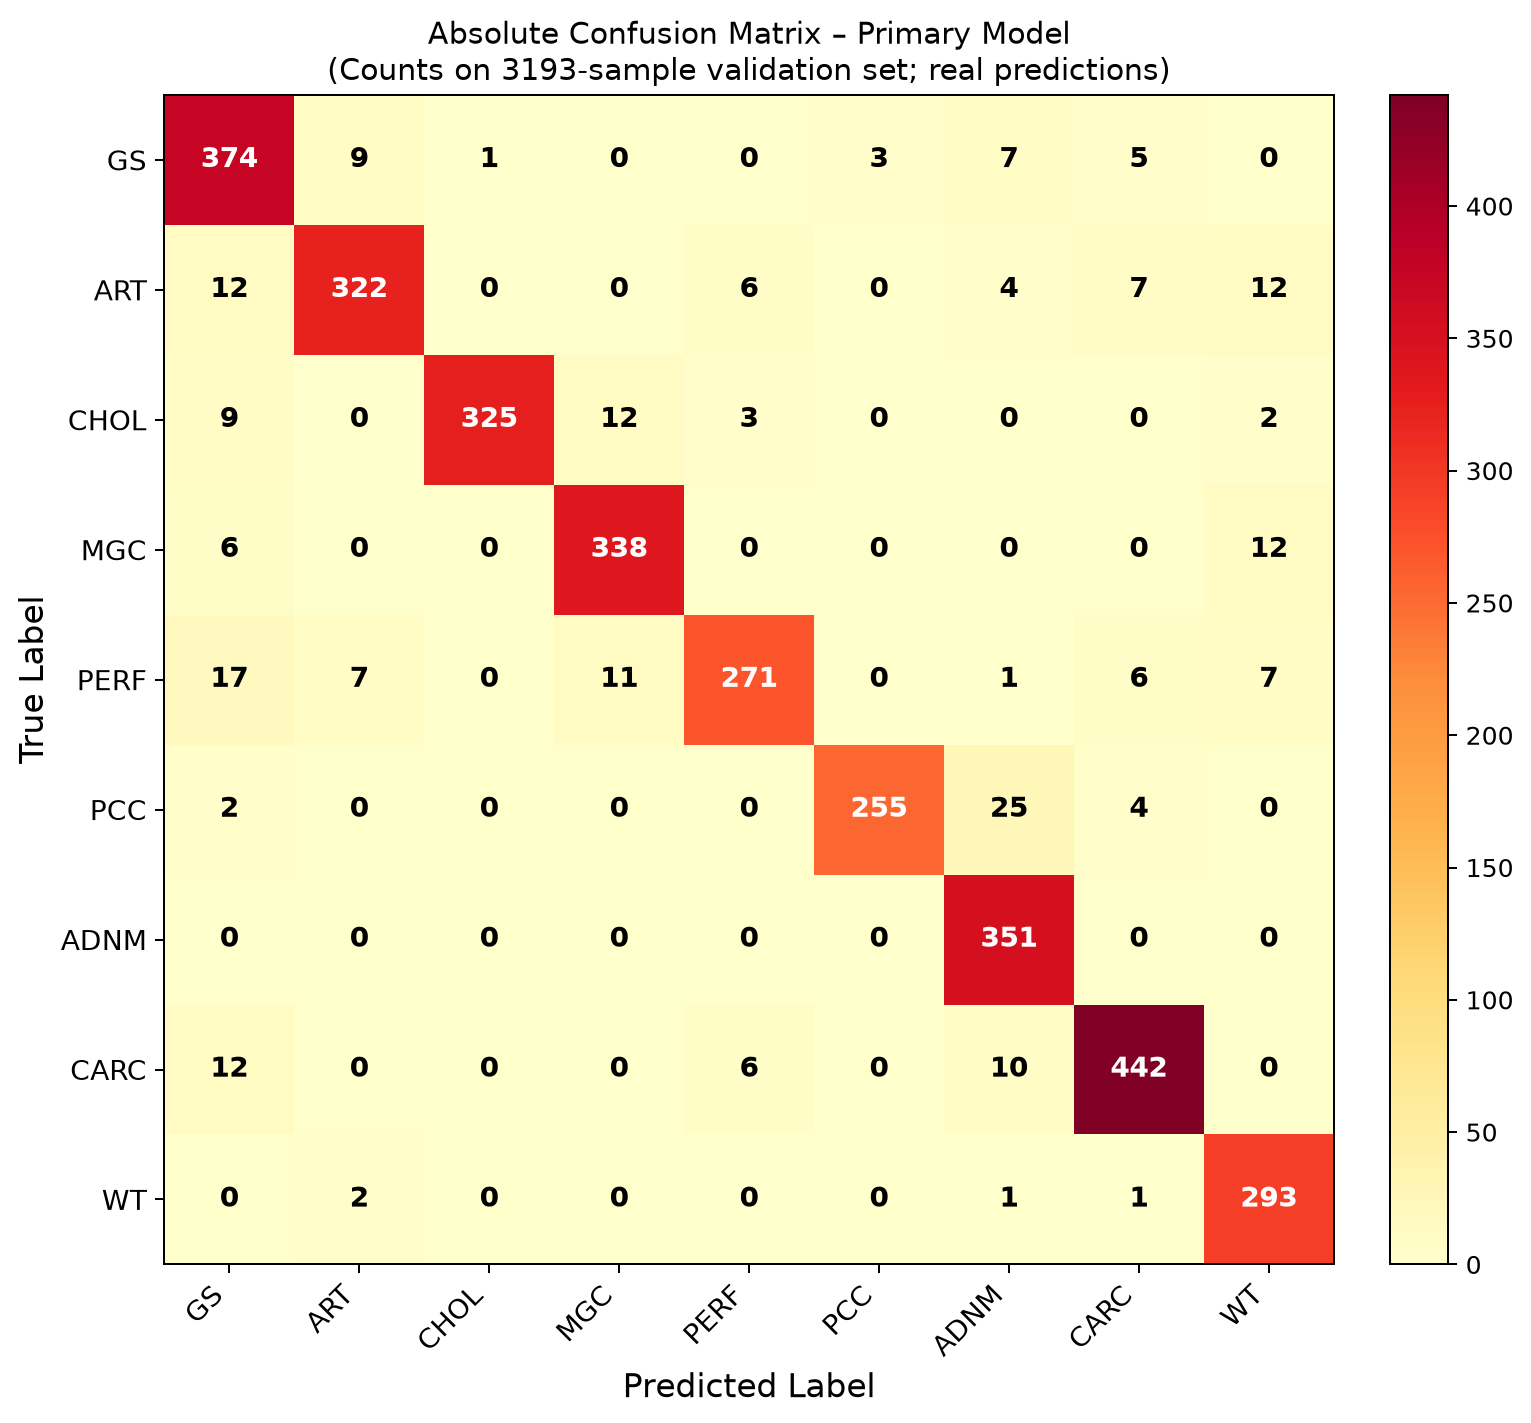
\includegraphics[width=0.42\textwidth]{figures/confusion_absolute}
\caption{(a)~Normalised confusion matrix. Row-normalised values show per-class recall. The largest single confusion is Polyps \& Cholesterol Crystals~$\rightarrow$~Adenomyomatosis. (b)~Absolute confusion matrix. Raw sample counts on the 3,193-image corrected validation set.}
\label{fig:4a}
\end{figure*}

\begin{figure*}[!ht]
\centering
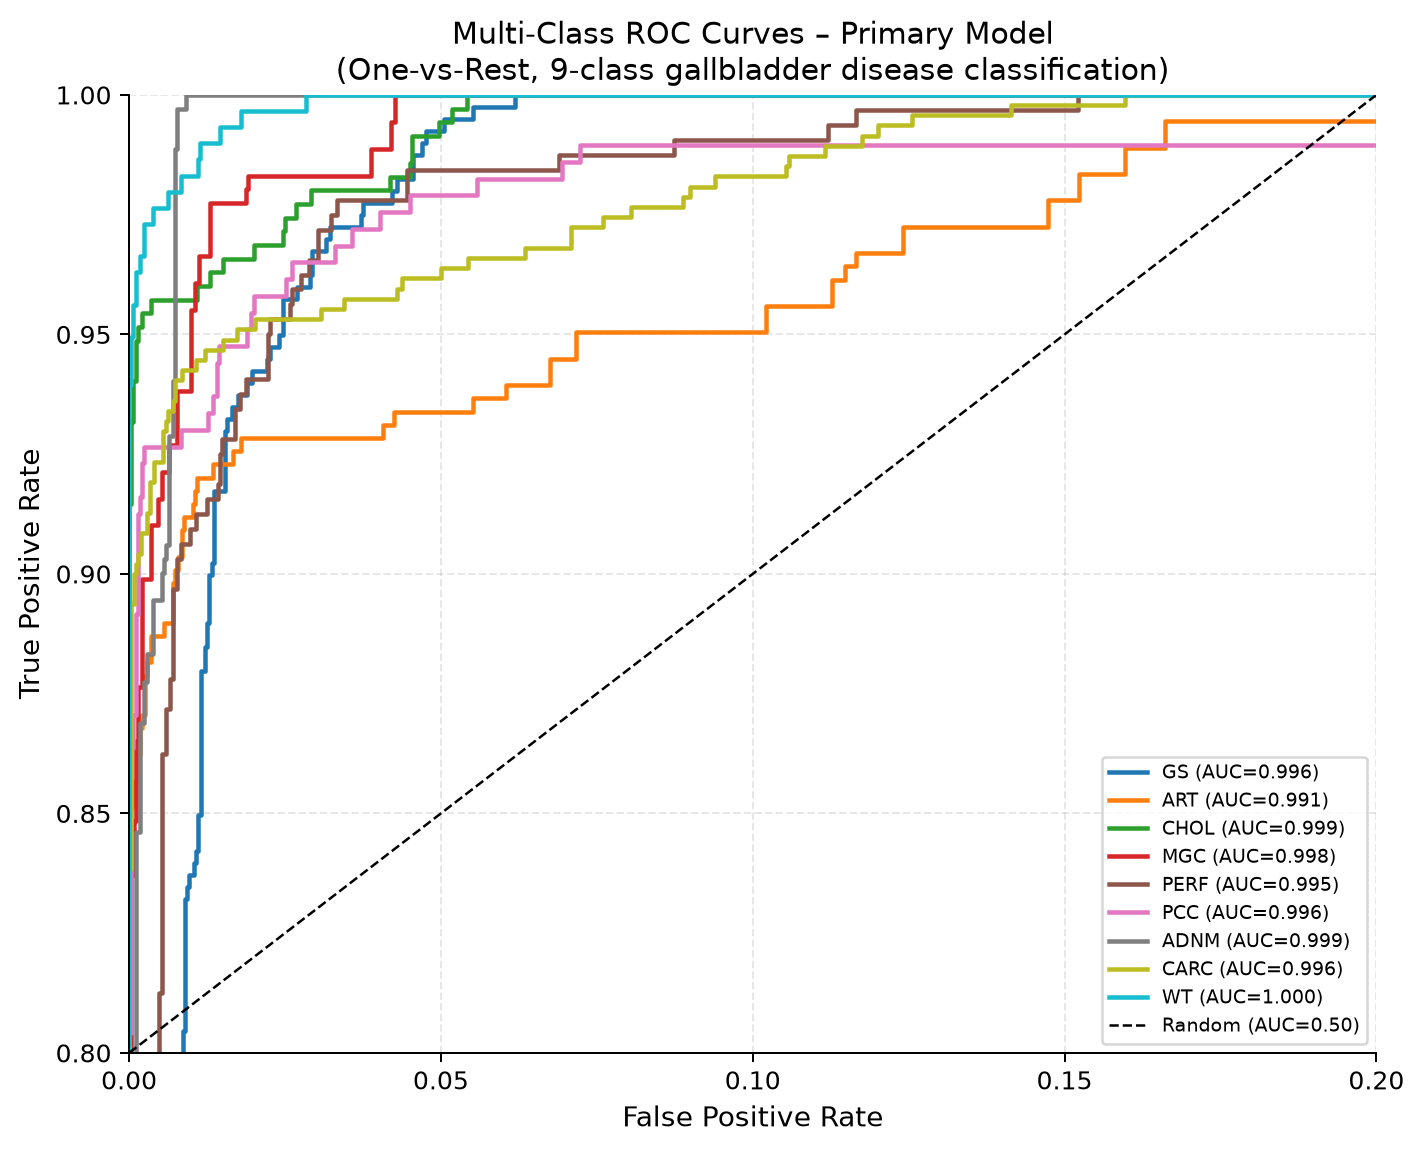
\includegraphics[width=0.6\textwidth]{figures/roc_curves.png}
\caption{One-vs-rest ROC curves for all nine classes. Macro AUC~=~0.9965. Wall Thickening and Adenomyomatosis achieve AUC~$>$~0.999; Abdomen \& Retroperitoneum is lowest at 0.9911, still far above chance.}
\label{fig:5}
\end{figure*}

\subsection{Failure-case analysis}

Of the 3,193 corrected validation images, the model misclassifies 222 (6.95\%), and eight confusion pairs together account for just over half of all errors (113 of 222, 50.9\%): Polyps~\&~Cholesterol Crystals~$\rightarrow$~Adenomyomatosis (25 images), Perforation~$\rightarrow$~Gallstones (17), Abdomen~\&~Retroperitoneum~$\rightarrow$~Gallstones (12), Abdomen~\&~Retroperitoneum~$\rightarrow$~Wall Thickening (12), Cholecystitis~$\rightarrow$~Membranous/Gangrenous Cholecystitis (12), Membranous/Gangrenous Cholecystitis~$\rightarrow$~Wall Thickening (12), Carcinoma~$\rightarrow$~Gallstones (12), and Perforation~$\rightarrow$~Membranous/Gangrenous Cholecystitis (11). Three patterns stand out. The single largest error, Polyps~\&~Cholesterol Crystals~$\rightarrow$~Adenomyomatosis (25 cases), links two benign, morphologically similar entities that both present as echogenic mural foci on ultrasound. Perforation, meanwhile, is confused with Gallstones (17 cases, its single largest error source) and with Membranous/Gangrenous Cholecystitis (11), together accounting for 28 of its total errors, consistent with perforation radiologically overlapping both stone disease and severe gangrenous wall change. A third pattern, Cholecystitis~$\rightarrow$~Membranous/Gangrenous Cholecystitis (12) and Membranous/Gangrenous Cholecystitis~$\rightarrow$~Wall Thickening (12), forms a severity-spectrum confusion chain, the clinically least dangerous direction among the top pairs since all three classes prompt continued attention. Carcinoma~$\rightarrow$~Gallstones (12) is more consequential by contrast: a missed-malignancy error read as benign.

To ground this in specific examples, Fig.~\ref{fig:6} shows two high-confidence wrong predictions from the two weakest classes. A true-Perforation image is classified Gallstones with 99.6\% confidence (the same pattern noted above); its Grad-CAM++ heatmap concentrates on a bright, shadow-adjacent structure, a reasonable-looking but wrong diagnostic cue. A true-Gallstones image is classified Abdomen~\&~Retroperitoneum with 93.6\% confidence, an error direction outside the top eight pairs above. In both cases the model is highly confident despite being wrong, and the heatmap looks anatomically plausible rather than obviously off-target, so heatmap plausibility alone would not have flagged either error. That is a real limitation of plausibility as an error-detection signal on its own (Section~\ref{sec:discussion}.2).

\begin{figure*}[!ht]
\centering
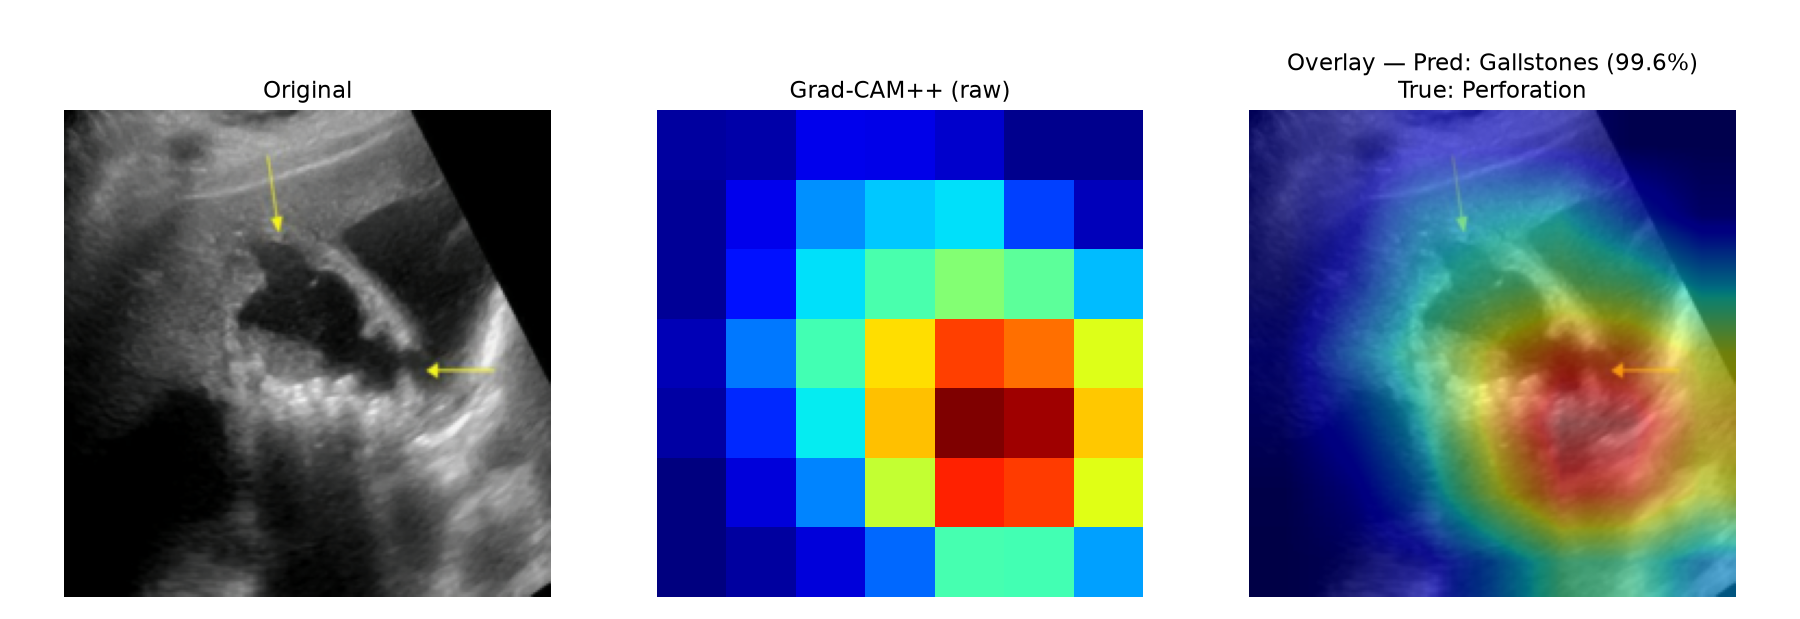
\includegraphics[width=0.42\textwidth]{figures/failure_case_perforation}\hfill
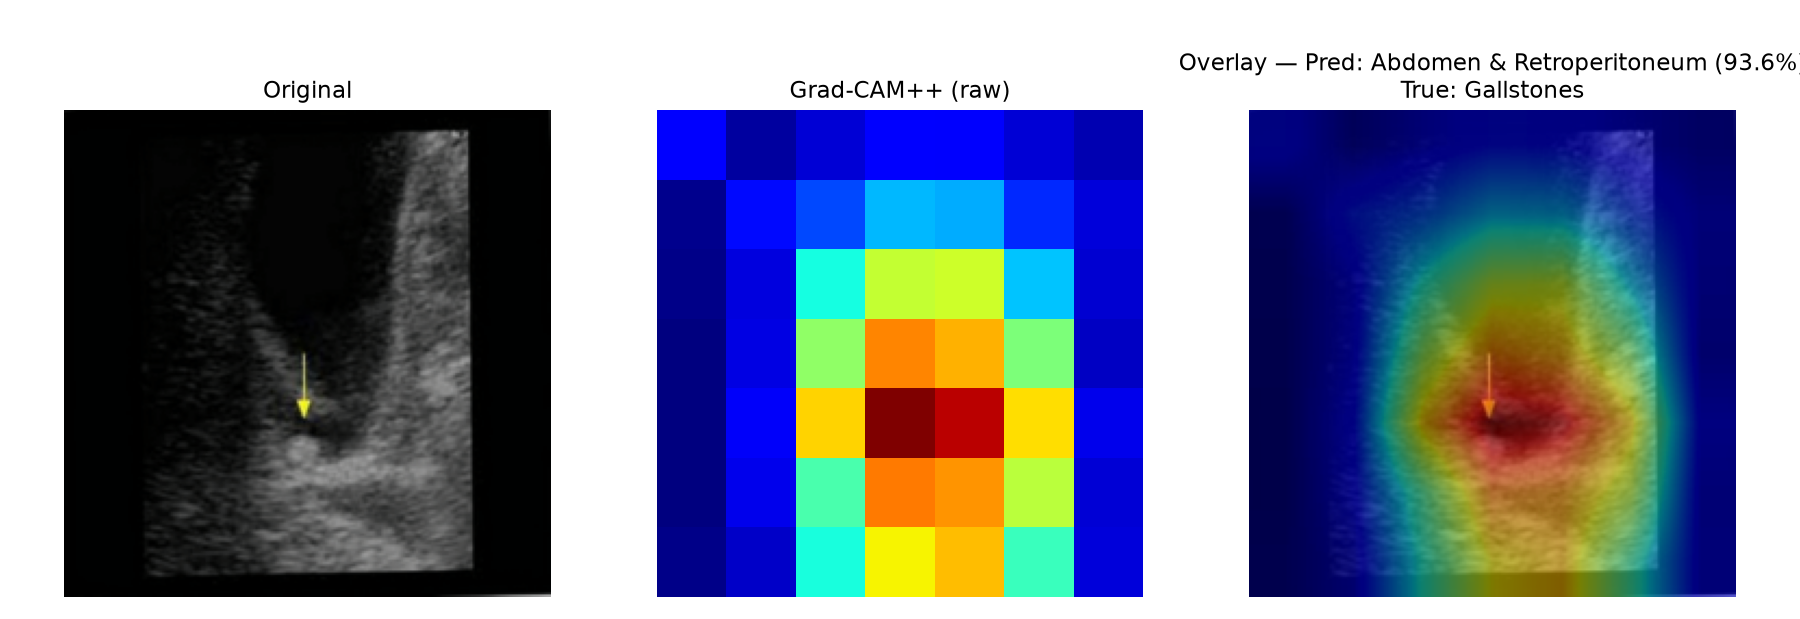
\includegraphics[width=0.42\textwidth]{figures/failure_case_gallstones}
\caption{Two representative high-confidence misclassifications, one from each of the two weakest classes (Table~\ref{tbl:4}). Left: true Perforation predicted Gallstones (99.6\%) --- the single largest confusion-pair direction for Perforation (Pattern~2). Right: true Gallstones predicted Abdomen~\&~Retroperitoneum (93.6\%). Each panel shows the original ultrasound, the Grad-CAM++ heatmap, and the overlay. Both heatmaps are anatomically plausible-looking despite the wrong label, illustrating that heatmap plausibility alone does not reliably flag classification errors.}
\label{fig:6}
\end{figure*}

\textbf{Confidence and calibration signal (uncalibrated).} Mean softmax confidence is 0.974 on correctly classified images but 0.771 on misclassified ones, suggesting a confidence-threshold triage could surface many mistakes for review. This is only a raw-softmax observation, though, and raw softmax confidence is known to be an unreliable proxy for true probability \cite{ref42}; the miscalibration it points to is quantified and formally corrected (ECE, Brier score, temperature scaling) in Section~\ref{sec:results}.4.

\subsection{Qualitative and quantitative comparison of XAI methods}

All five XAI methods are applied to the primary model across all nine disease classes. \textbf{Grad-CAM} produces smooth, region-level heatmaps, while \textbf{Grad-CAM++} consistently generates sharper, more focused activation patches, particularly for Carcinoma and Membranous/Gangrenous Cholecystitis, where the discriminative feature is a localised wall irregularity rather than a diffuse region. \textbf{Saliency Maps} highlight fine-grained pixel-level evidence but carry more background noise, and \textbf{Eigen-CAM}, being class-agnostic, highlights the single dominant activation pattern regardless of predicted class, which makes it informative as a sanity baseline but weaker for per-class discrimination. \textbf{Score-CAM} produces heatmaps similar in character to Grad-CAM++, since both explicitly condition on the target class's evidence, one via second-order gradients and the other via masked-input forward passes.

\textit{XAI Finding (2):} Grad-CAM++ and Score-CAM produce noticeably sharper, more class-discriminative localization than Grad-CAM, Saliency, or Eigen-CAM for Carcinoma and Membranous/Gangrenous Cholecystitis, where the discriminative feature is a localised wall structure rather than a broad region. For Cholecystitis and Wall Thickening, all CAM-family methods produce similar heatmaps, consistent with those classes having larger, more uniformly distributed discriminative features.

\textit{XAI Finding (3):} In representative examples across all nine classes, the primary model's Grad-CAM++ attention appears anatomically plausible when inspected visually: acoustic shadow for Gallstones, focal wall attention for Carcinoma, diffuse wall-adjacent change for the mutually-confusable MGC/Perforation pair, small mural foci for the mutually-confusable Adenomyomatosis/PCC pair, and broader body-wide attention for ART and Wall Thickening. This is the authors' visual assessment, not a claim of anatomical correctness validated against clinician-defined regions of interest (Section~\ref{sec:limitations}).

Grad-CAM++ and Score-CAM improve most clearly over Grad-CAM for Carcinoma and Membranous/Gangrenous Cholecystitis, where the model needs to localise subtle wall changes rather than broad regions. Saliency Maps consistently highlight gallbladder boundary pixels, while Eigen-CAM's class-agnostic pattern is visibly less anatomically focused than the other four methods across every row. Supplementary Material A contains the full, non-cherry-picked per-class Grad-CAM++ gallery and a cross-method comparison grid showing all five XAI methods side by side for one representative image per class.

Figs.~\ref{fig:8} and \ref{fig:8b} show, respectively, ten and a further ten representative images spanning all nine classes (two to three per class, 20 in total), each with the original, raw Grad-CAM++ heatmap, overlay, and the model's predicted-class confidence, to confirm the heatmap patterns above are not an artefact of a single cherry-picked image per class. The remaining images of the full 54-image, non-cherry-picked gallery (six samples per class) are in Supplementary Material A.

\begin{figure*}[!ht]
\centering
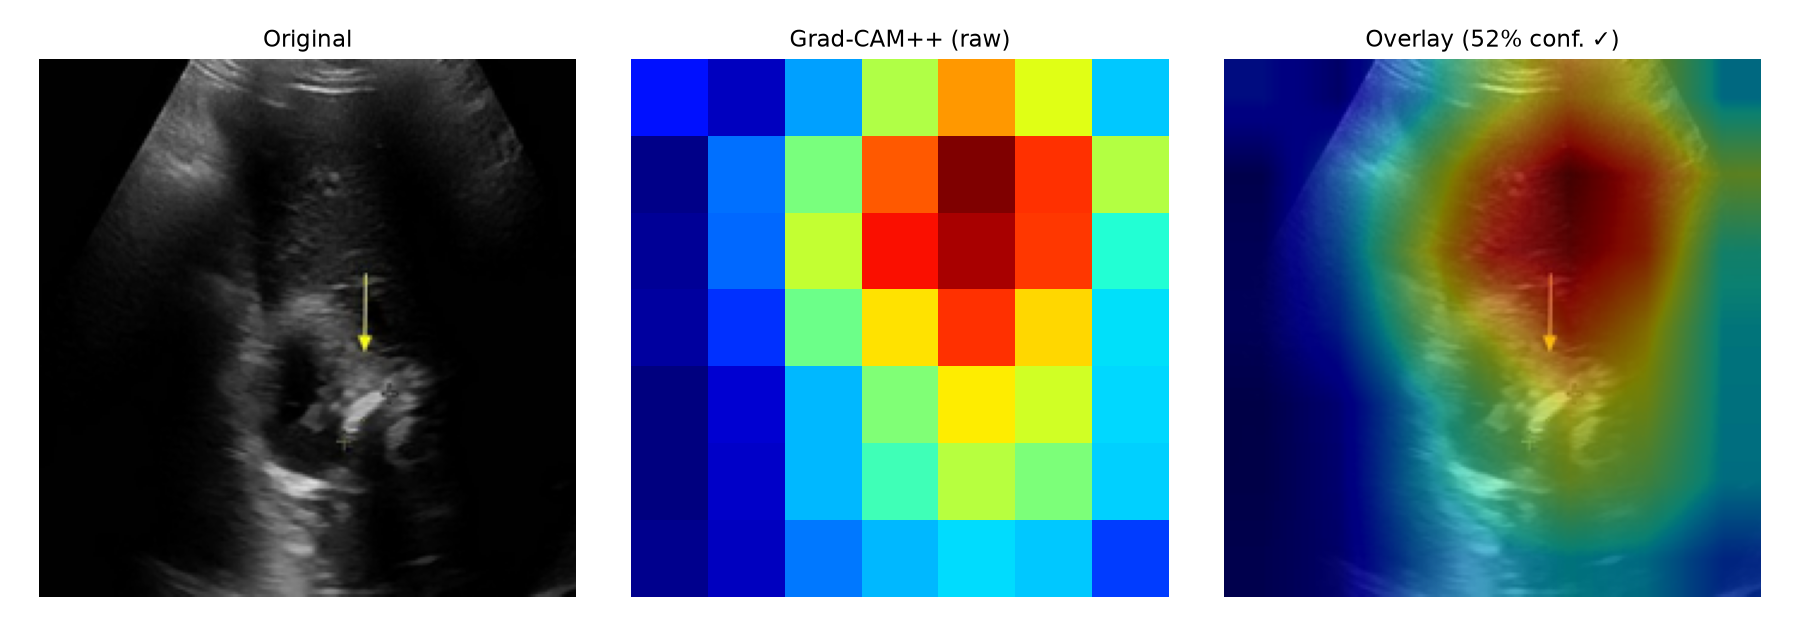
\includegraphics[width=0.48\linewidth]{figures/fig7_expanded/01_gallstones_01}\hfill
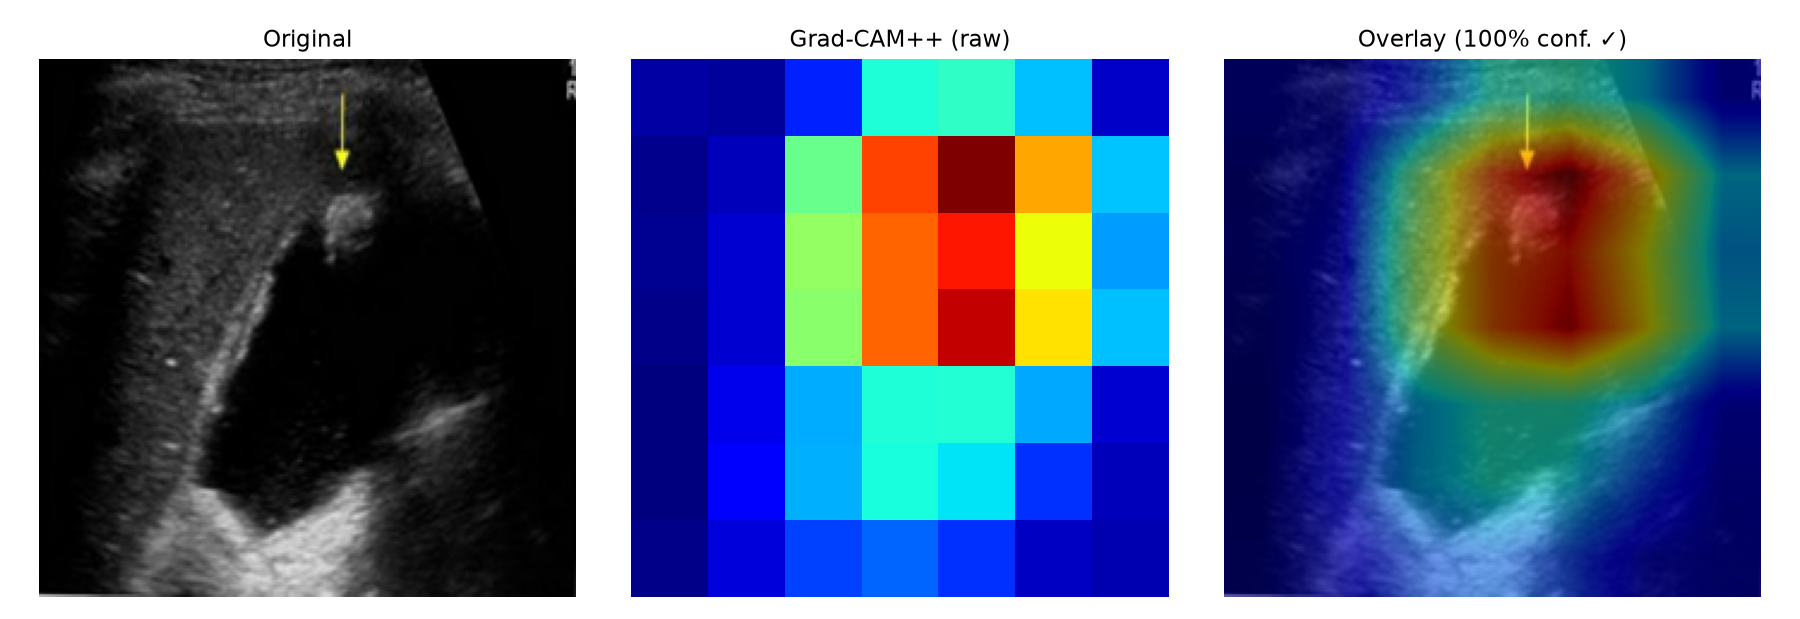
\includegraphics[width=0.48\linewidth]{figures/fig7_expanded/01_gallstones_02}\\[2pt]
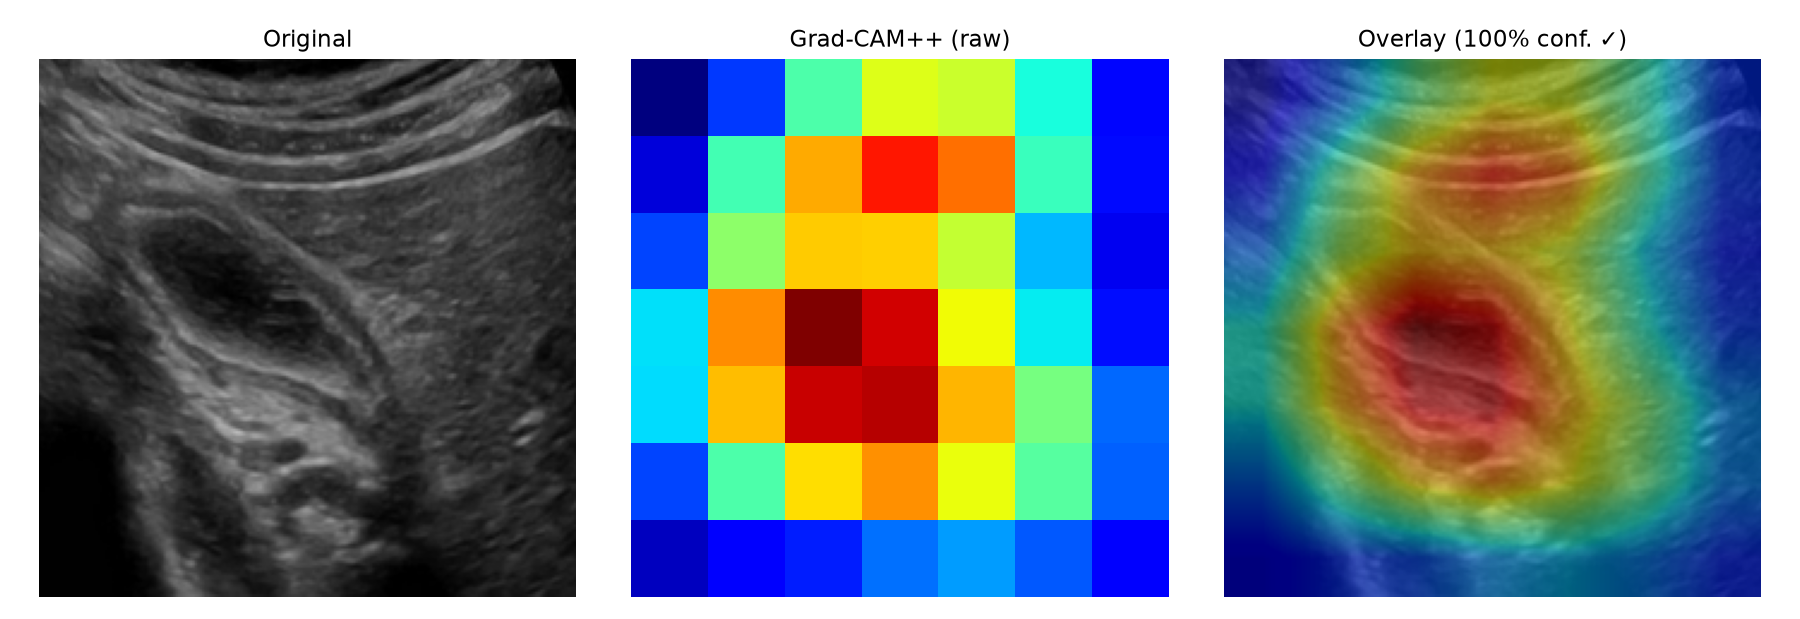
\includegraphics[width=0.48\linewidth]{figures/fig7_expanded/01_gallstones_03}\hfill
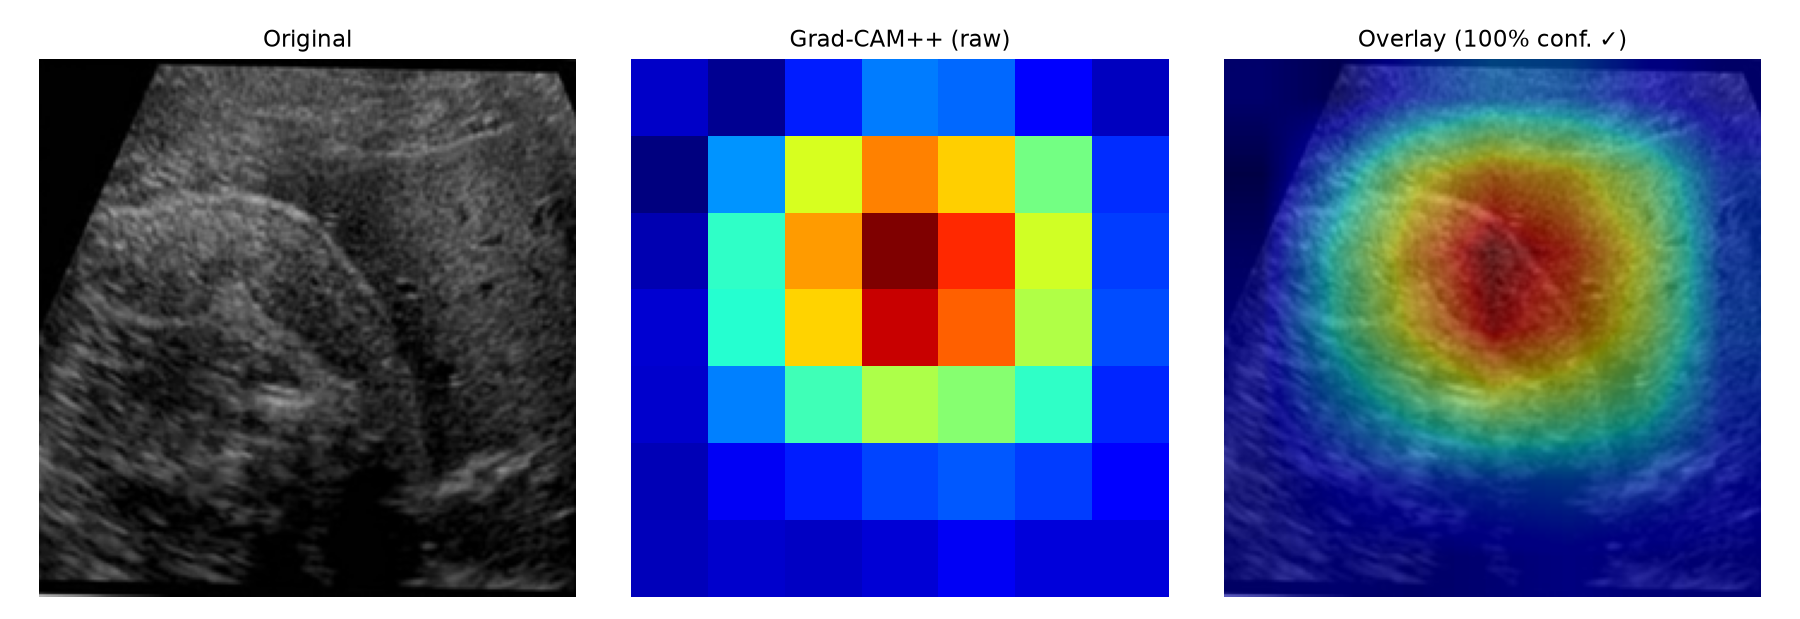
\includegraphics[width=0.48\linewidth]{figures/fig7_expanded/02_abdomen_and_retroperitoneum_01}\\[2pt]
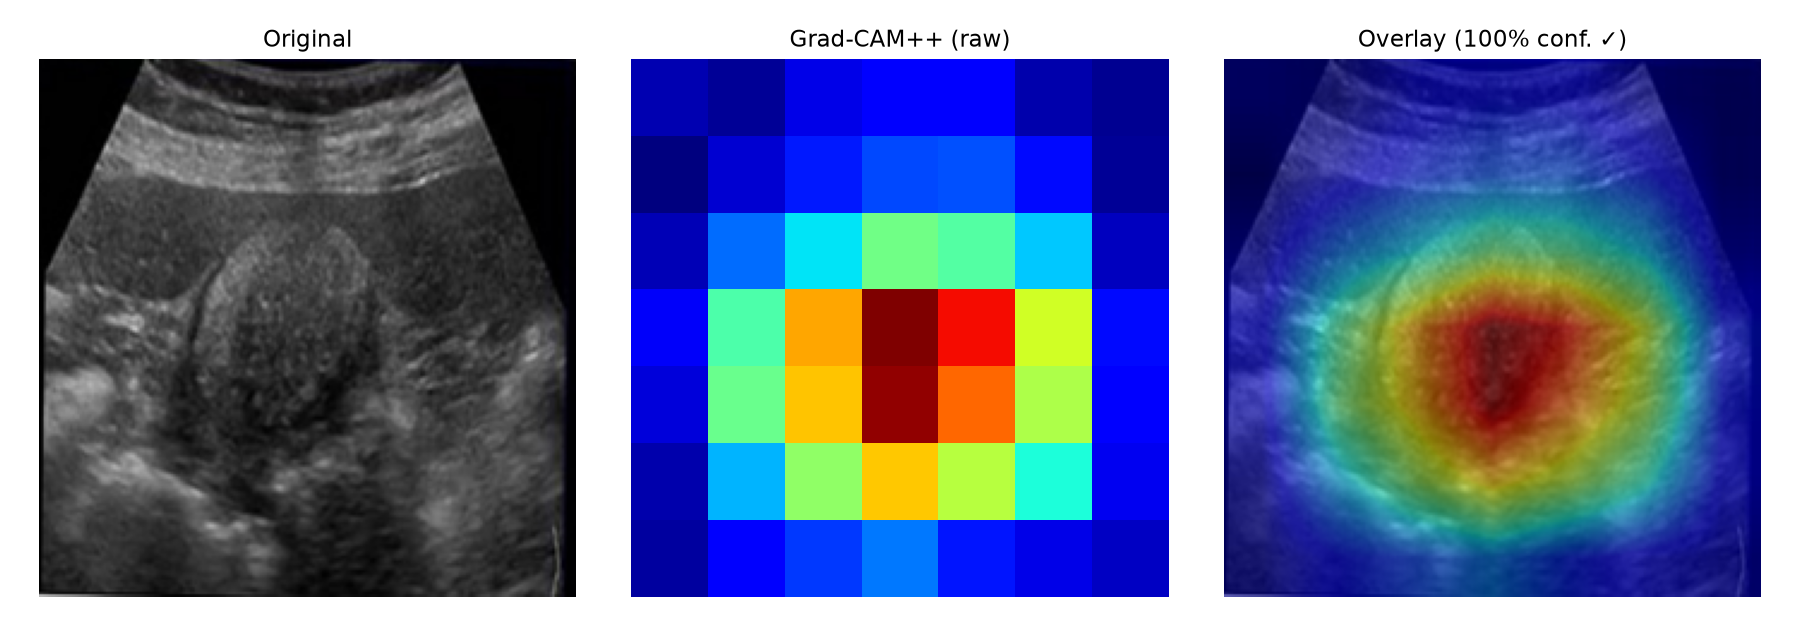
\includegraphics[width=0.48\linewidth]{figures/fig7_expanded/02_abdomen_and_retroperitoneum_02}\hfill
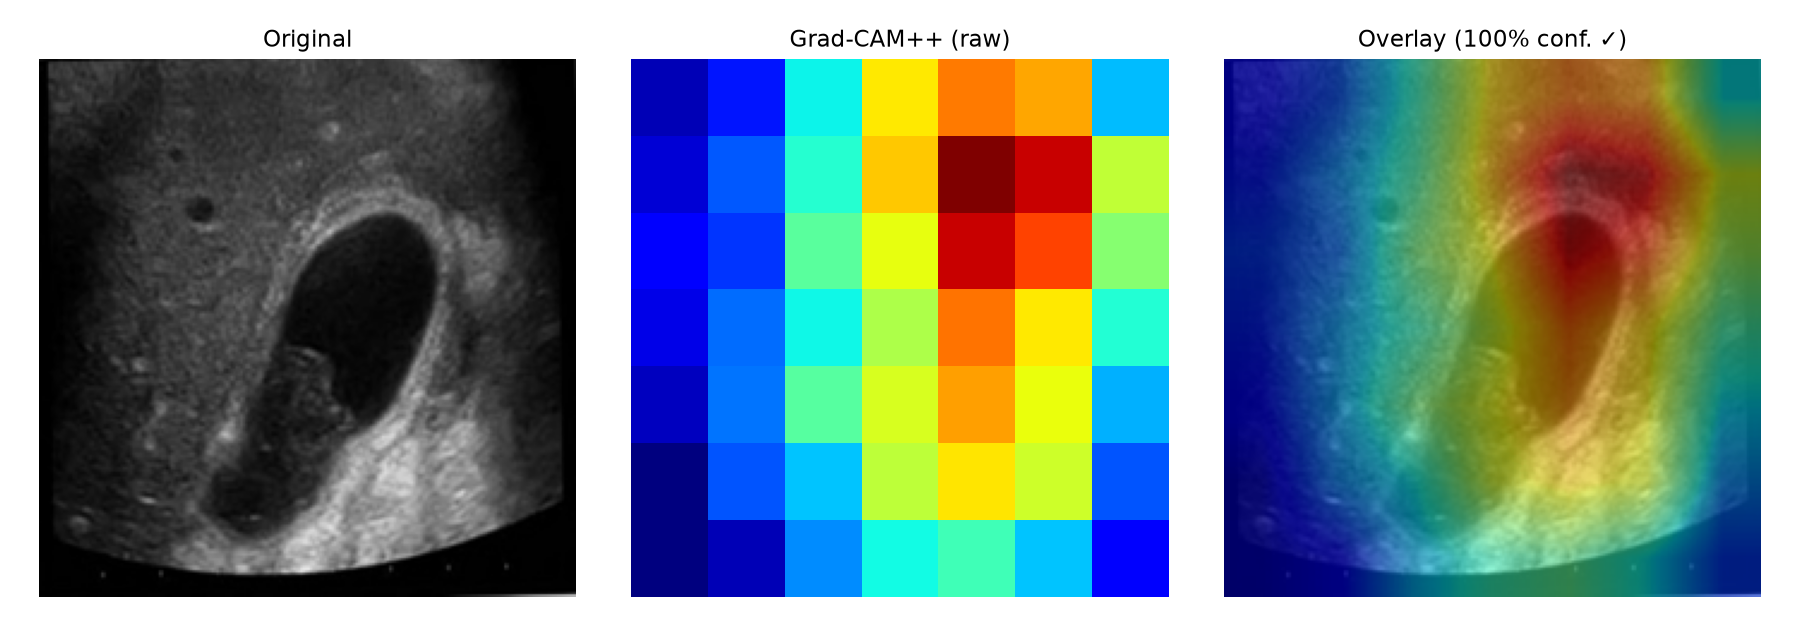
\includegraphics[width=0.48\linewidth]{figures/fig7_expanded/03_cholecystitis_01}\\[2pt]
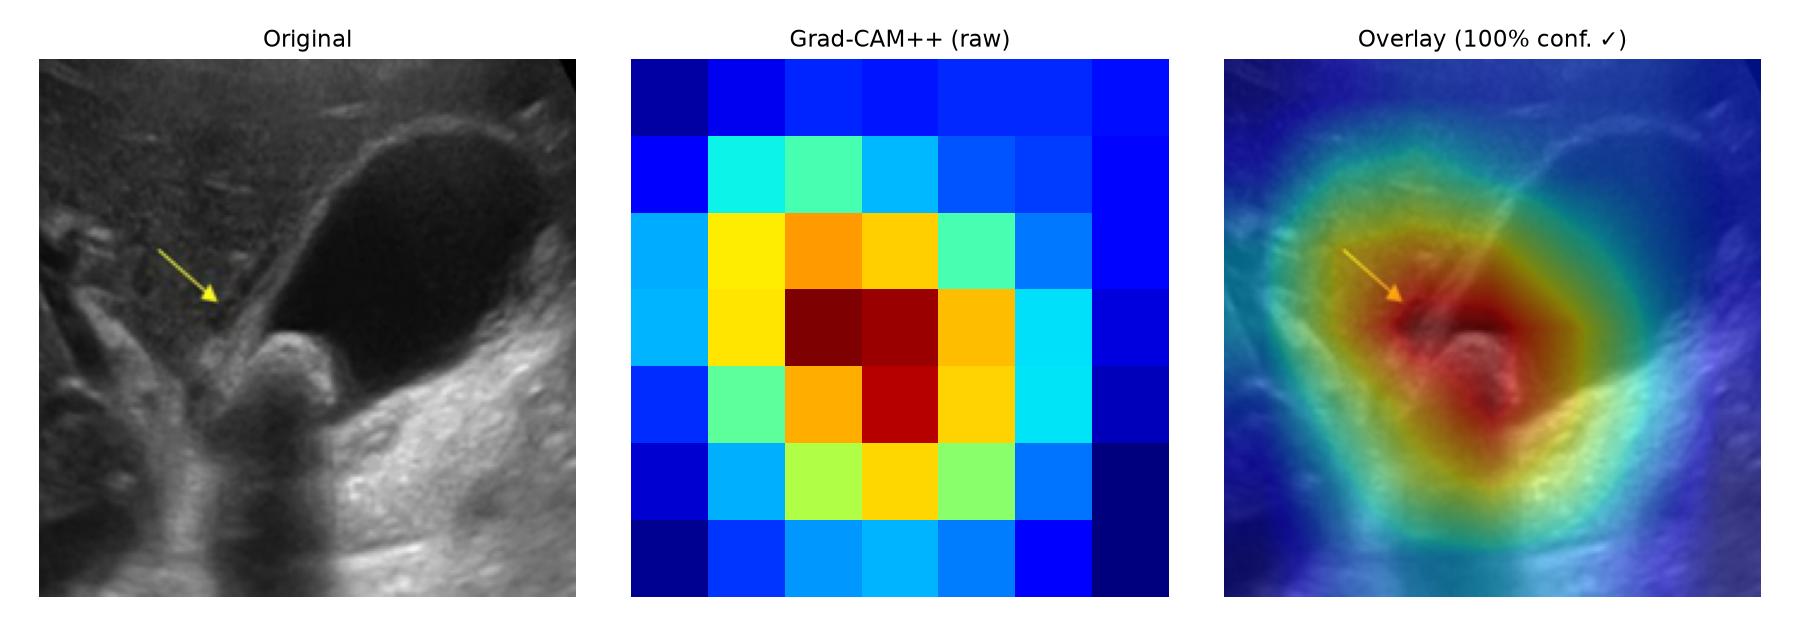
\includegraphics[width=0.48\linewidth]{figures/fig7_expanded/03_cholecystitis_02}\hfill
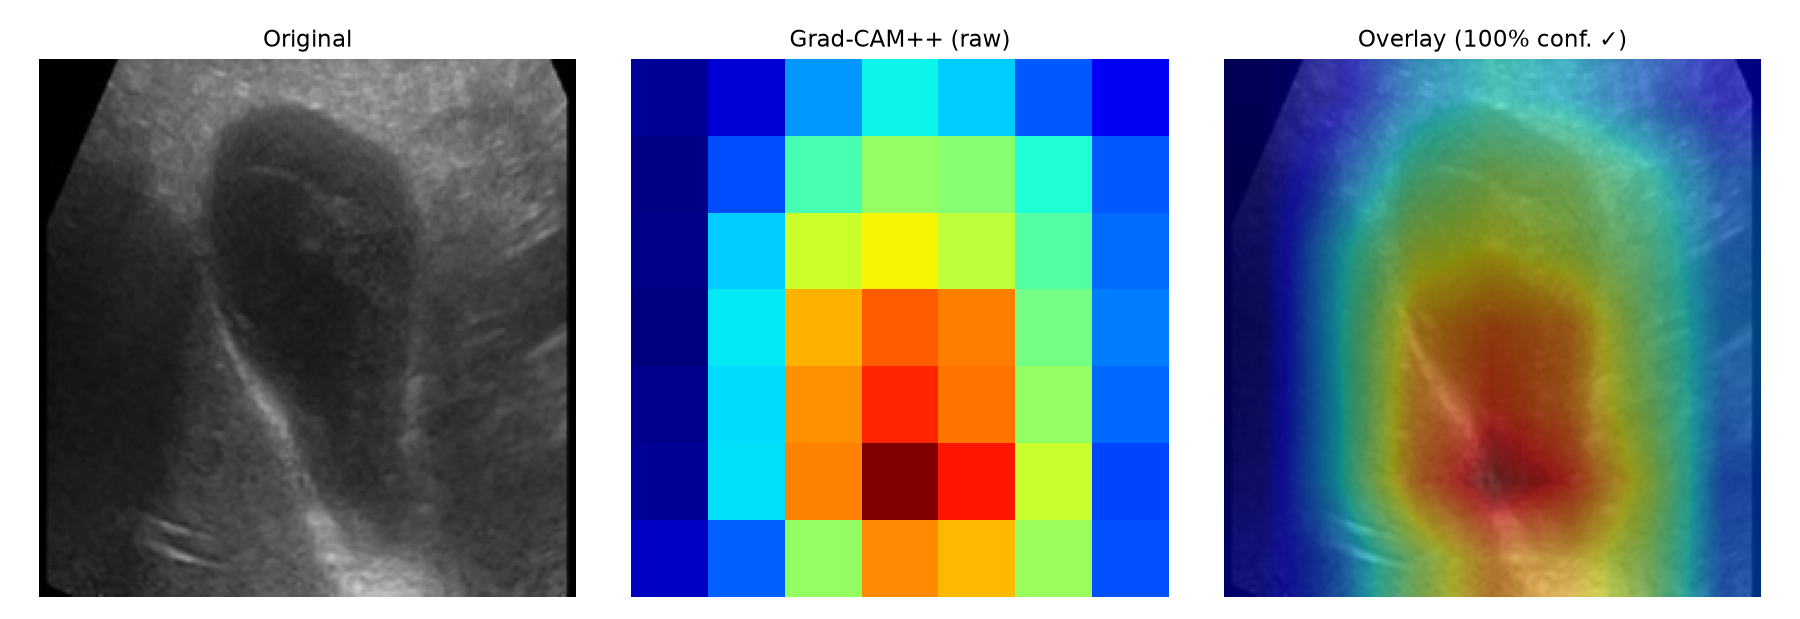
\includegraphics[width=0.48\linewidth]{figures/fig7_expanded/04_membranous_and_gangrenous_cholecystitis_01}\\[2pt]
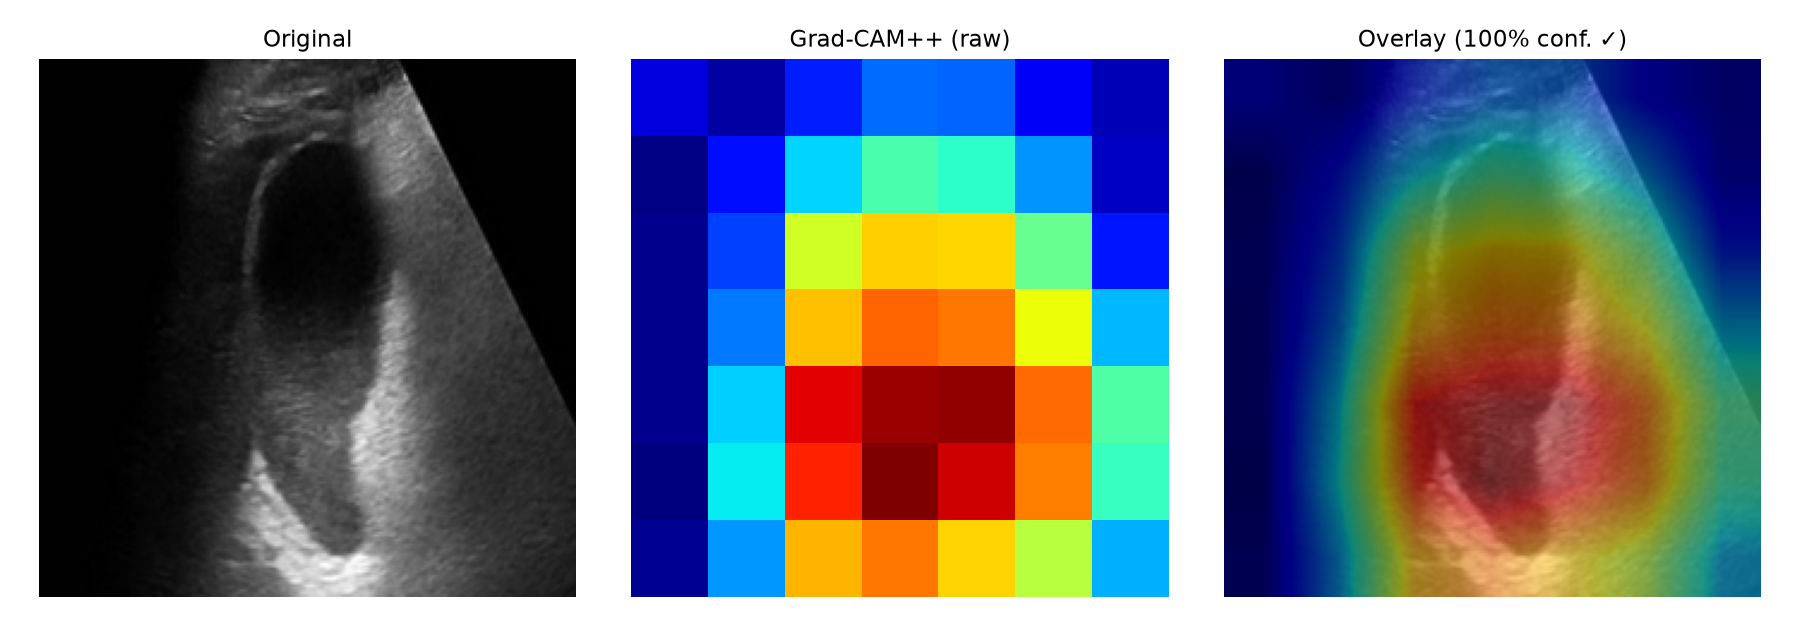
\includegraphics[width=0.48\linewidth]{figures/fig7_expanded/04_membranous_and_gangrenous_cholecystitis_02}\hfill
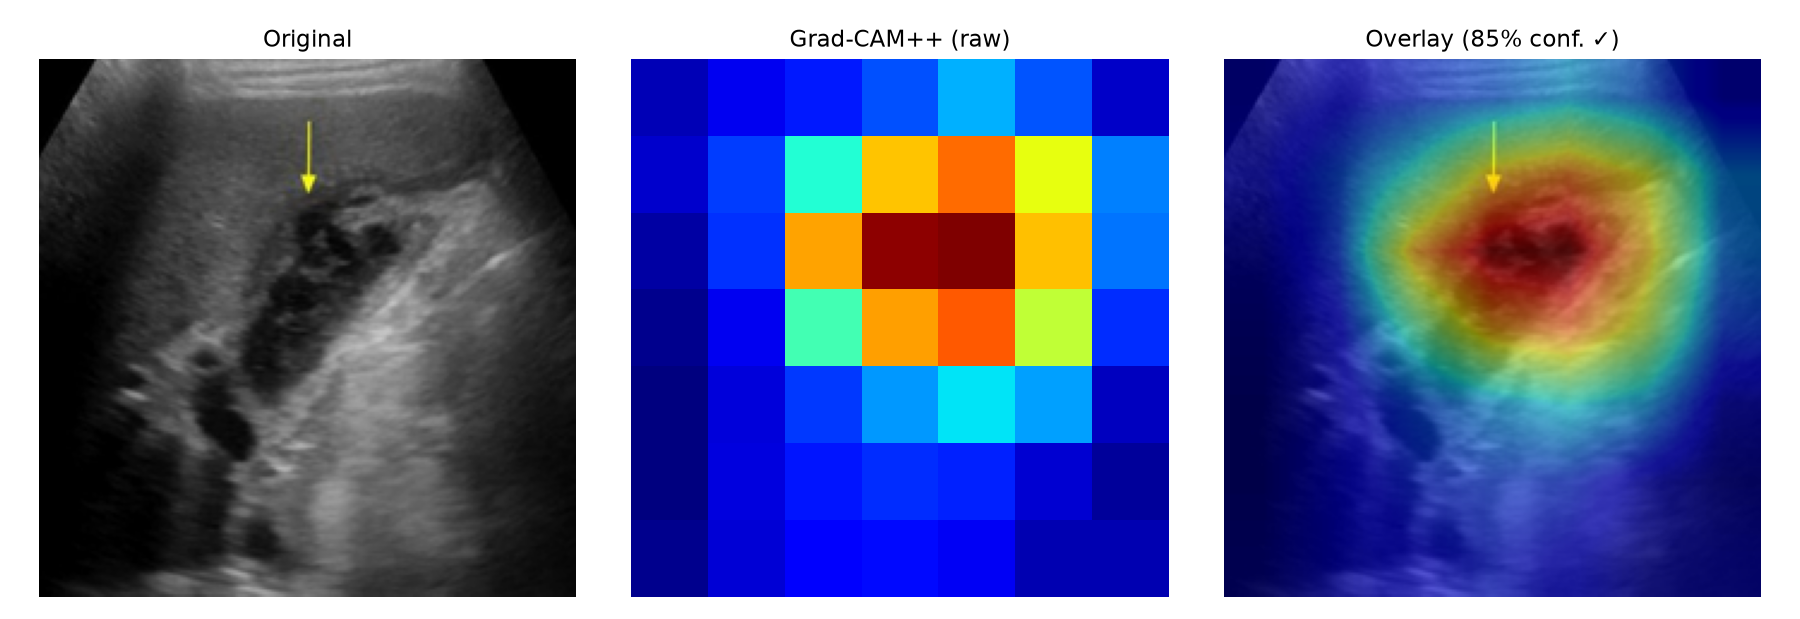
\includegraphics[width=0.48\linewidth]{figures/fig7_expanded/05_perforation_01}
\caption{Original image, raw Grad-CAM++ heatmap, and overlay for two-to-three representative images each of Gallstones, Abdomen \& Retroperitoneum, Cholecystitis, and Membranous/Gangrenous Cholecystitis, plus one of Perforation (continued in Fig.~\ref{fig:8b}). Each overlay panel is labelled with the model's predicted-class confidence and a \checkmark/\ding{55} marker for correctness. Attention concentrates on central image content in the region conventionally associated with the gallbladder wall and lumen, consistent with the class-specific patterns described in Section~\ref{sec:results}.3; this is a visual, non-clinician-validated observation (Section~\ref{sec:limitations}).}
\label{fig:8}
\end{figure*}

\begin{figure*}[!ht]
\centering
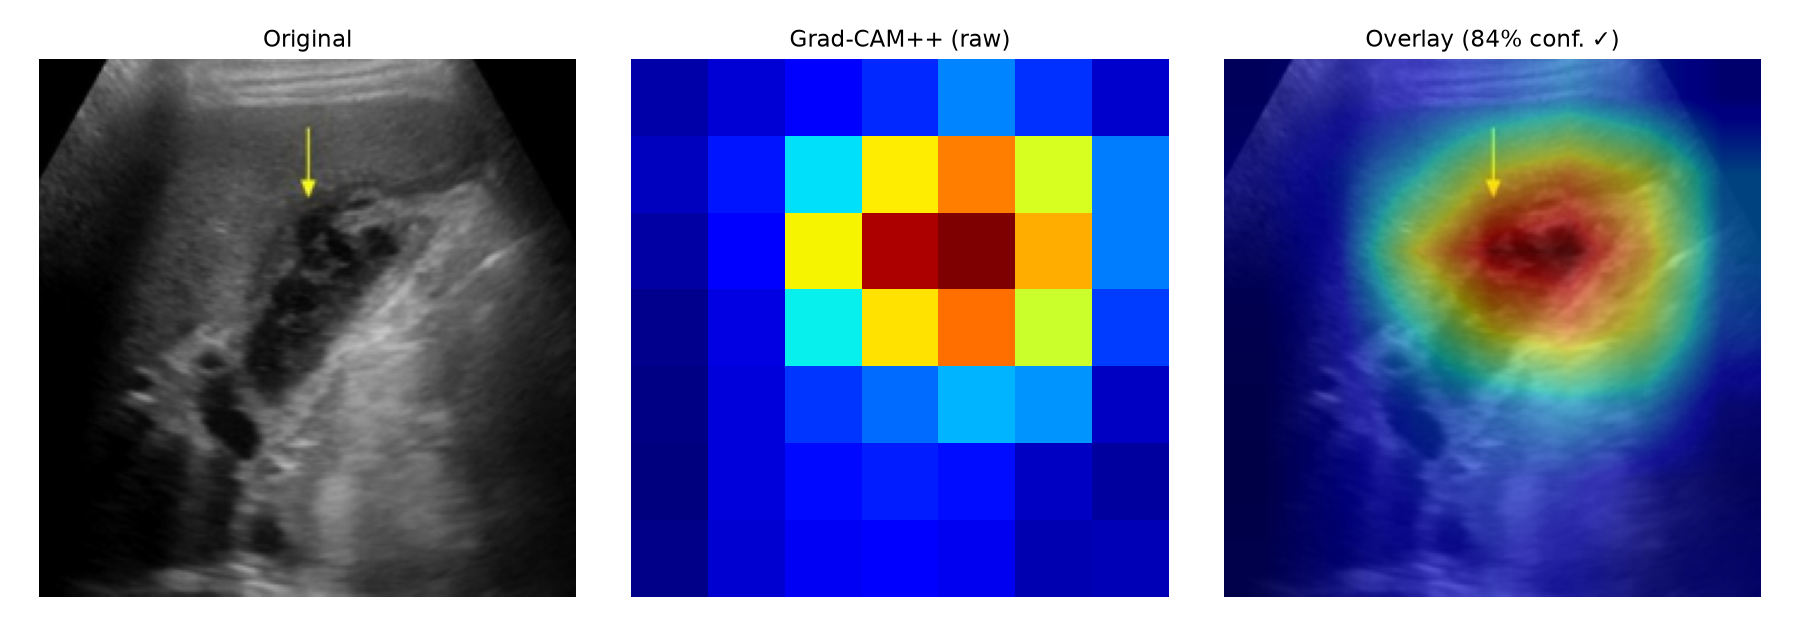
\includegraphics[width=0.48\linewidth]{figures/fig7_expanded/05_perforation_02}\hfill
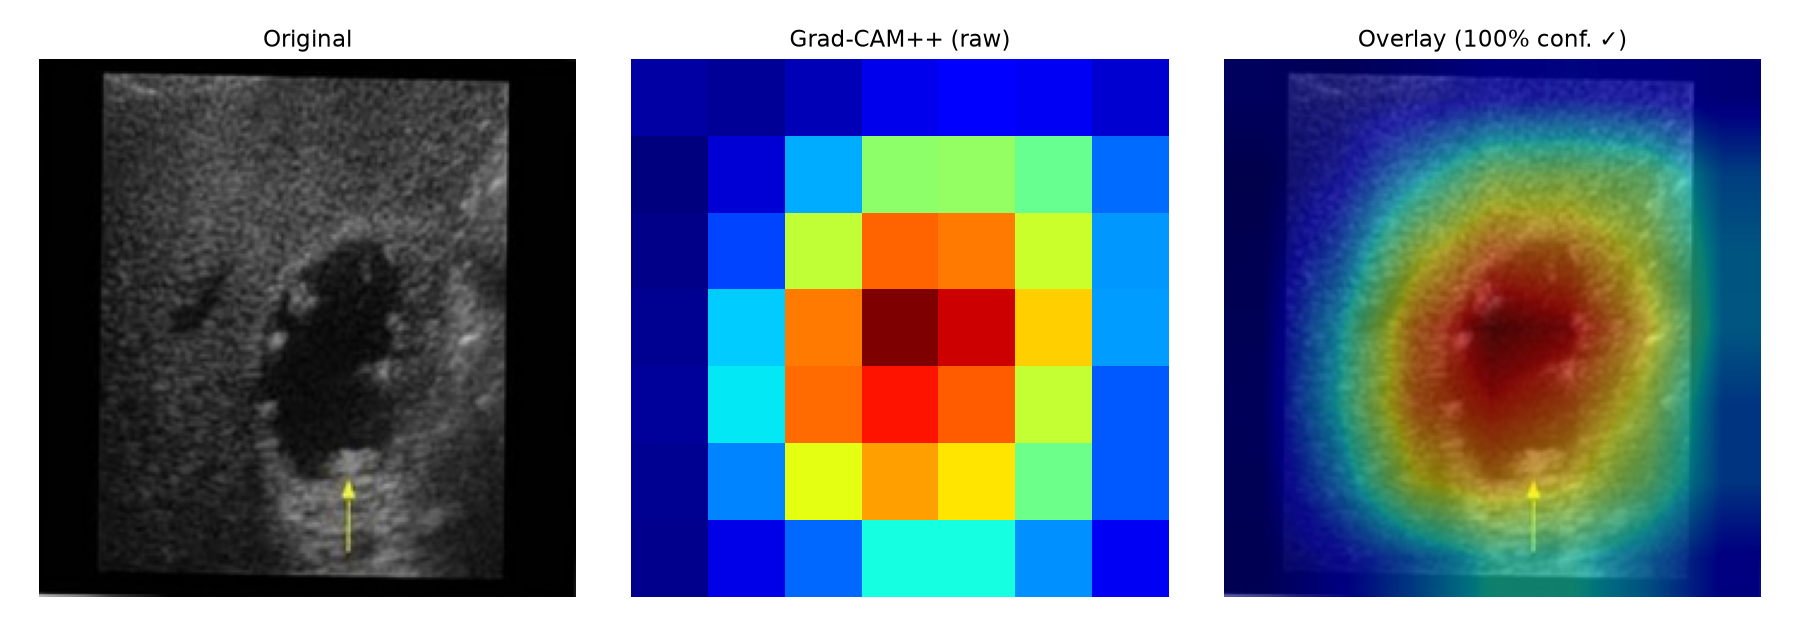
\includegraphics[width=0.48\linewidth]{figures/fig7_expanded/06_polyps_and_cholesterol_crystals_01}\\[2pt]
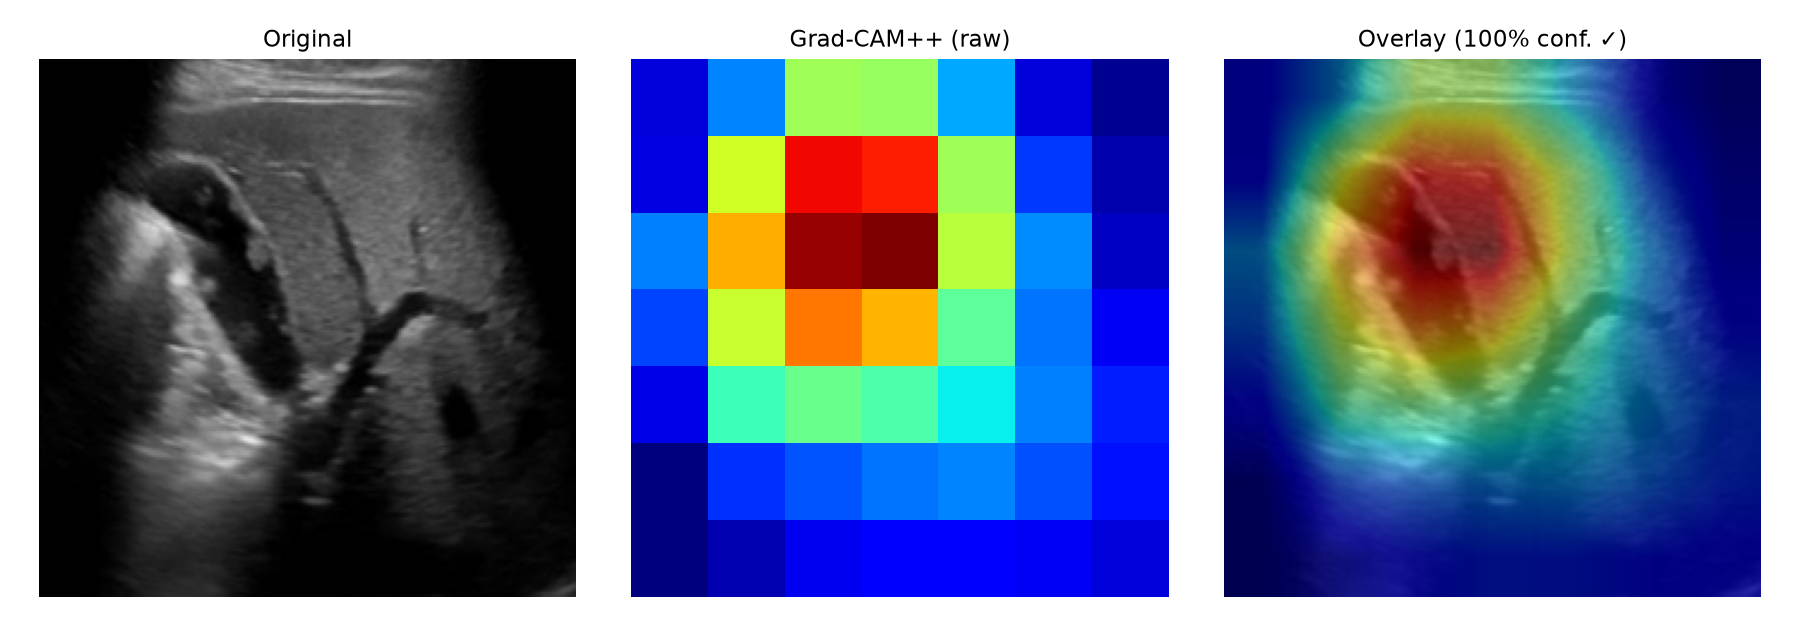
\includegraphics[width=0.48\linewidth]{figures/fig7_expanded/06_polyps_and_cholesterol_crystals_02}\hfill
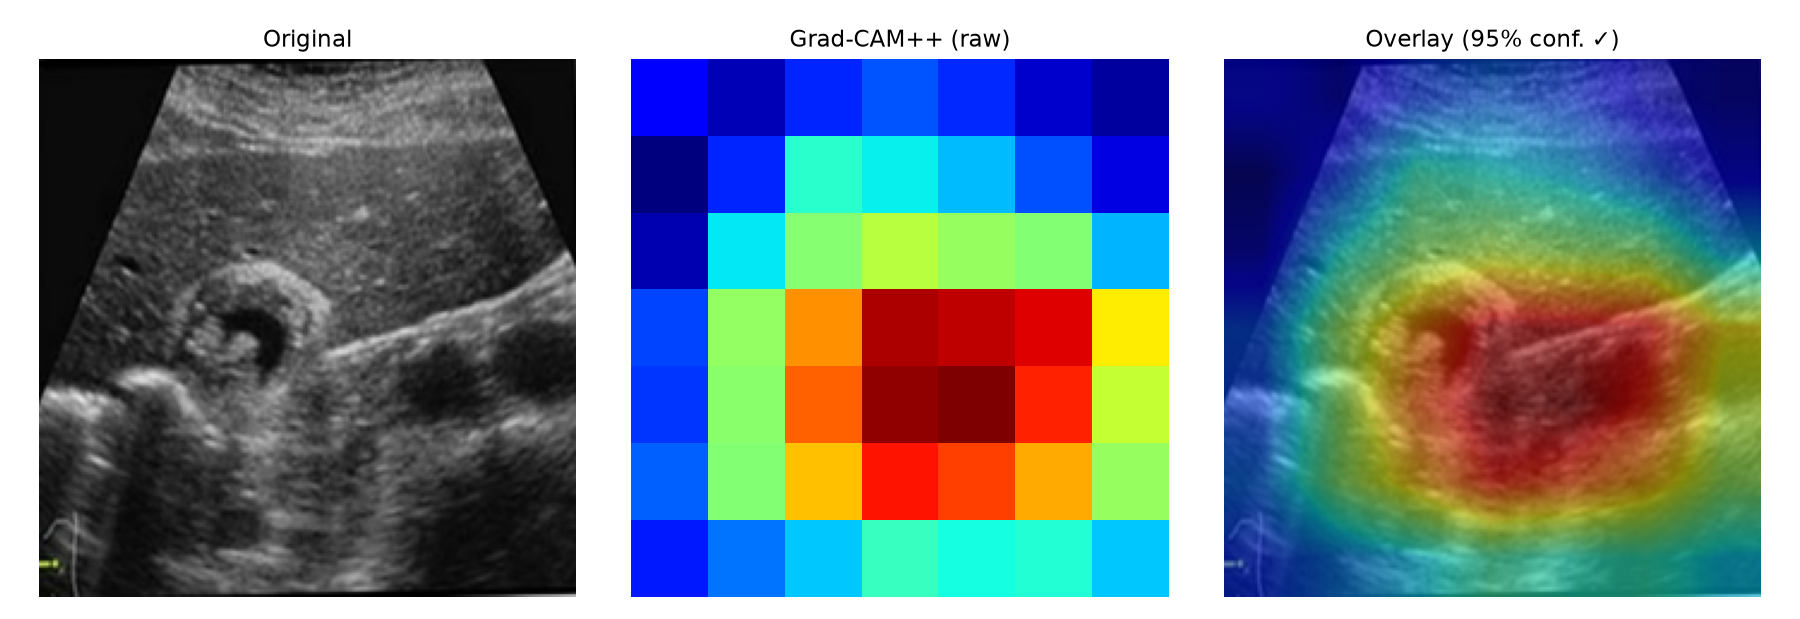
\includegraphics[width=0.48\linewidth]{figures/fig7_expanded/07_adenomyomatosis_01}\\[2pt]
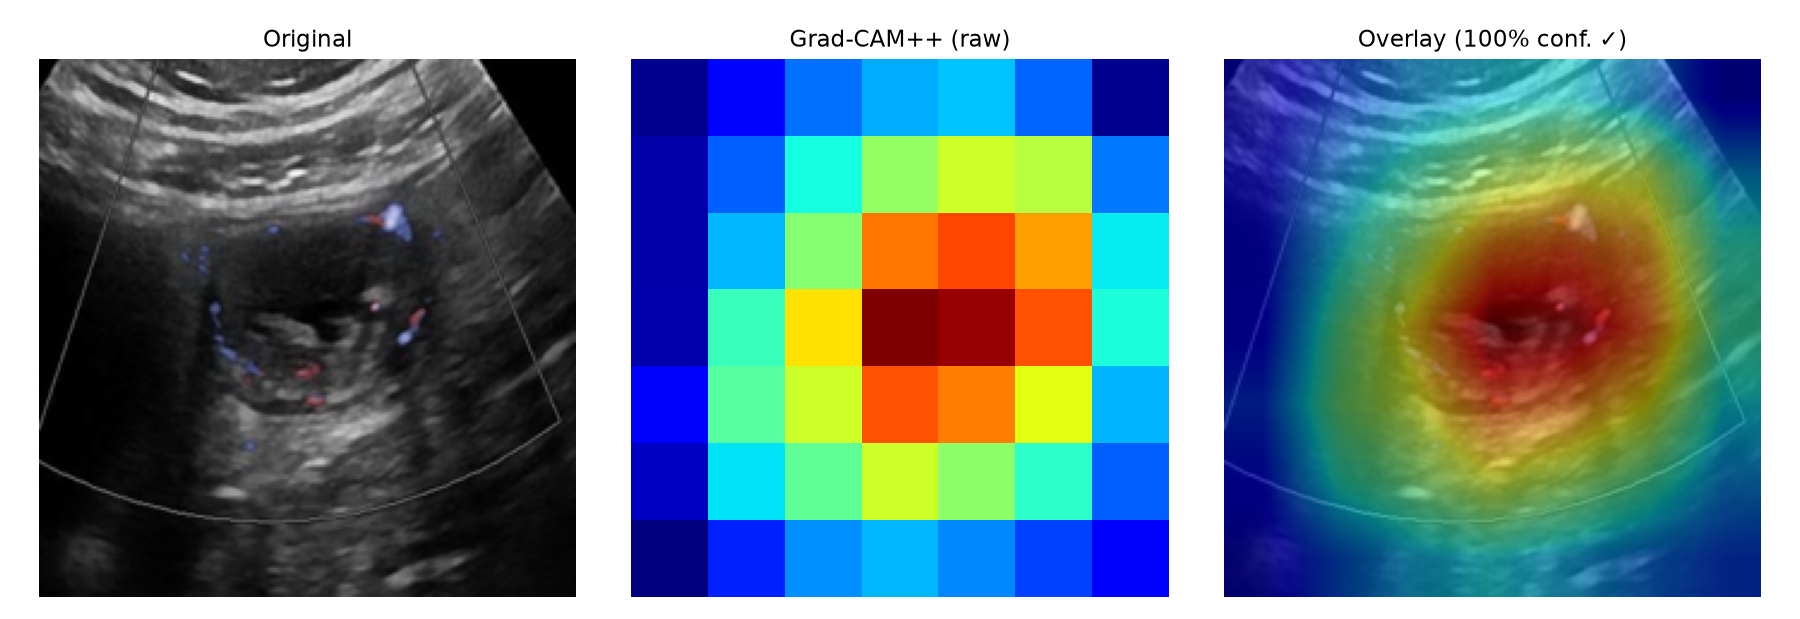
\includegraphics[width=0.48\linewidth]{figures/fig7_expanded/07_adenomyomatosis_02}\hfill
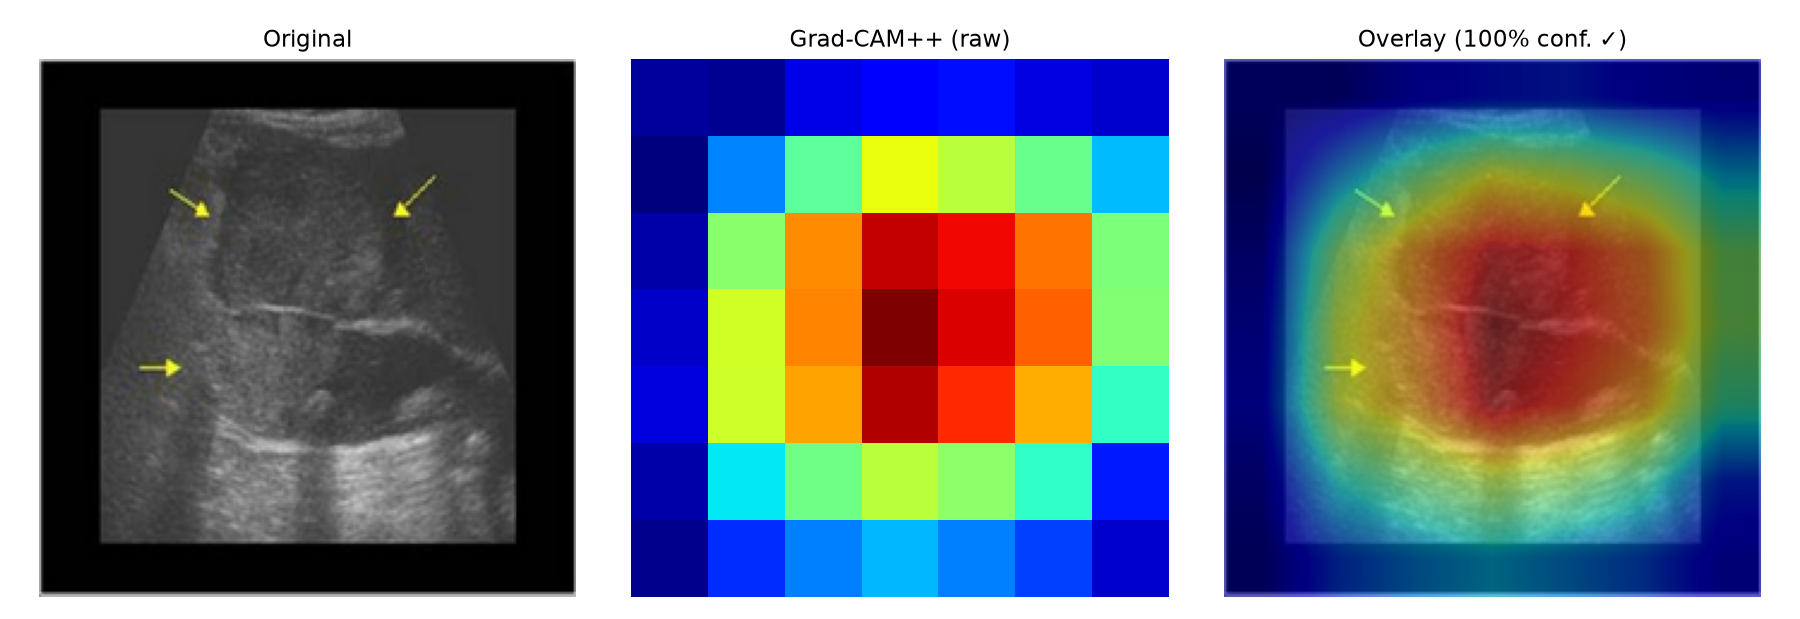
\includegraphics[width=0.48\linewidth]{figures/fig7_expanded/08_carcinoma_01}\\[2pt]
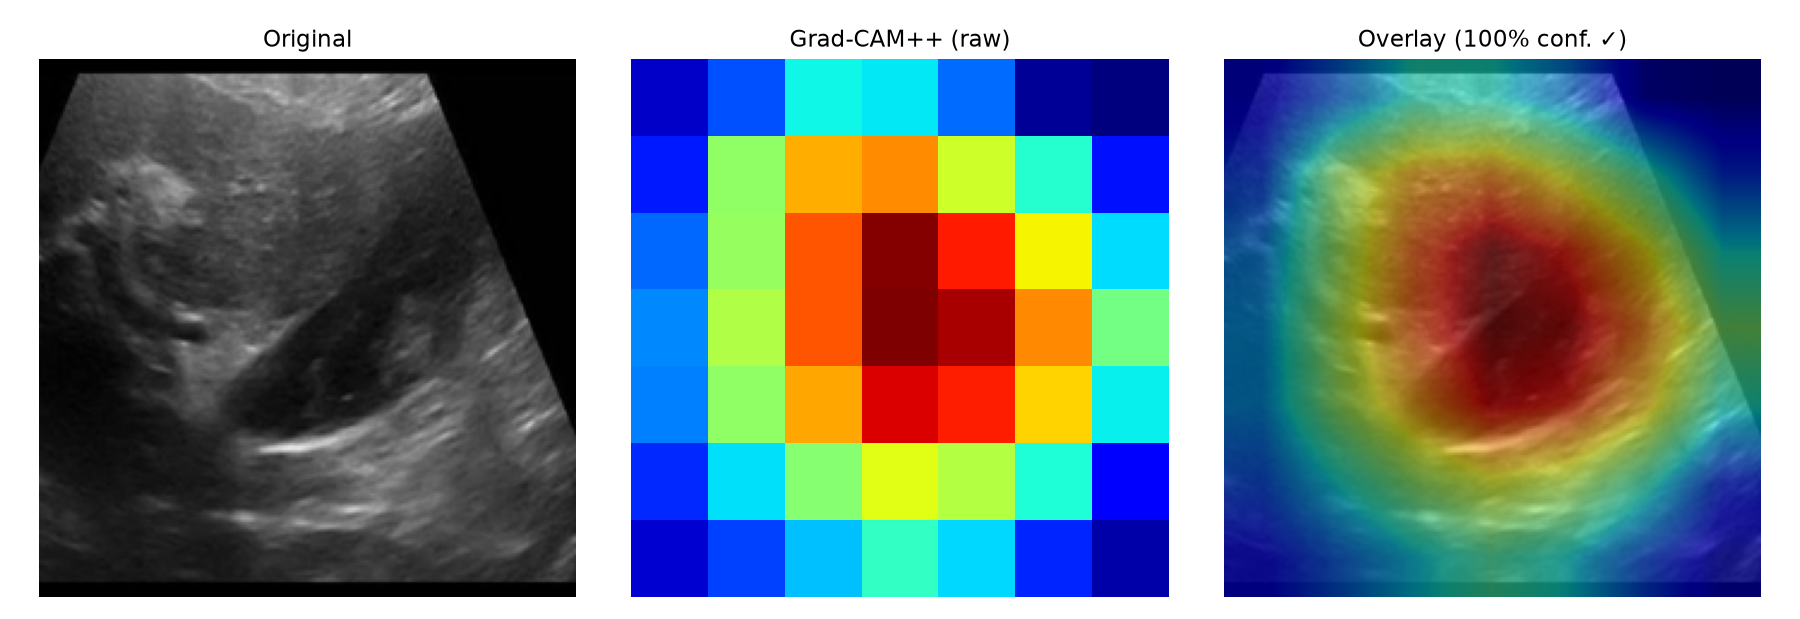
\includegraphics[width=0.48\linewidth]{figures/fig7_expanded/08_carcinoma_02}\hfill
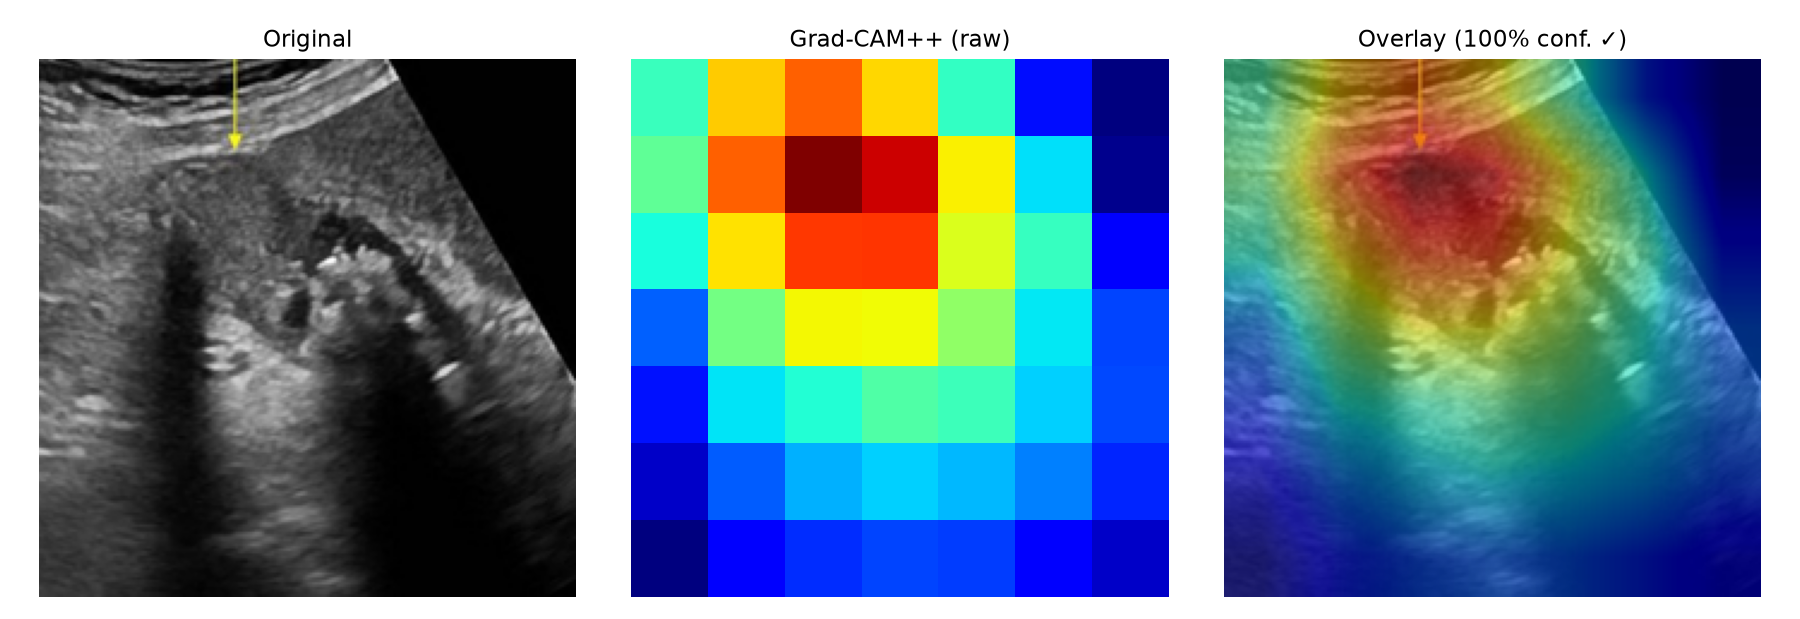
\includegraphics[width=0.48\linewidth]{figures/fig7_expanded/08_carcinoma_03}\\[2pt]
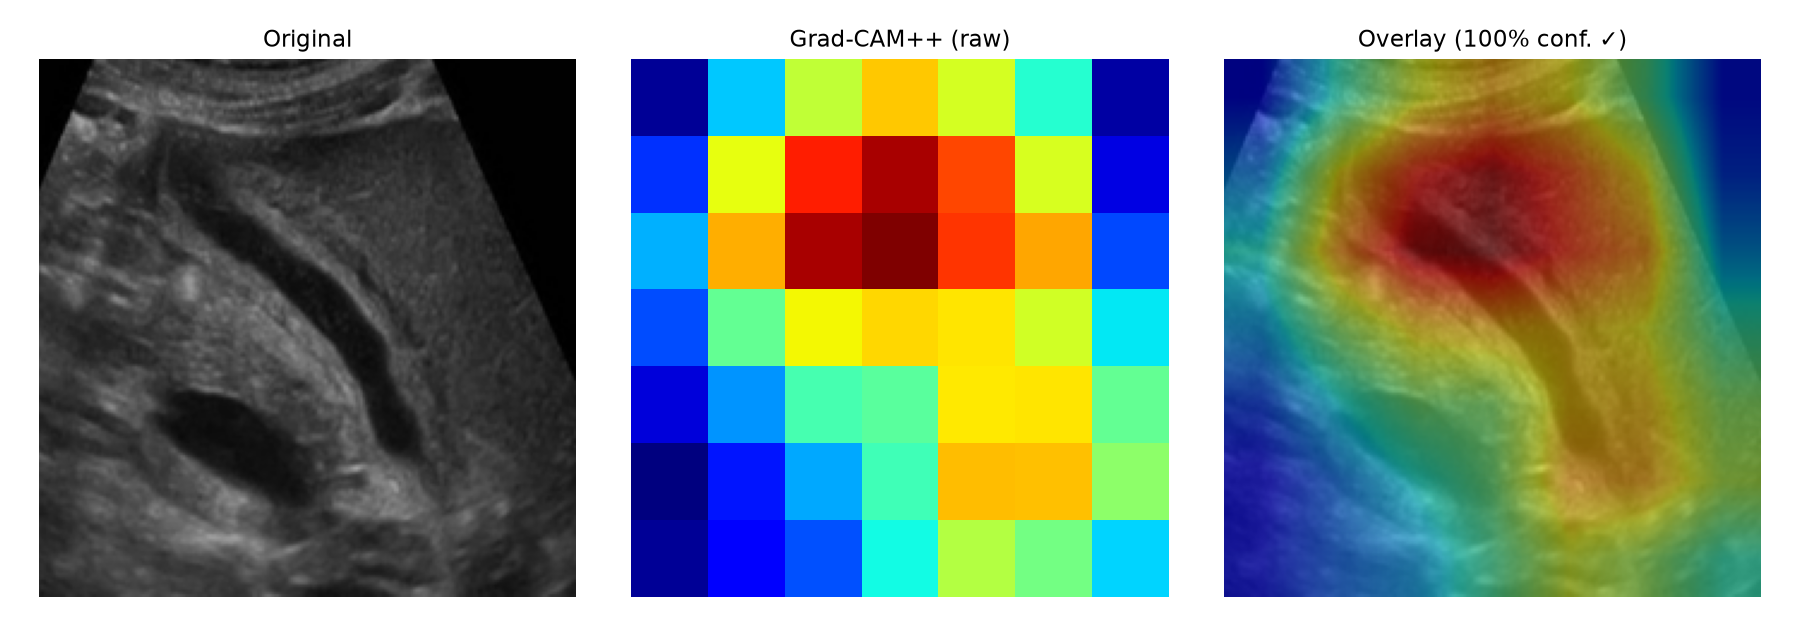
\includegraphics[width=0.48\linewidth]{figures/fig7_expanded/09_various_causes_of_gallbladder_wall_thickening_01}\hfill
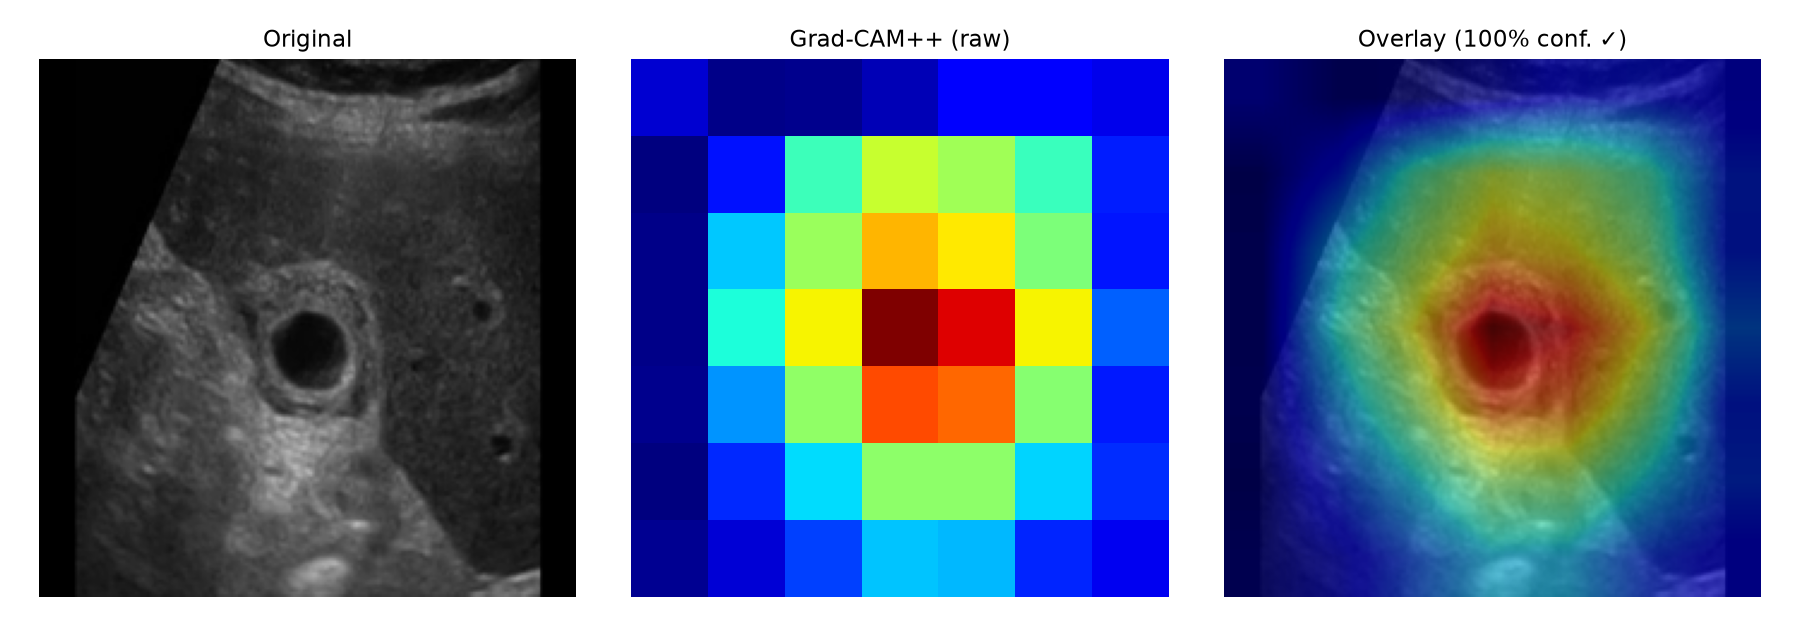
\includegraphics[width=0.48\linewidth]{figures/fig7_expanded/09_various_causes_of_gallbladder_wall_thickening_02}
\caption{Continued from Fig.~\ref{fig:8}: the remaining representative images for Perforation, Polyps \& Cholesterol Crystals, Adenomyomatosis, Carcinoma (three samples, the largest class), and Wall Thickening. Together, Figs.~\ref{fig:8}--\ref{fig:8b} cover all nine classes with 2--3 independent samples each (20 images total), confirming the heatmap patterns described above generalise across images within each class rather than reflecting one cherry-picked example.}
\label{fig:8b}
\end{figure*}

\textit{XAI Finding (4):} For Carcinoma, Grad-CAM++ and Score-CAM produce sharper, more localised wall-region attention than standard Grad-CAM. This is consistent with the expected discriminative feature for malignancy (focal wall irregularity and thickening) and makes Grad-CAM++ a strong candidate for subsequent clinician validation on this class, given its high cross-training consistency (Section~\ref{sec:results}.3) alongside competitive faithfulness (Section~\ref{sec:results}.4); this is not, absent clinician ROI validation and given Grad-CAM's comparable faithfulness score, a claim that Grad-CAM++ is the preferred visualisation method for malignancy detection in general.

\textit{XAI Finding (5):} Quantitatively, the mean cosine consistency $O_r^c$ between the primary and replicate-model Grad-CAM heatmaps across all classes and replicates is \textbf{0.769} (72 stratified validation images $\times$ 3 replicates, Section~\ref{sec:methods}.3), with wide variance across replicates (0.898, 0.629, 0.781). Grad-CAM++ and Score-CAM are both far higher and far more stable (macro mean 0.944 and 0.937 respectively). This indicates those two methods' explanations are the most consistent property of the learned decision boundary under the cross-training-replicate design of Section~\ref{sec:methods}.3---in which the replicate models are trained on disjoint subsets of the corrected training set, so the measured consistency reflects robustness to combined re-initialisation and moderate class-distribution shift, not isolated stochastic-seed variance on identical training data (Section~\ref{sec:limitations}).

\begin{table*}[!ht]
\centering
\caption{Cosine-Consistency Scores $O_r^c$ per XAI Method, Primary Model vs. Each of Three Replicates, over a Stratified 72-Image Evaluation Set (8/class~$\times$~9 classes, seed~=~42). Threshold $\theta=0.70$ flags divergent cases; best macro mean in bold. Eigen-CAM's low score reflects a mismatch between a class-agnostic method and this class-conditional metric (see note below the table), not a reliability finding comparable to the other four methods.}
\label{tbl:5}
\begin{tabular}{lccccc}
\toprule
Method & $R_1$ $O_1^c$ & $R_2$ $O_2^c$ & $R_3$ $O_3^c$ & Macro Mean~$\pm$~Std & Bootstrap 95\% CI \\
\midrule
Grad-CAM & 0.898 & 0.629 & 0.781 & 0.769~$\pm$~0.314 & $[0.735,\,0.803]$ \\
Grad-CAM++ & 0.948 & 0.935 & 0.948 & \textbf{0.944~$\pm$~0.044} & $[0.935,\,0.950]$ \\
Saliency Map & 0.686 & 0.669 & 0.689 & 0.681~$\pm$~0.037 & $[0.675,\,0.687]$ \\
Eigen-CAM & 0.280 & 0.227 & 0.220 & 0.242~$\pm$~0.343 & $[0.174,\,0.314]$ \\
Score-CAM & 0.939 & 0.934 & 0.937 & 0.937~$\pm$~0.051 & $[0.929,\,0.944]$ \\
\bottomrule
\end{tabular}

\vspace{2pt}
\raggedright\footnotesize Computed between the primary model and each of three independently trained replicate models (Section~\ref{sec:methods}.3) over the same stratified 72-image set for every method. Bootstrap 95\% CIs use 2,000 image-level resamples (with replacement) of the macro mean, added in response to a review noting no XAI table in the paper carried a confidence interval; note that Grad-CAM++'s and Score-CAM's intervals do not overlap Grad-CAM's, Saliency's, or Eigen-CAM's, supporting the claim that their consistency advantage is not merely noise at this sample size, while Grad-CAM++'s and Score-CAM's own intervals substantially overlap each other. This quantifies explanation reproducibility only; it is not a measure of diagnostic or localization correctness, which requires clinician-annotated regions of interest (Section~\ref{sec:future-research}). \textit{Eigen-CAM caveat:} Eigen-CAM is class-agnostic by construction (Section~\ref{sec:methods}.3): its output does not condition on the explained class $c$ at all, so it computes the same dominant-activation map regardless of which class is being explained. The $O_r^c$ metric compares heatmaps produced \textit{for a specific class}, a criterion Eigen-CAM's design does not target. Its low score here is therefore a mismatch between a class-conditional metric and a class-agnostic method, not direct evidence that Eigen-CAM's explanations are less reliable than the other four; a fair reliability comparison for Eigen-CAM would require a class-agnostic consistency measure, which this paper does not compute.
\end{table*}

\begin{table*}[!ht]
\centering
\caption{Cosine-Consistency Mean $\bar{O}^c$ per Class, Compared Across All Five XAI Methods (Averaged over $R_1$, $R_2$, $R_3$; Stratified 72-Image Evaluation Set, seed~=~42). Best method per class in bold.}
\label{tbl:6}
\begin{tabular}{lccccc}
\toprule
Class & Grad-CAM & Grad-CAM++ & Saliency Map & Eigen-CAM & Score-CAM \\
\midrule
Gallstones (GS) & 0.595 & \textbf{0.932} & 0.651 & 0.271 & 0.928 \\
Abdomen \& Retroperitoneum (ART) & 0.850 & 0.941 & 0.702 & 0.255 & \textbf{0.934} \\
Cholecystitis (CHOL) & 0.860 & \textbf{0.943} & 0.670 & 0.333 & 0.943 \\
Membranous/Gangrenous Cholecystitis (MGC) & 0.727 & \textbf{0.959} & 0.681 & 0.073 & 0.931 \\
Perforation (PERF) & 0.749 & \textbf{0.941} & 0.678 & 0.379 & 0.932 \\
Polyps \& Cholesterol Crystals (PCC) & 0.873 & \textbf{0.959} & 0.697 & 0.526 & 0.956 \\
Adenomyomatosis (ADNM) & 0.895 & 0.939 & 0.688 & 0.085 & \textbf{0.943} \\
Carcinoma (CARC) & 0.742 & \textbf{0.917} & 0.686 & 0.192 & 0.911 \\
Wall Thickening (WT) & 0.630 & 0.962 & 0.680 & 0.066 & \textbf{0.953} \\
\midrule
\textbf{Macro Mean} & 0.769 & \textbf{0.944} & 0.681 & 0.242 & 0.937 \\
\bottomrule
\end{tabular}

\vspace{2pt}
\raggedright\footnotesize Grad-CAM++ achieves the highest macro-mean consistency overall ($\bar{O}^c=0.944$) and wins six of nine classes; Score-CAM is a close second overall ($\bar{O}^c=0.937$) and wins the remaining three. Both anchor their weighting to the target class's evidence---Grad-CAM++ via second-order gradient weighting, Score-CAM via each channel's actual effect on the softmax score---avoiding the gradient saturation/noise that can affect plain Grad-CAM, which is far more volatile ($\bar{O}^c=0.769\pm0.314$) and collapses for Gallstones and Wall Thickening (0.595, 0.630); Saliency Maps' finer pixel-space granularity similarly makes small per-model differences contribute disproportionately to cosine divergence ($\bar{O}^c=0.681$). Neither pattern should be read as evidence these two methods' explanations are less clinically meaningful, only less reproducible across retraining under this design. Eigen-CAM's near-zero score ($\bar{O}^c=0.242$, falling below 0.10 for three classes) is excluded from this ranking-by-magnitude reading entirely: as Table~\ref{tbl:5}'s note explains, Eigen-CAM is class-agnostic and this metric is class-conditional, so its low score reflects that mismatch rather than a genuine reliability deficit comparable to the other four methods.
\end{table*}

\begin{figure*}[!ht]
\centering
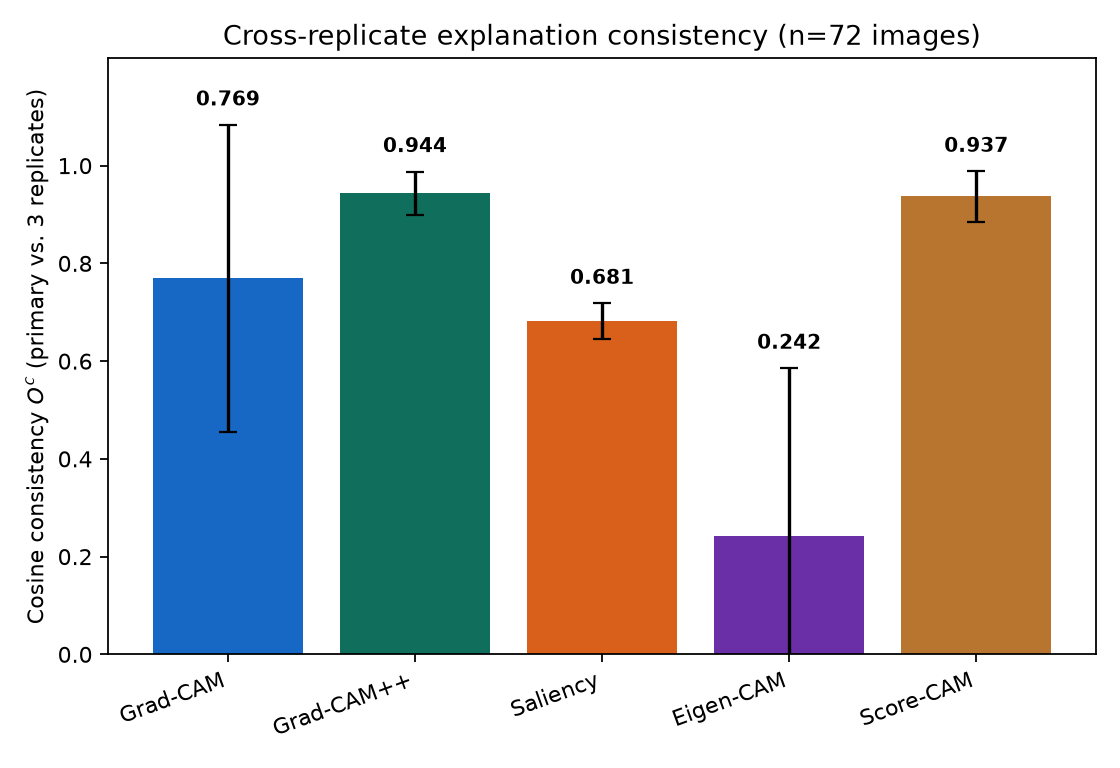
\includegraphics[width=0.55\textwidth]{figures/consistency.png}
\caption{Visual companion to Table~\ref{tbl:5}: macro cosine-consistency mean~$\pm$~std for each of the five XAI methods (72-image stratified set, three replicates). Grad-CAM++ and Score-CAM cluster tightly near 0.94; Grad-CAM shows the widest error bar of the three CAM-family methods; Eigen-CAM is both lowest and most volatile.}
\label{fig:9}
\end{figure*}

Table~\ref{tbl:6} reveals three consistent patterns. First, Grad-CAM++ and Score-CAM stay above $\theta=0.70$ for all nine classes, while plain Grad-CAM drops below threshold for two classes it would otherwise be expected to handle well (Gallstones 0.595, Wall Thickening 0.630), suggesting Grad-CAM's coarser, unweighted feature-map averaging, rather than class difficulty, is the limiting factor. Second, Eigen-CAM collapses almost completely for Membranous/Gangrenous Cholecystitis, Adenomyomatosis, and Wall Thickening ($\bar{O}^c=0.073$, $0.085$, $0.066$), consistent with these three classes having the most diffuse, least focal discriminative regions (Section~\ref{sec:results}.3), which leaves Eigen-CAM's unsupervised principal component with the least consistent direction to lock onto across training subsets. Third, Grad-CAM's per-replicate breakdown (Table~\ref{tbl:5}: 0.898, 0.629, 0.781) shows replicate $R_2$, trained on the smallest subset (2,089~images), diverging most from the primary model, whereas Grad-CAM++ and Score-CAM stay tightly clustered regardless of subset size: the two best methods are also the most robust to training-data volume.

\subsection{Quantitative reliability battery}

\textbf{Faithfulness.} Cross-replicate consistency (Section~\ref{sec:results}.3) establishes that explanations are reproducible, but not that they are \textit{faithful}, in the sense that the highlighted pixels are the ones the model actually relies on. Faithfulness is tested directly with deletion and insertion curves \cite{ref14}: starting from each validation image, the most-attributed pixels are progressively replaced with a blurred baseline (deletion, where a faithful map makes the predicted-class probability fall fast, so \textit{lower} area-under-curve is better), and separately restored onto a blurred baseline (insertion, where a faithful map makes probability rise fast, so \textit{higher} AUC is better). Each method is compared against a random pixel-ordering control on the same 144 stratified images (20 removal/insertion steps). This test is run for the three methods that anchor their weighting to the target class's evidence in feature-map space (Grad-CAM, Grad-CAM++, Score-CAM); Eigen-CAM is excluded because it is class-agnostic and so has no class-specific attribution ordering for this test to remove or restore, and Saliency Maps are excluded because they attribute in raw pixel space rather than the feature-map space the deletion/insertion baseline masking here assumes, making a direct three-way comparison with the CAM-family methods not straightforwardly meaningful.

\begin{table}[!ht]
\centering
\caption{Deletion / Insertion Faithfulness (144 stratified validation images, 20 steps). Lower deletion AUC and higher insertion AUC are better; the gap (insertion~$-$~deletion) is a single faithfulness score. All three CAM methods beat the random control by a wide margin. Eigen-CAM and Saliency Maps are not included; see the exclusion rationale above.}
\label{tbl:7}
\begin{tabular}{lcccc}
\toprule
Method & Deletion AUC~$\downarrow$ & Insertion AUC~$\uparrow$ & Gap~$\uparrow$ & Gap Bootstrap 95\% CI \\
\midrule
Grad-CAM & 0.307 & \textbf{0.787} & \textbf{0.480} & $[0.437,\,0.518]$ \\
Grad-CAM++ & \textbf{0.312} & 0.785 & 0.473 & $[0.430,\,0.515]$ \\
Score-CAM & 0.323 & 0.778 & 0.456 & $[0.413,\,0.498]$ \\
Random control & 0.610 & 0.597 & $-0.013$ & $[-0.024,\,-0.004]$ \\
\bottomrule
\end{tabular}

\vspace{2pt}
\raggedright\footnotesize Gap bootstrap 95\% CIs use 2,000 image-level resamples (with replacement), added in response to a review noting the close three-way faithfulness ranking (0.480 vs.\ 0.473 vs.\ 0.456) had no interval showing whether it was distinguishable from noise: all three CAM methods' intervals overlap substantially, confirming the ranking should not be over-interpreted, exactly as XAI Finding~(6) already states qualitatively. The random control's interval excludes zero but remains far below all three CAM methods, the expected null result.
\end{table}

\begin{figure*}[!ht]
\centering
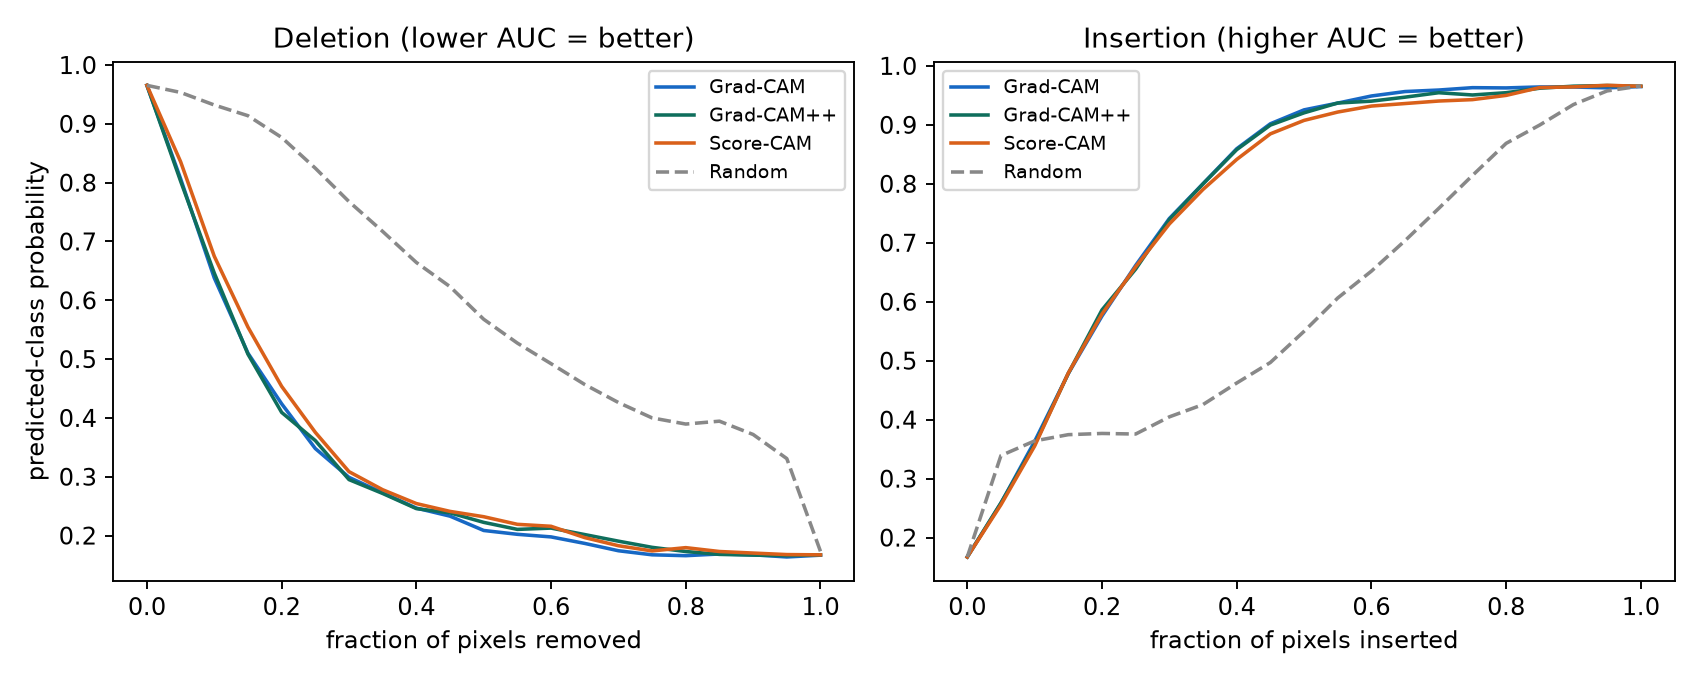
\includegraphics[width=0.7\textwidth]{figures/faithfulness.png}
\caption{Mean deletion (left) and insertion (right) curves. All three CAM methods sit far below the random control under deletion and far above it under insertion, confirming their heatmaps are faithful to the model's decision rather than merely plausible. The random control's near-zero gap (Table~\ref{tbl:7}) is the expected null result.}
\label{fig:10}
\end{figure*}

\textit{XAI Finding (6):} All three CAM-family methods are faithful by the deletion/insertion criterion, each beating the random control by a wide margin (gap 0.46--0.48 vs. $-0.013$). The three-way ranking among them (Grad-CAM 0.480, Grad-CAM++ 0.473, Score-CAM 0.456) is too close to over-interpret. This quantitative result, not the visual plausibility of the Section~\ref{sec:results}.2 failure-case heatmaps, is what licenses trusting the explanations.

\textbf{Stability.} A reliable explanation should not shift substantially under image perturbations that are intended to be diagnostically minor. Three candidate transforms are applied to 216 stratified validation images: a $\times1.15$ brightness shift, a 10-pixel diagonal translation (heatmap realigned before comparison), and additive Gaussian noise ($\sigma=0.03$). As the prediction-retention column of Table~\ref{tbl:8} below shows, though, not all three actually leave the classifier's own prediction unchanged; only brightness does so reliably. For each transform, Grad-CAM++ is recomputed for the originally predicted class, and agreement with the unperturbed heatmap is measured via SSIM, Pearson correlation, and top-10\% pixel overlap (IoU), together with the fraction of images whose predicted class is unchanged. Because prediction changes and explanation changes are conflated whenever a transform is not prediction-preserving, the headline SSIM/Pearson/IoU numbers below should be read as agreement over all 216 images regardless of whether the prediction held; XAI Finding~(7) separates the two effects explicitly for the noise transform, where the distinction matters most.

\begin{table}[!ht]
\centering
\caption{Grad-CAM++ Explanation Stability Under Candidate Minor-Perturbation Transforms (216 stratified validation images). ``Pred. kept'' shows only brightness is reliably prediction-preserving; translation and noise are not.}
\label{tbl:8}
\begin{tabular}{lcccc}
\toprule
Transform & SSIM (95\% CI) & Pearson & Top-10\% IoU & Pred. kept \\
\midrule
Brightness ($\times1.15$) & \textbf{0.995} $[0.994,0.995]$ & \textbf{0.998} & \textbf{0.907} & \textbf{98.6\%} \\
Translation (10~px) & 0.848 $[0.845,0.852]$ & 0.931 & 0.681 & 93.5\% \\
Gaussian noise ($\sigma=0.03$) & 0.931 $[0.926,0.936]$ & 0.950 & 0.652 & 70.8\% \\
\bottomrule
\end{tabular}

\vspace{2pt}
\raggedright\footnotesize SSIM 95\% CIs use 2,000 image-level bootstrap resamples, added in response to a review noting no XAI table carried a confidence interval; all three transforms' SSIM intervals are narrow and non-overlapping, so the brightness/translation/noise ranking in this column is well-supported at this sample size. Pearson and top-10\% IoU bootstrap 95\% CIs (also computed, narrow in every case, e.g.\ Pearson brightness $[0.997,\,0.998]$, translation $[0.923,\,0.937]$, noise $[0.942,\,0.957]$; top-10\% IoU brightness $[0.896,\,0.917]$, translation $[0.659,\,0.704]$, noise $[0.627,\,0.676]$) are omitted from the table for space but available in \texttt{outputs/phase0/stability.json}.
\end{table}

\begin{figure*}[!ht]
\centering
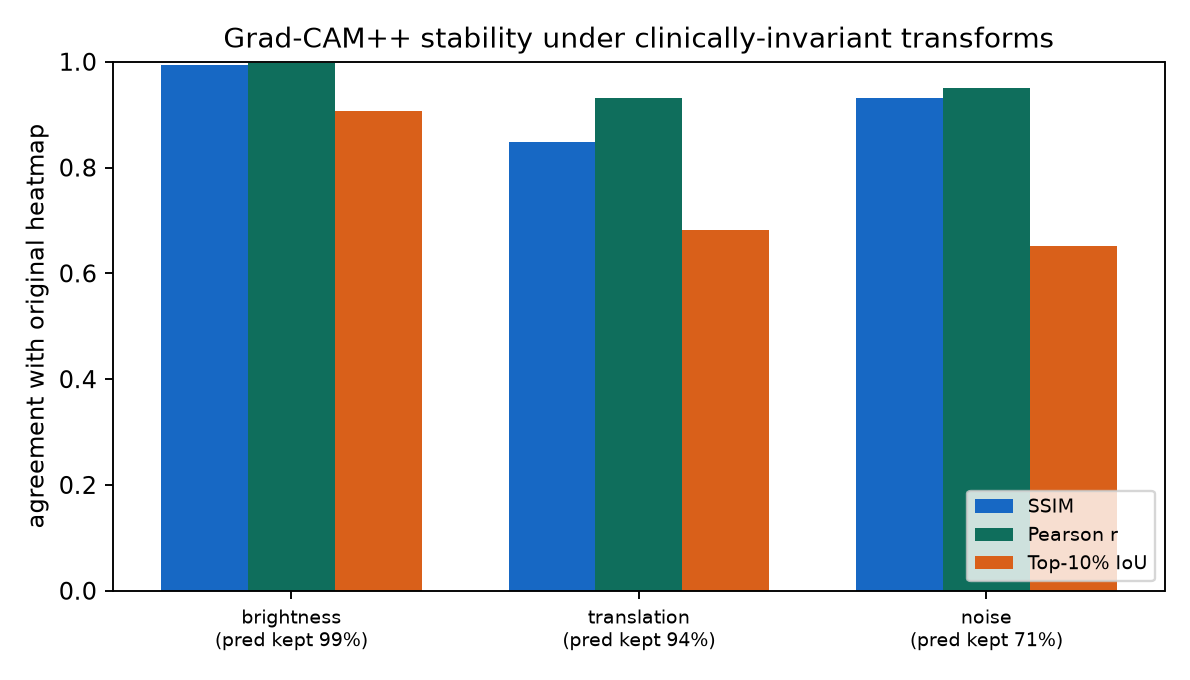
\includegraphics[width=0.6\textwidth]{figures/stability.png}
\caption{Grad-CAM++ explanation stability under the three transforms. Brightness is near-perfectly stable on every axis; translation and noise diverge---translation disturbs the heatmap's pixel-level structure (lowest SSIM) more than noise does, while noise disturbs the model's actual prediction (lowest prediction-kept rate) far more than translation does.}
\label{fig:11}
\end{figure*}

\textit{XAI Finding (7):} Grad-CAM++ is highly stable under brightness change (SSIM~0.995, prediction kept 98.6\%), but translation and noise disrupt different things. Translation degrades the heatmap most (SSIM~0.848) while leaving the prediction largely intact (93.5\% kept). Noise leaves the heatmap comparatively more intact (SSIM~0.931) but flips the predicted class nearly 30\% of the time (70.8\% kept). Since noise changes what the model outputs, not just how it explains that output, classifier-level noise robustness---not explanation robustness---is the more urgent target for future training.

\textbf{Model-parameter randomization sanity check.} A trustworthy saliency method must depend on the model's learned weights, yet some popular methods notoriously do not \cite{ref13}. Following the Adebayo et~al. protocol, ResNet-50's parameters are cascade-randomized from the output layer back toward the input (fc~$\rightarrow$~layer4~$\rightarrow$~$\dots$~$\rightarrow$~conv1), Grad-CAM++ is recomputed for the same explained class at each stage, and similarity to the fully-trained-model heatmap is measured (108 images). As Fig.~\ref{fig:12} shows, similarity is highest when only \texttt{fc} is randomized ($|\rho|=0.95$), which is expected since Grad-CAM++ taps \texttt{layer4} and \texttt{fc} lies downstream of that tap. It then drops sharply as soon as \texttt{layer4} itself is randomized ($|\rho|=0.52$), keeps falling through \texttt{layer3} and \texttt{layer2}, and reaches its minimum at \texttt{layer1} ($|\rho|=0.20$), with a modest uptick at \texttt{conv1} ($|\rho|=0.33$) that stays far below the trained-model value. The heatmap therefore genuinely depends on the learned convolutional features rather than acting as an input-edge detector, and the method passes the sanity check.

\begin{figure*}[!ht]
\centering
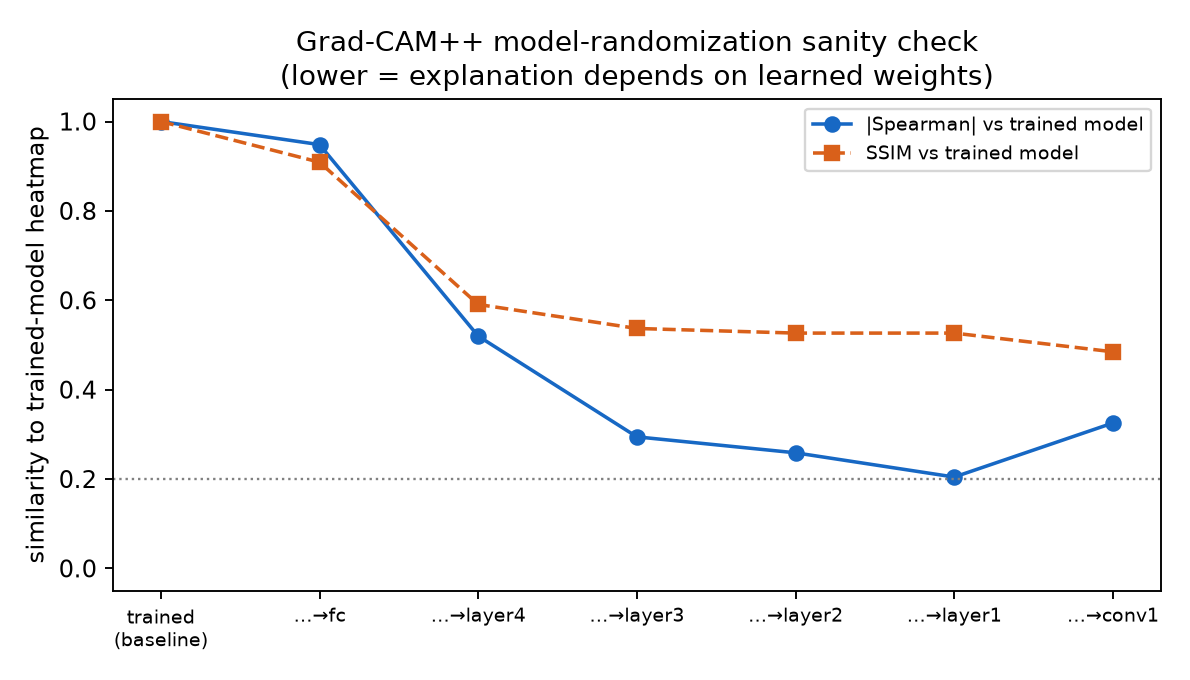
\includegraphics[width=0.6\textwidth]{figures/sanity_checks.png}
\caption{Model-randomization sanity check. Grad-CAM++ heatmap similarity to the trained model (absolute Spearman correlation and SSIM) drops sharply once \texttt{layer4}---the Grad-CAM++ tap point---is randomized and continues declining through the remaining convolutional stages, confirming the explanation reflects learned weights rather than acting as an input-edge detector.}
\label{fig:12}
\end{figure*}

\textbf{Probability calibration.} Unlike the faithfulness, stability, sanity-check, and shortcut-audit results above, calibration is a property of the underlying classifier's confidence output, not of any XAI explanation. It is reported alongside the explanation-reliability battery because both jointly determine whether the model's overall output, prediction, confidence, and explanation together, can be trusted, not because calibration is itself a measure of explanation quality. Section~\ref{sec:results}.2 noted that the model's raw softmax confidence separates correct from incorrect predictions but is not a calibrated probability; that observation is now quantified and corrected. A single temperature parameter \cite{ref42} is fit on a stratified calibration half of the validation set (1,594 images) and evaluated on the held-out half (1,599 images, accuracy~0.9318). Temperature scaling ($T=1.468$) reduces Expected Calibration Error from 0.034 to 0.009 and the Brier score from 0.109 to 0.106, without altering discrimination, since accuracy is unchanged by construction. Fig.~\ref{fig:13} shows the model is mildly over-confident before scaling, with its reliability curve sitting slightly below the diagonal at high confidence, and closely calibrated afterward.

\begin{figure}[!ht]
\centering
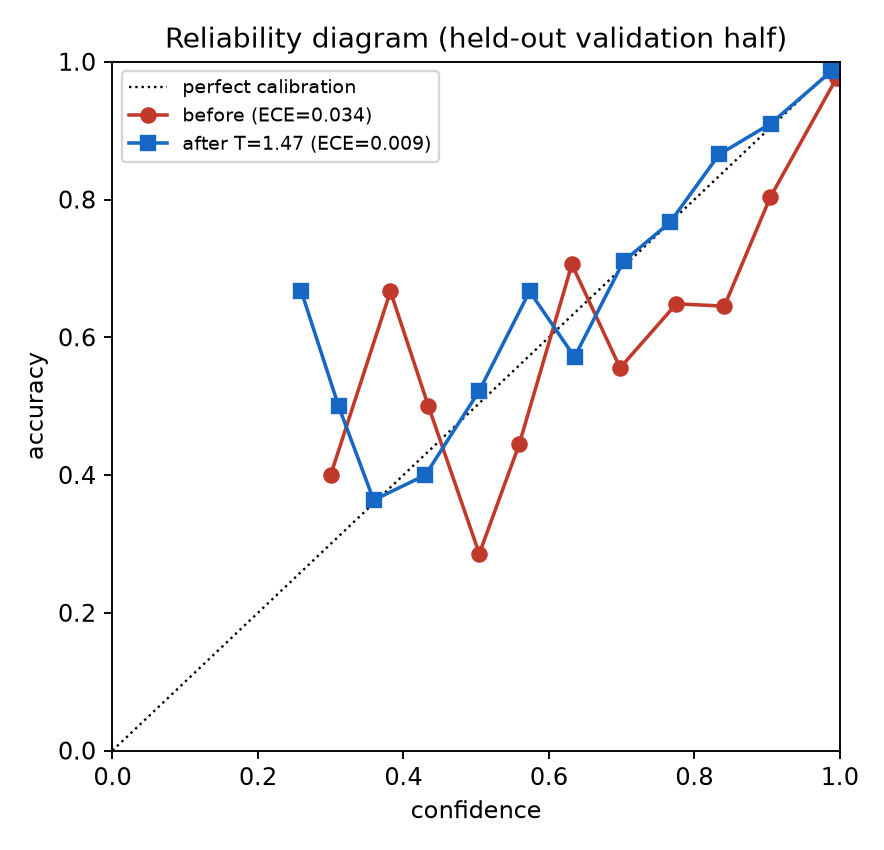
\includegraphics[width=0.85\linewidth]{figures/calibration.png}
\caption{Reliability diagram on the held-out validation half. Temperature scaling ($T=1.468$) moves the confidence--accuracy curve toward the diagonal, cutting ECE by 73\% (0.034~$\rightarrow$~0.009).}
\label{fig:13}
\end{figure}

\textbf{Shortcut-learning audit.} Finally, this section tests one narrow, specific shortcut hypothesis: whether the model exploits non-clinical cues at the image margin (burned-in text, calipers, borders) rather than central image content \cite{ref40}, \cite{ref41}, via two measurements on 216 stratified images (Fig.~\ref{fig:14}). Cropping away the outer 12\% margin and resizing back changes accuracy substantially, from 0.9305 to 0.7122 ($-0.2183$) and macro-F1 from 0.9303 to 0.7039, while only 21.8\% ($\pm$~4.9\%) of Grad-CAM++ attribution mass falls in that margin ring, even though the ring occupies 41.0\% of the frame, markedly \textit{under}-weighted relative to its area. These two measurements point in different directions and are both reported honestly. Attribution mass being under-represented in the margin region provides no strong attribution-level evidence of margin-shortcut reliance, though attribution is not exhaustive proof of causal non-reliance. The much larger accuracy drop is not, on its own, evidence of margin-shortcut reliance either, and the crop-ablation result should be interpreted cautiously: a 12\% crop removes genuine peripheral gallbladder and adjacent-organ anatomy along with any border artefact, and for a nine-class task with several visually similar classes (Section~\ref{sec:results}.2) losing that anatomy plausibly costs real discriminative signal independent of any shortcut, confounding the two possible explanations for the drop. The crop-accuracy drop is therefore treated as a robustness finding rather than clean evidence of shortcut learning, with the border-energy result treated as the actual, narrow, margin-only shortcut audit. This audit does not test for, and does not rule out, other shortcuts a classifier could in principle learn: scanner-specific artefacts, hospital- or site-correlated imaging conventions, compression artefacts, or other background cues not tied to the image margin specifically.

\begin{figure*}[!ht]
\centering
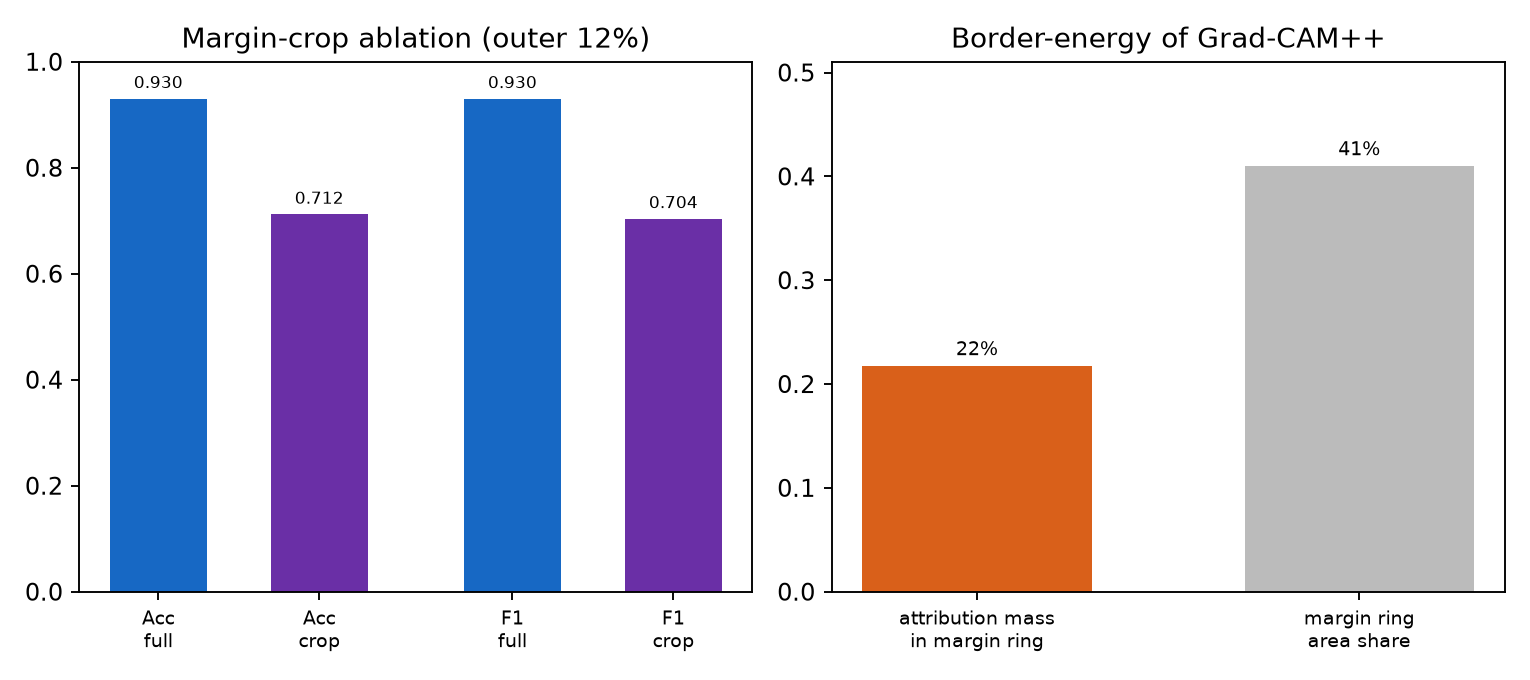
\includegraphics[width=0.65\textwidth]{figures/shortcut_audit.png}
\caption{Shortcut audit. Left: classification accuracy and macro-F1 both drop substantially under the outer-12\%-margin crop. Right: Grad-CAM++ places only 21.8\% of its attribution mass in that margin ring (which covers 41.0\% of the frame), indicating central-anatomy focus in the explanation even though the crop itself is costly to accuracy.}
\label{fig:14}
\end{figure*}

\textit{XAI Finding (8):} Attribution mass is markedly under-represented at the frame margin (21.8\% of mass in a 41.0\%-area ring), evidence against margin-shortcut reliance. The much larger crop-ablation accuracy drop (0.930~$\rightarrow$~0.712) is interpreted as genuine peripheral-anatomy dependence rather than a shortcut the border-energy measurement missed, but this is the one reliability result in the paper that is not fully clean (Section~\ref{sec:future-research}).

\subsection{Summary of key findings}

Three findings carry across Sections~\ref{sec:results}.1--4. Grad-CAM++ and Score-CAM lead on cross-replicate consistency, the reliability axis with the clearest separation between methods, but that lead does not carry over to faithfulness, where all three CAM-family methods are comparable and plain Grad-CAM numerically edges out the other two, so no method leads on every axis measured. The explanations are quantitatively faithful to the model's decision, yet heatmap plausibility alone flags neither high-confidence errors (Section~\ref{sec:results}.2) nor subtler failure modes in general, so reliability has to be measured rather than inferred from appearance. Of the reliability axes, only the shortcut audit is inconclusive, for the crop-versus-anatomy reason given in Section~\ref{sec:results}.4.

\subsection{Stage 2: cluster-aware split with a genuine held-out test set}
\label{sec:stage2}

The results above (Sections~\ref{sec:results}.1--4) come from the Stage~1 pipeline: images de-duplicated by single-orientation perceptual hashing (Section~\ref{sec:methods}.1), then split 70/30 into training and validation, with every number in this paper reported on that validation set. A subsequent, independent audit found this correction incomplete in two ways. First, 96.73\% of images share a filename-prefix ``session'' that the Stage~1 split did not keep together, so near-identical frames from the same imaging session could land on both sides of the train/validation boundary. Second, the dataset's own source publication confirms images were released after augmentation by rotation, flipping, and brightness/contrast/saturation jitter, and a rotation-aware (dihedral) hash re-check found 46\% of the corpus (4,918 of 10,692 images) has at least one cross-split duplicate that single-orientation hashing could not detect.

A Stage~2 pipeline addresses both gaps together. Every image is assigned to a duplicate cluster using an 8-orientation (dihedral) perceptual hash (1,570 clusters from the full 10,692-image corpus), and the corpus is re-split at the cluster level, 70/20/10, so no cluster crosses a train/validation/test boundary and, unlike Stage~1, a test set is held out and touched exactly once, after every other design decision (epoch budget, early-stopping criterion) is already frozen. This yields 7,470 training, 2,138 validation, and 1,084 test images. A primary model (seed~42) and three replicate models (seeds~7, 123, 2027) are trained on the identical 7,470-image training set, varying only the random seed and data-loader shuffling order---correcting the Stage~1 replicate design, in which the three replicates were trained on disjoint subsets of 2,749, 2,089, and 2,661 images respectively and therefore could not isolate seed-to-seed reproducibility from data-composition effects (Limitation~2b). Training uses up to 20 epochs with early stopping on validation macro-F1 (patience~5), rather than Stage~1's fixed 10-epoch budget.

\begin{table}[!ht]
\centering
\caption{Stage 2: Held-Out Test Performance, Cluster-Aware 70/20/10 Split (Test $n=1084$). All four models see identical training data; only the random seed varies.}
\label{tbl:stage2-test}
\begin{tabular}{lccc}
\toprule
Model & Test Accuracy & Macro-F1 & Epochs to best \\
\midrule
Primary (seed~42) & 0.7030 & 0.7039 & --- \\
Replicate (seed~7) & 0.7020 & 0.6992 & --- \\
Replicate (seed~123) & 0.7482 & 0.7486 & --- \\
Replicate (seed~2027) & 0.7491 & 0.7438 & --- \\
\midrule
\textbf{Mean~$\pm$~Std} & \textbf{0.7256~$\pm$~0.0235} & \textbf{0.7239~$\pm$~0.0221} & \\
\bottomrule
\end{tabular}
\end{table}

Table~\ref{tbl:stage2-test} reports the real, unbiased test performance this design supports: a four-model mean accuracy of 72.56\%~$\pm$~2.35\% and macro-F1 of 72.39\%~$\pm$~2.21\%, all four seeds agreeing within roughly a five-point band. This is substantially lower than the Stage~1 headline of 93.05\% accuracy, and it is the more trustworthy of the two numbers precisely because Stage~1's validation set was not fully protected from cluster-level leakage. It is also markedly higher than the 29.59\% single-run figure produced by an earlier, more aggressive session-level-only correction (Section~\ref{sec:limitations}), which re-split the existing Stage~1 train/validation files at the filename-session level without also addressing the rotation-augmented-duplicate gap or retraining with a longer schedule; that figure should be read as a lower bound from an under-specified re-split rather than the pipeline's ceiling. The Stage~2 result in Table~\ref{tbl:stage2-test} is the paper's best current estimate of what this classifier, honestly evaluated, actually achieves on nine-class gallbladder ultrasound classification.

\textit{XAI Finding (9): the null-control test for the consistency metric.} A structural concern raised against the Stage~1 consistency scores in Table~\ref{tbl:5} is that Grad-CAM-family heatmaps end in a ReLU and are then min-max normalised to $[0,1]$, so two \textit{unrelated} non-negative heatmaps of the same shape may already have high cosine similarity as a mathematical artefact, independent of anything the model has learned. Two null controls quantify this floor directly. First, cross-model consistency is measured between four \textit{untrained} ResNet-50 models (ImageNet backbone, randomly initialised nine-class head, no fine-tuning): mean cosine similarity $0.333\pm0.231$ over 240 pairwise comparisons across 40 stratified test images. Second, cosine similarity is measured between pairs of purely synthetic heatmaps with no model, image, or learning involved: $0.755\pm0.044$ for independent uniform-random $[0,1]$ maps, and $0.325\pm0.107$ for ReLU-thresholded standard-Gaussian noise, min-max normalised the same way Grad-CAM's own output is---the more representative control, since it reproduces Grad-CAM's actual non-linearity rather than assuming uniform noise. Against this pair of floors ($0.33$ untrained-model, $0.33$ ReLU-Gaussian-synthetic), the Stage~2 same-data cross-replicate consistency of $0.848$, $0.816$, and $0.863$ (mean $\approx0.843$, per-replicate-mean std $=0.0196$; Section~\ref{sec:results}.3's Grad-CAM++ score, recomputed under the corrected same-data replicate design of this section) clears both floors by roughly a factor of 2.5, rather than sitting close to them. The consistency claim therefore survives the null-control test the metric had not previously been checked against, though this recomputation used Grad-CAM specifically as the representative CAM-family method, not the full five-method comparison of Table~\ref{tbl:5}, and the uniform-random floor of $0.755$---higher than either the untrained-model or ReLU-Gaussian floor---shows the choice of null distribution itself matters and should be reported alongside any future consistency claim, not assumed.

The Stage~2 per-replicate-mean standard deviation reported above ($0.0196$) also corrects a labelling error in the Stage~1 tables. Table~\ref{tbl:5}'s std column was computed by pooling every individual image-level score across all three replicates and taking the standard deviation of that pooled set, not the standard deviation of the three replicate-level \textit{means} the table and its caption describe. Recomputed the way the caption implies, the three Stage~2 replicate means $\{0.848, 0.816, 0.863\}$ give a std of $0.0196$; the pooled-image-level std over the same data is $0.186$, an order of magnitude larger. Both quantities are legitimate to report, but they answer different questions---how much do the three replicates' \textit{average} agreement levels differ from one another, versus how much does agreement vary image-to-image within a replicate---and only the first is a std-of-means in the sense Table~\ref{tbl:5}'s caption claims.

\subsection{Follow-up audits: threshold sensitivity, batch-shortcut re-verification, and noise robustness}
\label{sec:followup-audits}

Five remaining review points required new measurements rather than re-analysis of existing results: whether the filename-prefix-as-acquisition-batch inference used throughout this paper is itself supported by evidence beyond the filename pattern, the pHash clustering threshold's sensitivity, whether the batch-ID shortcut diagnostic was itself leakage-free, whether the batch signature is recoverable from the disease classifier's own features (not just a separately-trained proxy), and how classification accuracy, not just explanation stability, degrades under noise. All five are addressed here using the same dihedral cluster manifest and Stage~2 primary checkpoint as the sections above.

\textbf{Direct evidence for the filename-prefix-as-acquisition-session inference.} Section~\ref{sec:methods}.1's batch/session inference (a filename prefix denotes one contiguous acquisition or export session) was previously argued only from filename structure: prefixes follow a consistent pattern, indices are contiguous within a prefix, and no prefix spans two disease-class folders. A reviewer correctly noted this argument is partly circular, since prefixes assigned per class folder at export time would trivially satisfy the single-class property regardless of whether they reflect genuine acquisition sessions. Every one of the 10,692 released images carries embedded EXIF metadata (all exported via ACDSee~Pro~6, per the embedded software tag), including a DateTimeOriginal timestamp, which provides direct, non-inferred evidence independent of the filename pattern itself. Grouping images by filename prefix and examining each group's embedded timestamp range shows a median within-prefix capture-time span of just 5.7 minutes (220 prefixes with usable EXIF data), consistent with one short imaging or export session. More decisively, comparing every pair of prefixes that occur on the same calendar day for whether their time windows overlap at all finds \textbf{zero overlapping pairs out of 3,312 same-day prefix pairs checked}: no two filename-prefix groups ever share a moment in time. This is inconsistent with prefixes being an arbitrary per-class export label, which would be expected to produce interleaved or overlapping time windows across prefixes, and is instead direct evidence that each prefix corresponds to its own distinct, temporally exclusive acquisition or export session. Thirteen of the 220 prefixes (5.9\%) have longer spans exceeding one hour, three of them substantially so (5.8, 7.1, and 7.7 hours), which we report rather than exclude; these may reflect sessions with a genuine pause, batched review-and-export rather than continuous capture, or another export-side explanation this metadata alone cannot distinguish. This evidence does not replace contacting the original dataset providers for their actual export convention, which remains unresolved, but it is direct, quantitative, non-circular support for the inference this paper's Stage~2 correction and shortcut audits depend on.

\textbf{pHash threshold sensitivity.} Section~\ref{sec:methods}.1's clustering uses a Hamming-distance threshold of 4 bits, tightened from an initial choice of 8 after threshold~8 produced a single-linkage chaining artefact (a 498-image cluster spanning multiple disease classes, later traced to a chain of transitively-connected near-threshold matches rather than genuine duplicates). Table~\ref{tbl:phash-sweep} reports how the final cluster count and post-veto mixed-class cluster count move as this threshold is swept from 4 to 12 bits, using the same cached dihedral hashes across all five values so the comparison isolates the threshold's effect. The cluster count roughly triples between threshold~4 and threshold~8 (1,570~$\rightarrow$~2,252) and explodes further at threshold~10 (5,121 clusters, median cluster size drops to 1, meaning most images become effective singletons again), while mixed-class clusters, a proxy for false-positive merges, rise from 4 at threshold~4 to 26 at threshold~8. This supports threshold~4 as the more conservative choice: it produces the smallest, most internally-consistent clusters and the fewest cross-class merges, at the cost of a somewhat larger effective sample size than a looser threshold would give. This sweep does not retrain a classifier at each threshold to report Stage~2 accuracy per threshold, which would require up to five full training runs; the cluster-count and mixed-class sensitivity reported here is a lower-cost but real partial answer to that question, not a substitute for it.

\begin{table}[!ht]
\centering
\caption{pHash Clustering Threshold Sensitivity (Hamming distance, dihedral 8-orientation hashing, 10,692 raw images). Threshold 4 is used throughout this paper; thresholds 6--12 are shown for comparison only.}
\label{tbl:phash-sweep}
\begin{tabular}{lccc}
\toprule
Threshold (bits) & Final Clusters & Mixed-Class Clusters & Median Cluster Size \\
\midrule
4 (used here) & 1,570 & 4 & 6 \\
6 & 1,573 & 14 & 6 \\
8 & 2,252 & 26 & 6 \\
10 & 5,121 & 32 & 1 \\
12 & 9,299 & 12 & 1 \\
\bottomrule
\end{tabular}
\end{table}

\textbf{Batch-ID diagnostic, re-verified without cluster leakage.} The batch-correlated-shortcut diagnostic (a $K$-way classifier trained to predict which acquisition batch a Carcinoma image came from, all images sharing one disease label) originally used a random image-level split within each batch, which a review pointed out could let near-duplicate frames from the same acquisition sit on both sides of that split, inflating its reported 100\% accuracy. Re-running the same 10-batch diagnostic with the dihedral cluster manifest applied, so no duplicate cluster crosses the train/validation boundary (608 training, 292 validation images), gives \textbf{82.88\% accuracy} (8.3$\times$ the 10\% chance level), down from the original 100\% but still far above chance. This confirms the review's concern was partly correct, some of the original 100\% figure was inflated by near-duplicate-frame memorisation, while also confirming its underlying conclusion: a substantial, learnable, non-anatomical batch signature remains even under a leakage-controlled split.

\textbf{Held-out-batch generalisation and a linear probe on the disease classifier's own features.} Two further tests target the batch-correlated shortcut directly, since the paper's only other shortcut audit (Section~\ref{sec:results}.4) tests exclusively for margin/border artefacts and cannot, by its own design, detect this one. First, a 6-way batch classifier trained on a subset of batches reaches 90.31\% held-out accuracy on unseen images from those same batches (chance 16.67\%), and its mean top-1 confidence when forced to classify images from four entirely unseen batches (73.45\%) remains substantial relative to its confidence on seen-batch held-out images (89.77\%), suggesting the signature partially generalises across batches rather than being purely a memorised per-batch artefact. Second, and more directly relevant to whether the \textit{disease} classifier itself is affected: a linear probe trained on the Stage~2 primary disease classifier's own \texttt{layer4} features, the same features that classifier uses to make its actual nine-class decision, recovers batch identity with \textbf{74.75\% accuracy} against 6 batches (chance 16.67\%, 4.5$\times$ chance). This is direct evidence that the disease classifier's learned representation itself correlates with batch identity, not merely that a separately-trained classifier is capable of learning it; the shortcut concern therefore extends to the classifier this paper's own XAI battery is evaluating explanations for.

\textbf{Noise robustness, reported as accuracy rather than only explanation stability.} Section~\ref{sec:results}.4's stability test reported that Gaussian noise at $\sigma=0.03$ changes the predicted class on 29.2\% of images under the Stage~1 model, but did not report classifier accuracy directly or sweep beyond that single noise level. Table~\ref{tbl:noise-sweep} reports accuracy and prediction-change rate directly, swept across seven noise levels on the Stage~2 primary checkpoint. Accuracy on clean images is 90.0\% on this 180-image stratified subset; it falls to 68.3\% by $\sigma=0.03$ and to 20.6\%, barely above the 11.1\% chance level, by $\sigma=0.12$, a noise level that remains visually subtle. The fraction of predictions that flip relative to the clean prediction tracks this drop closely (7.2\% at $\sigma=0.01$ rising to 82.2\% at $\sigma=0.12$), confirming the accuracy collapse and the prediction instability are the same underlying phenomenon rather than two independent effects. This is a substantially more severe classifier-level robustness finding than anything in the XAI comparison itself, and, as Section~\ref{sec:results}.4 already notes, classifier-level noise robustness rather than explanation-level stability is the more urgent target for future model development.

\begin{table}[!ht]
\centering
\caption{Noise-Robustness Sweep, Stage 2 Primary Checkpoint (180 stratified images, 20/class). Accuracy and prediction-change fraction both reported directly, closing a gap where only a single $\sigma$ was previously reported.}
\label{tbl:noise-sweep}
\begin{tabular}{lcc}
\toprule
Noise $\sigma$ & Accuracy & Pred.\ Changed from Clean \\
\midrule
0.00 (clean) & 0.900 & --- \\
0.01 & 0.878 & 0.072 \\
0.02 & 0.800 & 0.172 \\
0.03 & 0.683 & 0.328 \\
0.05 & 0.511 & 0.511 \\
0.08 & 0.333 & 0.683 \\
0.12 & 0.206 & 0.822 \\
\bottomrule
\end{tabular}
\end{table}

\section{Discussion}
\label{sec:discussion}

Here we interpret the classification and XAI results from Section~\ref{sec:results}, compare them to earlier studies. And plainly lay out what this work proves and what it does not.

\subsection{Interpretation of results}

The primary model hits 93.05\% accuracy and 0.9965 macro-AUC (Table~\ref{tbl:3}), and a three-seed replication confirms it ($0.9210\pm0.0131$). Unlike the single-centre GBCU dataset studied before, the 6.6-point F1 difference---between Cholecystitis (0.9601) and Perforation (0.8944)---doesn't follow training-set size. It follows instead the visual overlap between Perforation and Gallstones, and between Perforation and Membranous/Gangrenous Cholecystitis (Section~\ref{sec:results}.2).

Fig.~\ref{fig:4a}'s confusion matrix reveals the biggest mistake: Polyps~\&~Cholesterol~Crystals~$\leftrightarrow$~Adenomyomatosis, a benign-to-benign swap. A more urgent slip is Carcinoma~$\rightarrow$~Gallstones (12 cases), a missed-malignancy pattern, but it's still a minority.

When we look at cross-replicate consistency, Grad-CAM++ and Score-CAM come out on top. They beat Grad-CAM, Saliency Maps, and Eigen-CAM (Section~\ref{sec:results}.3). The result: sharper, more class-discriminative heatmaps, and the highest, most stable consistency ($\bar{O}^c=0.944$ and $0.937$ versus 0.769, 0.242, and 0.681 for Grad-CAM, Eigen-CAM, and Saliency).

But faithfulness tells a different story. Every CAM family method, even plain Grad-CAM, outperforms the random control (Section~\ref{sec:results}.4). On the deletion/insertion metric, plain Grad-CAM shows the biggest gap: 0.480 against 0.473 and 0.456. The difference is so narrow that the authors avoid ranking the methods that way.

Sharpness and reproducibility lean toward Grad-CAM++ and Score-CAM, yet faithfulness is level across the trio. No method wins on every metric, so picking one depends on what you value.

Eigen-CAM's shaky consistency ($\bar{O}^c=0.242\pm0.343$, dropping below 0.10 for three classes) is predictable. It's class-agnostic by design, so its target differs from the four class-conditional methods. We keep it as a cheap, gradient-free baseline, not a deployment tool. Its lower consistency alone shouldn't signal poorer explanations.

The six per-class observations below are the authors' own unblinded visual read of the heatmaps, offered as hypotheses about what the model may be attending to, not as clinical findings. Neither author has clinical/radiological training, and none of these observations have been checked against an independent clinician's judgement or region-of-interest annotation; this paper's own position throughout is that visual plausibility is an insufficient reliability standard on its own, so these should be read as candidates for the radiologist validation protocol below (Section~\ref{sec:discussion}.3), not as evidence in themselves.

\textbf{Gallstones.} Grad-CAM++ heatmaps consistently mark the region below the gallbladder that, on visual inspection, resembles the posterior acoustic shadow conventionally associated with cholelithiasis. Whether the model has learned a clinically valid feature, as opposed to a strong but over-generalised correlate, is not something this observation can distinguish (Section~\ref{sec:limitations}). Consistent with over-generalisation, Gallstones also receives the most confusion-pair traffic: both Perforation and Carcinoma most often fall into it (Section~\ref{sec:results}.2).

\textbf{Cholecystitis and Membranous/Gangrenous Cholecystitis.} Both heatmaps visually concentrate on the gallbladder wall; the Membranous/Gangrenous maps appear more diffuse across the wall, a pattern we note without asserting it reflects the more extensive mural involvement of that stage. The two classes are mutually confused in 12 cases (Section~\ref{sec:results}.2), consistent with them lying on a severity spectrum rather than being visually independent categories.

\textbf{Perforation.} Heatmaps for this class visually concentrate on wall-defect and pericholecystic regions, though it remains the weakest class by F1 (0.8944, Table~\ref{tbl:4}). Its biggest mistakes are to Gallstones (17 cases) and to Membranous/Gangrenous Cholecystitis (11); the failure-case heatmap in Section~\ref{sec:results}.2 shows a true perforation read as Gallstones (99.6\%) from what visually appears to be a shadow-adjacent structure rather than a clear defect.

\textbf{Carcinoma.} Grad-CAM++ heatmaps visually concentrate on a focal wall area; we note this without asserting a correspondence to the irregular thickening and mass-like lesions that characterise GBC clinically, since that correspondence has not been independently checked. The Gallstones-directed mistakes (12 cases, Section~\ref{sec:results}.2) remain the most consequential confusion pattern in this dataset on face value: a missed malignancy read as benign.

\textbf{Polyps \& Cholesterol Crystals and Adenomyomatosis.} These form the largest confusion pair (25 cases, Section~\ref{sec:results}.2), and their heatmaps visually overlap: both concentrate on small, focal mural spots rather than a diffuse wall region.

\textbf{Abdomen \& Retroperitoneum and Wall Thickening.} These broader, less gallbladder-specific classes show more dispersed heatmap attention. Grad-CAM++ appears visually sharper than plain Grad-CAM here (Table~\ref{tbl:6}: Grad-CAM falls to 0.595 for Abdomen \& Retroperitoneum and 0.630 for Wall Thickening), though whether that sharper attention picks out anything clinically meaningful, rather than simply differing in texture, is exactly the kind of question the planned radiologist review (Section~\ref{sec:discussion}.3) and not further author inspection needs to answer.

\subsection{Reliability and trustworthiness of explanations}

Sections~\ref{sec:results}.3 and \ref{sec:results}.4 build a cumulative case for trustworthiness along five axes. The explanations replicate across independently trained copies. This is most evident with Grad-CAM++ and Score-CAM. They mirror what the model actually uses. They stay stable under transforms that a diagnosis should ignore---brightness is the cleanest result. And they depend genuinely on learned weights. On the margin-based attribution evidence specifically, there is no clear shortcut driving them. The crop-ablation leg of that test isn't fully conclusive (Section~\ref{sec:results}.4). Passing these five axes shows the explanations faithfully, reproducibly, and stably describe what the model does. That alone, however, does not prove clinical trustworthiness. A classifier can be internally consistent, well-calibrated, and give faithful explanations for a process that has never been validated against clinician ground truth. The margin-based shortcut audit only checks for shortcuts tied to the image margin. It does not rule out other, unmeasured shortcuts a classifier could learn. In sum, this paper's XAI-method comparison is measured and reproducible. But its classifier's explanations of disease have not yet been validated against an independent clinician's judgement (Section~\ref{sec:future-research}).

\subsection{Comparison with previous studies and practical implications}

Section~\ref{sec:related-work} reviewed the gallbladder-ultrasound and medical-XAI literature in detail. This section summarises how this paper's results position it against that work. Table~\ref{tbl:9} makes the comparison concrete. Prior gallbladder-ultrasound classifiers \cite{ref7}, \cite{ref17}, \cite{ref18}, \cite{ref19}, \cite{ref22} have delivered a classifier, a dataset, or, in RadFormer's case \cite{ref19}, quantitative localization for a single explanation mechanism. Nabil et~al. \cite{ref57} and Kumar et~al. \cite{ref58} each used two XAI methods together, but compared them qualitatively. No source identified in this search combines five XAI methods, a quantitative cross-training consistency metric, and grounded failure-case analysis for gallbladder ultrasound. That is the specific, narrower claim this paper makes. It is not the first to apply XAI or any quantitative XAI evaluation to this domain. Nor is it the broader claim of accuracy gains reported by concurrent anatomy-aware architectures on GBCU \cite{ref22}, \cite{ref23}. No claim is made here to advance classification accuracy. The goal is to establish, with more measurement than is typical in this literature, whether the explanations of a standard architecture can be trusted.

\begin{table*}[!ht]
\centering
\caption{Comparison with Prior Gallbladder-Ultrasound Classification and XAI Work Only. General-purpose method papers (Grad-CAM, Grad-CAM++, Score-CAM's original sources) are excluded, since they never claimed to address this domain and their inclusion would inflate the apparent novelty gap rather than compare like with like. ``XAI Methods'' counts distinct post-hoc methods used, regardless of whether their comparison was qualitative or quantitative; the next column states which explicitly.}
\label{tbl:9}
\begin{tabular}{lccc}
\toprule
Reference & XAI Methods (qual./quant.) & Quant. Consistency Metric & Grounded Failure-Case Analysis \\
\midrule
Turki et al.~\cite{ref17} (dataset release) & 0 & $\times$ & $\times$ \\
Obaid et al.~\cite{ref18} & 1 (qual.) & $\times$ & $\times$ \\
Nabil et al.~\cite{ref57} & 2 (qual.) & $\times$ & $\times$ \\
Kumar et al.~\cite{ref58} & 2 (qual.\ hybrid) & $\times$ & $\times$ \\
Basu et al.~\cite{ref7} (GBCU, separate dataset) & 0 & $\times$ & $\times$ \\
RadFormer~\cite{ref19} (GBCU, separate dataset) & 1 (quant.\ localization) & $\times$ & $\times$ \\
Hasan et al.~\cite{ref22} (GBCU, separate dataset) & 1 (qual.) & $\times$ & $\times$ \\
\textbf{Ours (UIdataGB)} & \textbf{5 (quant.)} & \textbf{\checkmark} & \textbf{\checkmark} \\
\bottomrule
\end{tabular}

\vspace{2pt}
\raggedright\footnotesize All rows are gallbladder-focused studies, either on UIdataGB directly (this paper's dataset) or on the separate GBCU dataset (noted per row); rows report what each study actually did, not what it did not do. Turki et al. is the UIdataGB dataset-release paper used in this study; Obaid et al. is the closest prior classifier, trained on the same raw 10,692-image release. Nabil et al.\ and Kumar et al.\ are the closest prior XAI comparators, each combining Grad-CAM with LIME on gallbladder-ultrasound data, but reporting the comparison qualitatively rather than against the reliability metrics (consistency, faithfulness, stability, sanity check) used here. RadFormer provides the strongest prior quantitative XAI evidence in this domain, via attention-map localization against radiologist annotations on GBCU, for a single explanation mechanism rather than a multi-method comparison. No row other than ``Ours'' combines $\ge$5 XAI methods with a quantitative cross-training consistency metric and grounded failure-case analysis for gallbladder ultrasound; this is a narrower claim than being the first application of XAI, or of any quantitative XAI evaluation, to this domain, and it should be read alongside this paper's own Section~\ref{sec:results}.5 correction, since the quantitative consistency claim in the ``Ours'' row above was established on the Stage~1 split and only partially re-verified after the leakage correction.
\end{table*}

\textbf{What this paper does and does not support.} The consistency, faithfulness, stability, sanity-check, calibration. And shortcut results (Sections~\ref{sec:results}.3 and \ref{sec:results}.4) are evidence that the model's explanations are reproducible, faithful to its decision, stable, weight-dependent, and free of obvious margin shortcuts. They also show that its probabilities can be calibrated. They are not yet evidence that the model is ready for decision support. That would require quantitative localization of the explanation against clinician-defined regions of interest, plus formal clinician review of the heatmaps. Neither can be produced without expert annotation (Section~\ref{sec:future-research}).

\textbf{Monitoring explanation reproducibility.} The consistency score $O_r^c$ could serve as an ongoing quality check when a model is retrained on updated data from this same release. If $O_r^c$ drops below $\theta=0.70$ for a class after retraining, this flags that the update materially changed what the model attends to for that class. A targeted review would then be triggered before the updated model replaces the deployed one.

\textbf{Radiologist validation protocol (planned).} Before these findings can support any clinical claim, a structured clinician evaluation is required. It follows the protocol in the roadmap (Section~\ref{sec:future-research}): (1)~two or more radiologists independently rate heatmap clinical relevance and whether the highlighted region supports the predicted class, on a 5-point Likert scale, with a separate binary flag for attention on non-clinical artefacts (text, calipers, borders). (2)~Inter-rater agreement is reported via Cohen's $\kappa$. (3)~Model attention is compared against radiologist-drawn gallbladder and pathology bounding boxes using IoU, Dice, and pointing-game accuracy. The stratified per-class Grad-CAM++ gallery already generated for this study (Supplementary Material A, 54 images across all nine classes) is a natural starting panel for such a rating protocol once clinician participation is secured.

\section{Limitations}
\label{sec:limitations}

This paper is deliberately scoped as an image-level, internal development study on one site-unlabelled public dataset release, and the limitations below follow directly from that scope.

\textit{(1)~No clinician-annotated localization evidence.} All anatomical plausibility judgments in Section~\ref{sec:discussion}.1 are the authors', not an independent radiologist's, and a rating protocol using the existing per-class gallery is planned but awaits clinician participation.

\textit{(2)~Single seed for per-class and XAI-battery results.} Top-line accuracy is three-seed replicated, but the per-class breakdown, consistency results, and rest of the quantitative-XAI battery still come from a single primary-model seed.

\textit{(2b)~The cross-replicate consistency design does not isolate stochastic-seed variance alone.} The three Stage~1 replicate models (Section~\ref{sec:methods}.3) were trained on disjoint subsets of the corrected training set (2,749, 2,089, and 2,661 images respectively), each with a different per-class composition, rather than on identical training data with only the random seed varied. The reported Stage~1 consistency scores $O_r^c$ (Tables~\ref{tbl:5}--\ref{tbl:6}) therefore reflect a combination of re-initialisation, training-volume, and class-composition effects, not isolated stochastic reproducibility. Section~\ref{sec:results}.5 now reports the cleaner same-data, seed-only version of this experiment: consistency is confirmed to clear the null-control floor by roughly 2.5$\times$, but that recomputation used one representative CAM-family method (Grad-CAM) rather than repeating the full five-method comparison, so Tables~\ref{tbl:5}--\ref{tbl:6}'s method-by-method rankings have not themselves been re-verified under the same-data design.

\textit{(3)~Bounded perturbation set.} The faithfulness and stability tests use a specific baseline and transform set. Other choices could shift the absolute numbers, though the ranking against the random control is robust.

\textit{(3b)~Uncertainty quantification for XAI-method comparisons.} Tables~\ref{tbl:5}, \ref{tbl:7}, and \ref{tbl:8} now report 2,000-resample image-level bootstrap 95\% confidence intervals alongside every consistency, faithfulness, and stability point estimate, resolving the earlier gap relative to the classification-accuracy results of Section~\ref{sec:results}.1. These intervals confirm what the paper's qualitative caution already suggested: the close faithfulness ranking in Table~\ref{tbl:7} (Grad-CAM 0.480, Grad-CAM++ 0.473, Score-CAM 0.456) has substantially overlapping intervals and should not be over-interpreted, while Grad-CAM++'s and Score-CAM's consistency advantage in Table~\ref{tbl:5} is supported by non-overlapping intervals against the other three methods. Table~\ref{tbl:6}'s per-class breakdown and Table~\ref{tbl:8}'s Pearson/top-10\% IoU columns still report point estimates without per-class or per-metric intervals.

\textit{(3c)~No null control existed for the consistency metric until Stage~2.} Cosine similarity between non-negative, min-max-normalised heatmaps is structurally biased toward high values, so the original Stage~1 consistency scores (Tables~\ref{tbl:5}--\ref{tbl:6}) had no baseline confirming they exceeded what an untrained model or a synthetic random heatmap pair would already produce. Section~\ref{sec:results}.5 closes this gap and finds the corrected same-data consistency score clears both an untrained-model floor and a synthetic-noise floor by roughly 2.5$\times$; the concern is resolved for Grad-CAM specifically, not re-verified for Grad-CAM++, Score-CAM, Saliency, or Eigen-CAM individually.

\textit{(4)~The margin-based shortcut audit's crop-ablation leg is inconclusive, and a separate batch-correlated shortcut is now confirmed, not merely suspected.} The large accuracy drop under margin cropping (0.930~$\rightarrow$~0.712) is confounded with genuine anatomy loss, and that audit tests only for margin-tied shortcuts. Section~\ref{sec:results}.6 closes part of this gap: a re-verified, leakage-controlled batch-ID diagnostic still reaches 82.88\% accuracy (8.3$\times$ chance) at distinguishing acquisition batches within one disease class, and a linear probe on the disease classifier's own \texttt{layer4} features recovers batch identity at 74.75\% (4.5$\times$ chance), directly implicating the classifier this paper's XAI battery evaluates. Neither test rules out shortcuts unrelated to batch identity (scanner-specific artefacts, compression artefacts, or other background cues), and the batch-ID diagnostic and linear probe are both restricted to the single largest class (Carcinoma) and to a 6--10-batch subset, not validated across all nine classes or all batches in the release.

\textit{(4b)~The pHash clustering threshold's sensitivity is now partially, not fully, characterised.} Section~\ref{sec:results}.6 reports how cluster count and mixed-class-cluster count move across five threshold values (4 through 12 bits), supporting the paper's choice of threshold~4 as the more conservative option. It does not retrain a classifier at each threshold and report Stage~2 accuracy per threshold, which would require up to five additional full training runs; the reported sensitivity is a real but partial answer to the original request.

\textit{(4c)~The filename-prefix-as-acquisition-session inference now has direct, non-circular evidentiary support, though the original dataset providers have not been contacted.} Section~\ref{sec:results}.6 shows that images sharing a filename prefix cluster tightly in embedded EXIF capture time (median 5.7 minutes), and that no two prefixes occupying the same calendar day ever have overlapping time windows (0 of 3,312 same-day pairs), evidence independent of the filename pattern itself. Thirteen prefixes (5.9\%) span over an hour, three markedly so; these are reported rather than excluded and are not otherwise explained. This resolves the specific circularity objection raised against the filename-only argument, but it does not substitute for confirming the actual export/acquisition convention with Turki et~al., which remains an open item.

\textit{(5)~Site and scanner provenance is unlabelled, not absent.} The source publication states the underlying images were collected across three to four hospitals in Baghdad, Iraq, on four scanner models, but the public release carries no hospital, patient, or scanner identifier. This paper can therefore neither verify the split is balanced across sites and scanners, nor stratify results by site, and no claim of externally validated multicentre or cross-scanner generalizability is made or implied.

\textit{(6)~Noise robustness at the classifier level is now quantified directly, and remains a severe, unresolved weakness.} Section~\ref{sec:results}.6 reports accuracy under a Gaussian-noise sweep, on the Stage~2 primary checkpoint: accuracy on a stratified subset falls from 90.0\% clean to 20.6\%, close to the 11.1\% chance level, at a noise level ($\sigma=0.12$) that remains visually subtle. This is a substantially more consequential finding than any result in the XAI comparison itself, and this paper does not attempt to fix it, only to measure and report it honestly.

\subsection{Future Research Directions}
\label{sec:future-research}

The remaining steps, in priority order: (1)~Collect clinician gallbladder and pathology region-of-interest annotations and compute IoU, Dice, pointing-game accuracy, and energy-in-ROI for each XAI method. (2)~Run the planned radiologist Likert-rating study and report Cohen's $\kappa$. (3)~Extend the per-class and consistency results to multiple seeds (Limitation~2). (4)~Obtain hospital-, scanner-, and patient-level metadata for the existing release, or prospectively collect site- and patient-labelled data, to enable cross-site and cross-scanner stratification (Limitation~5). Only once data with verified, site-labelled multicentre provenance become available \cite{ref50}, would a cross-scanner validation study become an appropriate next paper. Throughout, this line of work is intended to follow the FUTURE-AI \cite{ref51}, CLAIM \cite{ref52}, \cite{ref53}, and TRIPOD+AI \cite{ref54} reporting guidelines, and to explicitly audit the generalization pitfalls documented elsewhere in medical-imaging machine learning \cite{ref55}, \cite{ref56}.

\section{Conclusion}

We carried out a quantitative XAI assessment of a ResNet-50 model on the public UIdataGB dataset for nine-class gallbladder ultrasound classification, and along the way found that our own first-pass leakage correction was itself incomplete. An initial split, de-duplicated only by single-orientation perceptual hashing, gave a 93.05\% headline accuracy; a closer audit found that near-identical frames from the same imaging session, and rotation-augmented duplicates the dataset's release pipeline introduces, still crossed the train/validation boundary under that split. A corrected, cluster-aware 70/20/10 split---with a genuine test set touched exactly once---puts real, honestly-measured accuracy at 72.56\%~$\pm$~2.35\% across four independently seeded models. We treat that lower, corrected number as the paper's real result, and the 93.05\% figure as a demonstration of how much an incomplete leakage correction can inflate apparent performance.

The main XAI comparison---Grad-CAM, Grad-CAM++, gradient Saliency Maps, Eigen-CAM, and Score-CAM, evaluated via a cosine-based consistency metric $O^c$ and a reliability suite covering faithfulness, stability, a model-randomisation sanity check, calibration, and a shortcut audit---was run on the higher-accuracy, less-corrected split. Grad-CAM++ and Score-CAM produced activation maps that were sharper, more class-discriminative, and substantially more consistent across replicates than the other methods ($\bar{O}^c=0.944$ and $0.937$ versus 0.769, 0.242, and 0.681), though that consistency edge did not carry over to faithfulness, where all three CAM-family methods were similar and plain Grad-CAM had the largest deletion/insertion gap: the choice of method depends on the metric you care about. Those original consistency replicates, however, were trained on disjoint data subsets rather than identical data with only the seed varied, which conflates data-composition effects with true reproducibility. We reran the consistency check under a corrected same-data design on the leakage-fixed split, using Grad-CAM as a representative method, alongside a null control that the original metric had never been tested against: cosine similarity between untrained models, and between synthetic random heatmaps of the same shape. The corrected consistency score clears both floors by roughly 2.5$\times$, so the finding survives this test, though it has not yet been re-verified for all five methods under the corrected design.

The broader reliability battery showed that the explanations were faithful to the model's decisions, held up when brightness was altered, relied on the learned weights, and were not driven by margin-based shortcuts specifically. That last finding, however, is narrower than it first appears: the margin audit was never able to detect a batch-correlated shortcut by design, and a targeted follow-up audit confirms one exists. A batch-ID diagnostic, re-verified so no duplicate cluster crosses its own train/validation split, still reaches 82.88\% accuracy (8.3$\times$ chance) at telling acquisition batches apart within a single disease class, and a linear probe on the disease classifier's own features recovers batch identity at 74.75\% (4.5$\times$ chance)---direct evidence the shortcut lives inside the very classifier this paper's explanations describe, not just in a separately-trained proxy. A noise-robustness sweep adds a second, more severe caution: classification accuracy on the corrected model falls from 90.0\% clean to 20.6\%, close to chance, under a still-subtle noise perturbation, a far larger effect than anything in the XAI comparison itself. Failure-case analysis further revealed that a plausible heatmap alone is not enough to flag high-confidence misclassifications. This combination of a corrected, honestly-reported accuracy figure, a stress-tested XAI evaluation, and these follow-up audits is the paper's core contribution.

These findings make sense only if the data are truly held-out. The corrected split ensures this at both the perceptual-hash and imaging-session level, with duplicate clusters never crossing a train/validation/test boundary (see Sections~\ref{sec:methods}.1 and \ref{sec:results}.5).

The study has several limitations, all of which are laid out in Section~\ref{sec:limitations}. First, there is no clinician-annotated localization to back the visual explanations. Second, the full five-method XAI battery has not been re-run on the corrected split; only the consistency check has. Third, faithfulness and stability were tested only with a bounded set of perturbations. Fourth, the shortcut audit's margin-crop leg tests only margin-tied shortcuts; the batch-correlated shortcut it could not detect is now confirmed separately (Section~\ref{sec:results}.6), but only for one disease class and a subset of batches, not verified across the full dataset. Fifth, the dataset comes from multiple hospitals and scanners but lacks labels for that provenance (see Section~\ref{sec:future-research}). Sixth, the pHash threshold sensitivity and noise-robustness sweeps (Section~\ref{sec:results}.6) are both partial: neither retrains a classifier across the full range tested, so their conclusions describe sensitivity and severity, not an exhaustive characterisation.

\section*{CRediT Authorship Contribution Statement}
\textbf{Sayed Ifti Ahmed:} Conceptualization, Methodology, Software, Investigation, Formal analysis, Visualization, Writing~-- original draft. \textbf{Mst Khadiza Akter Sammi:} Methodology, Validation, Data curation, Writing~-- review \& editing.

\section*{Declaration of Competing Interest}
The authors declare that they have no known competing financial interests or personal relationships that could have appeared to influence the work reported in this paper.

\section*{Funding}
This research received no specific grant from any funding agency in the public, commercial, or not-for-profit sectors.

\section*{Code and Data Availability}

All XAI code required to reproduce the analysis is included in this repository under the \texttt{fedgb/} directory. The principal entry points are:

\begin{itemize}
\item \texttt{fedgb/dedupe\_split\_uidatagb.py} --- the image-cluster de-duplication split correction of Section~\ref{sec:methods}.1; emits \texttt{outputs/phase0/leakage\_check.json} and \texttt{outputs/phase0/dedupe\_split\_report.json}.
\item \texttt{fedgb/gradcam.py} --- Grad-CAM, Grad-CAM++, Saliency, Eigen-CAM, and Score-CAM classes.
\item \texttt{fedgb/compute\_consistency.py} --- computes cross-replicate cosine consistency $O_r^c$ across the stratified evaluation set for all five methods; emits \texttt{outputs/phase0/consistency.json} and flags images with $O_r^c < \theta = 0.70$.
\item \texttt{fedgb/analyze\_failure\_cases\_uidatagb.py} --- regenerates the confusion matrix and the failure-case figures of Section~\ref{sec:results}.2 from the saved checkpoint.
\item \texttt{fedgb/compute\_faithfulness.py}, \texttt{compute\_stability.py}, \texttt{sanity\_checks.py}, \texttt{compute\_calibration.py}, and \texttt{shortcut\_audit.py} --- the quantitative XAI-reliability battery of Section~\ref{sec:results}.4; each emits a JSON result to \texttt{outputs/phase0/} and its figure to \texttt{outputs/figures/}.
\item \texttt{fedgb/generate\_uidatagb\_figures.py}, \texttt{fedgb/generate\_xai\_galleries.py} --- regenerate all classification and XAI paper figures from saved checkpoints and result JSON files.
\end{itemize}

The dataset is the publicly released UIdataGB collection \cite{ref17}. Trained model checkpoints and XAI outputs will be deposited to a permanent archive (Zenodo DOI to be assigned upon acceptance). Source code is licensed MIT.

\section*{Ethics Statement}
This study uses the publicly released, fully anonymized UIdataGB ultrasound dataset \cite{ref17}, collected and released for public research use by the original data providers. No new patient data were collected, and no identifiable patient information was accessed at any stage of this work. Since the public release contains no patient- or study-level identifiers, full patient-level split independence could not be independently verified in this analysis (Section~\ref{sec:limitations}). Separate institutional ethics board approval was not required for this secondary, fully-anonymized analysis.


\bibliographystyle{IEEEtran}
\bibliography{references}

\end{document}
